% Options for packages loaded elsewhere
\PassOptionsToPackage{unicode}{hyperref}
\PassOptionsToPackage{hyphens}{url}
%
\documentclass[
  12pt,
]{report}
\usepackage{amsmath,amssymb}
\usepackage{iftex}
\ifPDFTeX
  \usepackage[T1]{fontenc}
  \usepackage[utf8]{inputenc}
  \usepackage{textcomp} % provide euro and other symbols
\else % if luatex or xetex
  \usepackage{unicode-math} % this also loads fontspec
  \defaultfontfeatures{Scale=MatchLowercase}
  \defaultfontfeatures[\rmfamily]{Ligatures=TeX,Scale=1}
\fi
\usepackage{lmodern}
\ifPDFTeX\else
  % xetex/luatex font selection
\fi
% Use upquote if available, for straight quotes in verbatim environments
\IfFileExists{upquote.sty}{\usepackage{upquote}}{}
\IfFileExists{microtype.sty}{% use microtype if available
  \usepackage[]{microtype}
  \UseMicrotypeSet[protrusion]{basicmath} % disable protrusion for tt fonts
}{}
\makeatletter
\@ifundefined{KOMAClassName}{% if non-KOMA class
  \IfFileExists{parskip.sty}{%
    \usepackage{parskip}
  }{% else
    \setlength{\parindent}{0pt}
    \setlength{\parskip}{6pt plus 2pt minus 1pt}}
}{% if KOMA class
  \KOMAoptions{parskip=half}}
\makeatother
\usepackage{xcolor}
\usepackage[a4paper,margin=20mm]{geometry}
\usepackage{color}
\usepackage{fancyvrb}
\newcommand{\VerbBar}{|}
\newcommand{\VERB}{\Verb[commandchars=\\\{\}]}
\DefineVerbatimEnvironment{Highlighting}{Verbatim}{commandchars=\\\{\}}
% Add ',fontsize=\small' for more characters per line
\newenvironment{Shaded}{}{}
\newcommand{\AlertTok}[1]{\textcolor[rgb]{1.00,0.00,0.00}{\textbf{#1}}}
\newcommand{\AnnotationTok}[1]{\textcolor[rgb]{0.38,0.63,0.69}{\textbf{\textit{#1}}}}
\newcommand{\AttributeTok}[1]{\textcolor[rgb]{0.49,0.56,0.16}{#1}}
\newcommand{\BaseNTok}[1]{\textcolor[rgb]{0.25,0.63,0.44}{#1}}
\newcommand{\BuiltInTok}[1]{\textcolor[rgb]{0.00,0.50,0.00}{#1}}
\newcommand{\CharTok}[1]{\textcolor[rgb]{0.25,0.44,0.63}{#1}}
\newcommand{\CommentTok}[1]{\textcolor[rgb]{0.38,0.63,0.69}{\textit{#1}}}
\newcommand{\CommentVarTok}[1]{\textcolor[rgb]{0.38,0.63,0.69}{\textbf{\textit{#1}}}}
\newcommand{\ConstantTok}[1]{\textcolor[rgb]{0.53,0.00,0.00}{#1}}
\newcommand{\ControlFlowTok}[1]{\textcolor[rgb]{0.00,0.44,0.13}{\textbf{#1}}}
\newcommand{\DataTypeTok}[1]{\textcolor[rgb]{0.56,0.13,0.00}{#1}}
\newcommand{\DecValTok}[1]{\textcolor[rgb]{0.25,0.63,0.44}{#1}}
\newcommand{\DocumentationTok}[1]{\textcolor[rgb]{0.73,0.13,0.13}{\textit{#1}}}
\newcommand{\ErrorTok}[1]{\textcolor[rgb]{1.00,0.00,0.00}{\textbf{#1}}}
\newcommand{\ExtensionTok}[1]{#1}
\newcommand{\FloatTok}[1]{\textcolor[rgb]{0.25,0.63,0.44}{#1}}
\newcommand{\FunctionTok}[1]{\textcolor[rgb]{0.02,0.16,0.49}{#1}}
\newcommand{\ImportTok}[1]{\textcolor[rgb]{0.00,0.50,0.00}{\textbf{#1}}}
\newcommand{\InformationTok}[1]{\textcolor[rgb]{0.38,0.63,0.69}{\textbf{\textit{#1}}}}
\newcommand{\KeywordTok}[1]{\textcolor[rgb]{0.00,0.44,0.13}{\textbf{#1}}}
\newcommand{\NormalTok}[1]{#1}
\newcommand{\OperatorTok}[1]{\textcolor[rgb]{0.40,0.40,0.40}{#1}}
\newcommand{\OtherTok}[1]{\textcolor[rgb]{0.00,0.44,0.13}{#1}}
\newcommand{\PreprocessorTok}[1]{\textcolor[rgb]{0.74,0.48,0.00}{#1}}
\newcommand{\RegionMarkerTok}[1]{#1}
\newcommand{\SpecialCharTok}[1]{\textcolor[rgb]{0.25,0.44,0.63}{#1}}
\newcommand{\SpecialStringTok}[1]{\textcolor[rgb]{0.73,0.40,0.53}{#1}}
\newcommand{\StringTok}[1]{\textcolor[rgb]{0.25,0.44,0.63}{#1}}
\newcommand{\VariableTok}[1]{\textcolor[rgb]{0.10,0.09,0.49}{#1}}
\newcommand{\VerbatimStringTok}[1]{\textcolor[rgb]{0.25,0.44,0.63}{#1}}
\newcommand{\WarningTok}[1]{\textcolor[rgb]{0.38,0.63,0.69}{\textbf{\textit{#1}}}}
\usepackage{longtable,booktabs,array}
\usepackage{calc} % for calculating minipage widths
% Correct order of tables after \paragraph or \subparagraph
\usepackage{etoolbox}
\makeatletter
\patchcmd\longtable{\par}{\if@noskipsec\mbox{}\fi\par}{}{}
\makeatother
% Allow footnotes in longtable head/foot
\IfFileExists{footnotehyper.sty}{\usepackage{footnotehyper}}{\usepackage{footnote}}
\makesavenoteenv{longtable}
\usepackage{graphicx}
\makeatletter
\def\maxwidth{\ifdim\Gin@nat@width>\linewidth\linewidth\else\Gin@nat@width\fi}
\def\maxheight{\ifdim\Gin@nat@height>\textheight\textheight\else\Gin@nat@height\fi}
\makeatother
% Scale images if necessary, so that they will not overflow the page
% margins by default, and it is still possible to overwrite the defaults
% using explicit options in \includegraphics[width, height, ...]{}
\setkeys{Gin}{width=\maxwidth,height=\maxheight,keepaspectratio}
% Set default figure placement to htbp
\makeatletter
\def\fps@figure{htbp}
\makeatother
\setlength{\emergencystretch}{3em} % prevent overfull lines
\providecommand{\tightlist}{%
  \setlength{\itemsep}{0pt}\setlength{\parskip}{0pt}}
\setcounter{secnumdepth}{-\maxdimen} % remove section numbering
% FTAD report — preamble injected via pandoc's -H option.
%
% The report specification is Tahoma 12 pt at 1.5 line spacing on A4, with a
% "Page X of Y" footer. That rules out the IEEEtran two-column layout, so the
% document is a single-column `report` class with IEEE-style numbered citations
% written inline in the sources. IEEE refers to the citation convention here,
% not to the IEEEtran class.

\usepackage{fontspec}

% Tahoma is resolved through fontconfig. On this host that is wine-tahoma,
% which is metric-compatible with the Microsoft original.
\setmainfont{Tahoma}
\setsansfont{Tahoma}
\setmonofont{Courier New}

% 1.5 line spacing, applied document-wide.
\linespread{1.5}

\usepackage{fancyhdr}
\usepackage{lastpage}

\pagestyle{fancy}
\fancyhf{}
\fancyfoot[C]{Page \thepage\ of \pageref{LastPage}}
\renewcommand{\headrulewidth}{0pt}
\renewcommand{\footrulewidth}{0pt}

% Headings carry their own numbers in the source text ("Chapter 4 — ...",
% "4.1 Introduction"), so LaTeX must not add a second set. secnumdepth -1 stops
% the table of contents from prepending its own index: at 0 the chapters were
% still numbered, so the TOC read "6 Chapter 4 — Testing Methodology" because
% Abstract and Introduction occupied slots 1 and 2. Sections keep their own
% numbers in the heading text and remain listed.
\setcounter{secnumdepth}{-1}

\setcounter{tocdepth}{2}

% Tables at 10 pt on single spacing. Body prose keeps 12 pt / 1.5 as specified;
% tables and listings do not, because a table row set at 1.5 spacing is 1.5x
% taller than it needs to be and a wide table then wraps into unreadable slabs.
\usepackage{etoolbox}
\usepackage{setspace}
\AtBeginEnvironment{longtable}{\scriptsize\singlespacing}
\AtBeginEnvironment{tabular}{\scriptsize\singlespacing}

% Keep code listings from running off the page, and set them single-spaced for
% the same reason as the tables.
\usepackage{fvextra}
\DefineVerbatimEnvironment{Highlighting}{Verbatim}{breaklines,commandchars=\\\{\}}
\AtBeginEnvironment{Highlighting}{\linespread{1}\selectfont\footnotesize}
\AtBeginEnvironment{verbatim}{\linespread{1}\selectfont\footnotesize}

% pandoc's template loads parskip, whose default \parskip is 0.5\baselineskip --
% about 11 pt at 12 pt with 1.5 spacing. On a page of short paragraphs that is
% 70-80 mm of whitespace, and it was the main reason the first draft ran to 99
% pages. Paragraphs stay separated, but compactly.
\setlength{\parskip}{2pt plus 1pt minus 1pt}
\setlength{\parindent}{0pt}

% Tighten heading spacing for the same reason. Chapters still start on a new
% page, which is conventional for a report.
\usepackage{titlesec}
\titlespacing*{\chapter}{0pt}{6pt}{12pt}
\titlespacing*{\section}{0pt}{8pt}{3pt}
\titlespacing*{\subsection}{0pt}{6pt}{2pt}

% Chapters flow continuously rather than each forcing a page break. The report
% body is capped at 40 pages, and nine chapter boundaries ending mid-page were
% costing roughly four pages of blank paper. Rather than rebuild the chapter
% machinery with titlesec's \titleclass (which looped), the page break is
% patched out of report.cls directly, and the plain page style is patched away
% so the "Page X of Y" footer survives on chapter-opening pages. Back matter
% still starts on a new page, injected as raw LaTeX by assemble.py.
\makeatletter
\patchcmd{\chapter}{\if@openright\cleardoublepage\else\clearpage\fi}{}{}{}
\patchcmd{\chapter}{\thispagestyle{plain}}{}{}{}
\makeatother


% Long inline option strings ("-fsanitize=address,undefined
% -fno-omit-frame-pointer") cannot break at a space inside \texttt and were
% running up to 310 pt off the page. [htt] lets them hyphenate, and the
% emergency stretch absorbs the remainder without visible looseness.
\usepackage[htt]{hyphenat}
\setlength{\emergencystretch}{4em}

% pandoc loads xurl, which lets a URL break at any character, so the reference
% list read "\url{https://cppcheck.sou} / rceforge.io/manual.pdf". Restricting the
% break points to punctuation keeps URLs legible; every entry still fits, since
% the longest unbroken segment is 22 characters. \AtBeginDocument is used
% because xurl redefines \UrlBreaks when it loads, after this file.
% longtable centres tables narrower than the text block, so the short two- and
% three-column tables floated in the middle of the page while the body text is
% left-aligned. Aligning them to the left margin is the convention in the rest
% of the report.
\AtBeginDocument{%
  \setlength{\LTleft}{0pt}%
  \setlength{\LTright}{\fill}%
}

\AtBeginDocument{\def\UrlBreaks{\do\/\do\-\do\.\do\_\do\:}}

\usepackage{microtype}
\ifLuaTeX
  \usepackage{selnolig}  % disable illegal ligatures
\fi
\usepackage{bookmark}
\IfFileExists{xurl.sty}{\usepackage{xurl}}{} % add URL line breaks if available
\urlstyle{same}
\hypersetup{
  pdftitle={Verification of FTAD: A Financial Transaction Anomaly Detector},
  pdfauthor={Bongeni Hashcat},
  hidelinks,
  pdfcreator={LaTeX via pandoc}}

\title{Verification of FTAD: A Financial Transaction Anomaly Detector}
\author{Bongeni Hashcat}
\date{BIST4110 Software Testing and Reliability\textbackslash6 November
2026}

\begin{document}
\maketitle

{
\setcounter{tocdepth}{1}
\tableofcontents
}
\chapter{Abstract}\label{abstract}

This report documents the verification of FTAD, a single-user desktop
application written in C++17 with Qt 6 and SQLite that flags suspicious
financial transactions using four rule-based statistical checks. The
application comprises 4,612 executable source lines across 41 files.
Testing followed a risk-based plan derived from ISO/IEC/IEEE 29119-3
test documentation and applied equivalence partitioning, boundary value
analysis, decision tables and state-transition testing to produce 45
designed cases, implemented as 154 automated tests in ten suites. All
154 tests pass in 5.42 s, with 85.4 \% line coverage (992 of 1,162
lines), 97.4 \% function coverage and 51.4 \% branch coverage. Cppcheck
reports no findings in application source, Clang-Tidy reports six
diagnostics that were individually triaged, and Address\-Sanitizer,
Undefined\-Behavior\-Sanitizer and Valgrind report no errors across the full
suite. Six defects were found and fixed, four of them by tests written
for this campaign rather than during construction; two latent defects
and two security findings remain open and are documented with their
reachability and remedies. Performance measurement exposed a defect
invisible to code review: timestamps were constructed as local time,
resolving the system time zone once per record. Rebuilding them
explicitly in UTC reduced analysis of 20,000 transactions from 40.50 s
to 27.6 ms, a factor of approximately 1,466. Because no labelled fraud
corpus exists, this report makes no claim about detection accuracy: it
establishes that each rule implements its specification, which is a
different and narrower claim than that the specification detects real
fraud.

\chapter{Introduction}\label{introduction}

Financial institutions detect fraudulent transactions by looking for
patterns that are unusual relative to an account's own history: an
amount far above what that account normally moves, the same payment
submitted twice within minutes, a burst of withdrawals in an hour, or a
transfer to a receiver never seen before. At small institutions and in
coursework environments this review is often manual, and manual review
does not scale. A reviewer can inspect a few dozen transactions a day; a
ledger produces thousands. The gap between what can be reviewed and what
is recorded is where losses accumulate, and it is also where naive
automation does damage, because a detector that flags everything is
indistinguishable in practice from one that flags nothing.

FTAD (Financial Transaction Anomaly Detector) was built to occupy that
gap deliberately narrowly. It is a single-user desktop application in
C++17 using Qt 6 for the interface and SQLite for storage. It imports
transactions from CSV, applies four detection rules --- duplicate
payment, large amount, rapid withdrawals, and deviation from an
account's behavioural baseline --- scores each finding by summing rule
weights into a 0--100 risk score, bands that score into low, medium and
high, and lets a reviewer open an investigation case, assign it,
annotate it and close it, with every change recorded as an event. It is
rule-based and statistical rather than machine-learned, and that choice
is stated plainly because it determines what the system can and cannot
be shown to do.

This report is a verification record, not a construction log. It asks
whether the application does what it claims, and it answers with
measurements rather than assertions: every figure that follows was
produced by a command whose output is retained, and where a number
varies between runs the range is given rather than the most favourable
value. Chapter 1 audits the codebase. Chapter 2 reviews the testing and
reliability literature that shaped the plan. Chapter 3 describes the
architecture. Chapter 4 sets out the test plan and its exit criteria.
Chapter 5 reports what happened when that plan was executed. Chapter 6
assesses security, performance and the defects found. Chapter 7 is the
installation manual, and Chapter 8 concludes. The contribution is not a
novel detection algorithm; it is a demonstration that a small rule-based
system can be verified to a defined standard, and an honest account of
the places where this one was not.

\chapter{Chapter 1 --- Project Audit}\label{chapter-1-project-audit}

\begin{quote}
\textbf{Audit date:} 2 November 2026, against the commit state of the
repository root as inspected that day. Every count below was produced by
a command over the repository, not estimated.
\end{quote}

\section{1.1 Project Overview}\label{project-overview}

FTAD --- Financial Transaction Anomaly Detector --- is a Linux desktop
application written in C++17 (\texttt{CMAKE\_CXX\_STANDARD\ 17}) with Qt
6 Widgets, Sql and Charts, that surfaces suspicious financial
transactions to a reviewer before they become fraud losses. The problem
it addresses is that duplicates, unusually large amounts, rapid
withdrawal sequences and behaviourally deviant transactions must be
found by a human who cannot read a whole ledger; the application ranks
them so that attention goes where the risk is. Its users are financial
monitoring reviewers, and in its current form it is a student group
project for BIST4110.

The repository is organised as \texttt{backend/\allowbreak{}} (13 headers, 13
sources), \texttt{frontend/\allowbreak{}} (8 headers, 8 sources), \texttt{database/\allowbreak{}}
(\texttt{schema.sql}), \texttt{data/\allowbreak{}samples/\allowbreak{}}
(\texttt{test\_transactions.csv}), \texttt{tests/\allowbreak{}} (nine suites plus a
benchmark and support harness), \texttt{docs/\allowbreak{}}, and \texttt{Reports/\allowbreak{}},
with \texttt{CMakeLists.txt} and \texttt{main.cpp} at the root.

\section{1.2 Feature Inventory}\label{feature-inventory}

The backend implements ten modules. \texttt{DatabaseManager} owns the
SQLite connection, schema initialisation and error state.
\texttt{Transaction\-Repository} provides CRUD, canonical identifier
normalisation (\texttt{normalize\-Account\-Id},
\texttt{normalize\-Transaction\-Id}), rejection of duplicate supplied
identifiers, validation and next-ID allocation.
\texttt{Csv\-Import\-Service} performs header and row validation, quoting,
blank-line handling, duplicate-column detection and per-line error
reporting. \texttt{Detection\-Settings} holds the thresholds, weights,
bands and validation rules. \texttt{Behavior\-Analyzer} computes
per-account prefix statistics over strictly earlier transactions,
producing a z-score and a uniform-history ratio. \texttt{RiskScorer}
performs weighted scoring, risk level assignment, primary-method
selection and reason generation. \texttt{AnomalyDetector} implements the
duplicate, large-amount, rapid-withdrawal and behaviour checks.
\texttt{Detection\-Repository} persists and loads anomaly results,
\texttt{Detection\-Service} orchestrates analysis and flagged retrieval,
and \texttt{Investigation\-Repository} manages cases, status transitions
and history events.

The frontend implements \texttt{MainWindow}, \texttt{BasePage} and six
pages --- \texttt{HomePage}, \texttt{Transactions\-Page},
\texttt{DetectionPage}, \texttt{Investigations\-Page},
\texttt{ReportsPage} and \texttt{SettingsPage} --- under a
\texttt{QStackedWidget} shell. Reporting export routines and
settings-persistence UI are \textbf{not implemented}; both pages are
placeholders and are documented as such rather than counted as features.

\section{1.3 Architecture Observations}\label{architecture-observations}

The backend compiles as a static library, \texttt{ftad\_core}, which is
linked by both the Qt application and the test binary, so there is a
single build and a single copy of the code under test. Persistence is
SQLite through the Qt \texttt{QSQLITE} driver with foreign keys
enforced, and the schema lives in \texttt{database/\allowbreak{}schema.sql}. The
detection pipeline runs transactions → analysis → results → anomalies →
investigations, and that boundary structure is what the layered test
strategy in Chapter 4 follows.

\section{1.4 SLOC Results}\label{sloc-results}

Lines were counted by a scripted pass over the source files
(\texttt{.h}, \texttt{.cpp}, \texttt{.c}) that excludes blank lines and
comments; physical lines are reported alongside because the two are
routinely confused. Application sources --- \texttt{backend/\allowbreak{}},
\texttt{frontend/\allowbreak{}} and \texttt{main.cpp} --- comprise \textbf{41 files},
\textbf{5,948} physical lines and \textbf{4,612} executable source-code
lines. The whole repository including tests comprises \textbf{54 files},
\textbf{9,128} physical and \textbf{6,980} executable lines. The
assignment threshold of 4,000 SLOC is therefore satisfied by the
application sources alone, at 4,612 executable lines.

The counting rule is stated because a SLOC figure without one is not
comparable with anything --- the same point Kan makes about defect
density in §2.3.

\section{1.5 Existing Testing
Infrastructure}\label{existing-testing-infrastructure}

GoogleTest 1.16.0 is fetched by CMake's \texttt{FetchContent} and driven
by a custom \texttt{QCore\-Application}-based main with
\texttt{gtest\_discover\_tests}; a \texttt{DatabaseTest} fixture
supplies a fresh SQLite file per test. Ten suites exist ---
\texttt{Transaction\-Repository\-Test}, \texttt{CsvImportTest},
\texttt{Detection\-Pipeline\-Test}, \texttt{Investigation\-Test},
\texttt{AnomalyDetector}, \texttt{Behavior\-Analyzer},
\texttt{RiskScorer}, \texttt{Detection\-Settings}, \texttt{Identifiers}
and \texttt{TransactionTime} --- totalling 154 tests, all passing under
CTest. Coverage is measured with gcov/lcov at 85.4 \% of lines and 97.4
\% of functions, and the toolchain extends to ASan/UBSan, Valgrind
memcheck, Cppcheck, Clang-Tidy and a project-local benchmark.

The audit's finding here is that the infrastructure pre-dated this
campaign but had not been executed as a whole: the tools were present in
configuration while lcov, Cppcheck, Clang-Tidy and Valgrind were absent
from the machine. That gap became risk R4 in Chapter 4 and was closed on
4 November.

\section{1.6 Gaps and Compliance}\label{gaps-and-compliance}

Four gaps were open at audit time and their disposition is recorded
rather than silently resolved. Lecturer-specific formatting details
could not be fully verified from the brief and were interpreted
conservatively. A Turnitin similarity percentage has not been measured,
so no originality figure is claimed. The ML training pipeline does not
exist --- the detection engine is rule-based by design (§2.9), so this
is a scope decision rather than an omission. The final report was still
a scaffold at audit time; it has since been produced, and this chapter
is part of it.

Against the assignment requirements the position is: C/C++ on Linux
\textbf{satisfied} (built, run and tested on Linux); more than 4,000
SLOC \textbf{satisfied} (4,612 executable application lines); testing
performed \textbf{yes} (154 automated tests plus seven analysis tools);
bug report \textbf{yes} (\texttt{Reports/\allowbreak{}bug\_report.md}); testing
strategy and tool documentation \textbf{yes} (Chapter 4 and Appendices B
and D); report deliverables \textbf{complete} in this document.

\chapter{Chapter 2 --- Literature Review and Background
Research}\label{chapter-2-literature-review-and-background-research}

\textbf{Prepared:} 4 November 2026

\begin{quote}
\textbf{Evidence note.} Every citation in this chapter resolves to an
entry in \texttt{documentation/\allowbreak{}references.bib}. Journal and book
metadata was retrieved from the Crossref DOI registration record on 4
November 2026; see \texttt{documentation/\allowbreak{}references\_verification.md}
for the per-reference verification table and for the entries that could
not be machine-verified. No reference was written from memory alone.
\end{quote}

\section{2.1 Introduction}\label{introduction-1}

Software testing is the principal empirical mechanism by which engineers
gain confidence that a program behaves as intended. Unlike mathematical
proof, which establishes correctness over all inputs, testing samples a
program's input space and observes whether the realised behaviour
matches an expected outcome {[}1{]}, {[}2{]}. This distinction matters
for a system such as FTAD, which ingests externally supplied transaction
records, applies statistical rules, and persists risk judgements that a
human reviewer then acts upon. A defect in such a system does not merely
produce an incorrect screen; it can suppress a genuine fraud signal or
manufacture a false accusation against an account holder.

This chapter establishes the conceptual and empirical background against
which the FTAD testing programme was designed. It proceeds from first
principles --- what testing is, what quality assurance adds to it, and
which techniques and levels the discipline recognises --- before
narrowing to the specific tooling, performance, security and reliability
concerns that shape the test plan in Chapter 4. The final section
reviews prior work on automated financial anomaly detection, because the
domain literature determines what ``correct behaviour'' means for FTAD's
detection engine and therefore what the test oracles must assert.

\section{2.2 Software Testing
Fundamentals}\label{software-testing-fundamentals}

Myers' definition --- testing is ``the process of executing a program
with the intent of finding errors'' {[}1{]} --- is deliberately
adversarial: a test that cannot fail is not a test. Myers also separates
testing from debugging, since testing discovers the presence of defects
while debugging locates them, and that separation is visible in FTAD,
where automated checks detect and a separate investigation module
records human diagnosis and resolution.

Ammann and Offutt generalise this into a structural account {[}2{]}: a
test case is a four-tuple of pre-state, inputs, expected post-state and
an oracle deciding whether the observed post-state matches, and coverage
criteria supply the adequacy argument --- the engineer names a criterion
(statement, branch, condition, path, input-space) and measures how much
of the artefact it requires has been exercised. Jorgensen derives tests
from a model of required behaviour {[}3{]} and Beizer supplies the
functional/structural dichotomy behind structural adequacy {[}4{]}. Two
consequences bind FTAD: every test carries an explicit oracle, and the
adequacy argument names its criterion. The project therefore reports
gcov/lcov line and function coverage and treats the uncovered remainder
as a documented limitation.

\section{2.3 Software Quality
Assurance}\label{software-quality-assurance}

Testing is one activity inside software quality assurance. Laporte and
April define SQA as the planned, systematic activities that provide
adequate confidence of conformance to established requirements and
standards {[}5{]}, and separate quality assurance --- process-oriented
and preventive --- from quality control, which is product-oriented and
detective. Automated tests are quality control; compiling with
warnings-as-errors, running static analysis on every build and gating
merges on a passing suite are quality assurance.

Kan supplies the measurement substrate {[}6{]}: defect density and
reliability growth are ratios over a measurement base, useful only if
the counting rules are fixed in advance --- which is why §1.4 records
its SLOC methodology rather than a bare number. ISO/IEC 25010 supplies
the vocabulary for quality requirements {[}7{]}, decomposing quality
into measurable sub-characteristics, and Stefani, Vamvatsikou and
Vassiliadis show those characteristics can be instantiated as scored
metrics for a specific application class {[}8{]}. IEEE Std 1012
separates verification, whether the system was built right, from
validation, whether the right system was built, and scales V\&V rigour
by integrity level {[}9{]}. FTAD's integrity level is low in safety
terms, but its decisions are consequential for individuals, which
justifies treating detection logic as the highest-rigour component and
the presentation layer as the lowest.

\section{2.4 Testing Methodologies and
Techniques}\label{testing-methodologies-and-techniques}

Pressman and Maxim distinguish process models, which organise when
testing happens, from techniques, which determine how test data are
selected {[}10{]}. The distinction is frequently blurred in student
projects and is worth stating plainly: unit testing is a \emph{level},
boundary value analysis is a \emph{design technique}, static analysis is
a \emph{verification activity}, and regression testing is a \emph{type}
defined by its trigger rather than its granularity. FTAD keeps these
categories separate so that every case traces to both a level and a
technique.

Among black-box techniques, equivalence partitioning divides the input
domain into classes the specification treats identically, and boundary
value analysis concentrates effort at class edges where off-by-one
defects concentrate {[}1{]}, {[}3{]}. Both apply directly to FTAD's
numeric thresholds: an amount exactly at the large transaction
threshold, one cent below and one cent above is a minimal, high-yield
test set for that rule. Combinatorial and random techniques offer a
complementary adequacy argument for parameter interactions, though Wu
\emph{et al.} find that their relative effectiveness depends on the
structure of the fault population rather than being uniformly ordered
{[}11{]}, which cautions against treating any single generation strategy
as sufficient. Liu and Nakajima address the harder half of the problem
--- the oracle --- by deriving both cases and oracles from functional
scenarios in formal specifications {[}12{]}, precisely FTAD's
difficulty: the expected risk score is not obvious unless the scoring
model is itself treated as the specification.

White-box techniques supply structural adequacy. Aghamohammadi,
Mirian-Hosseinabadi and Jalali propose statement frequency coverage,
arguing that how often a statement executes carries information that
binary coverage discards {[}13{]}; Lee, Kang and Jung show that the
choice of coverage criterion interacts strongly with the artefact under
test {[}14{]}. Hora examines the practice of excluding code from
coverage measurement and documents both the motivations --- generated
code, defensive branches, platform-specific paths --- and the risk that
exclusion silently inflates reported coverage {[}15{]}. That bears
directly on FTAD's 85.4 \% line figure, which is meaningful only
alongside an explicit statement of what was excluded. Derakhshanfar,
Devroey and Zaidman show that basic-block coverage can outperform
coarser criteria for search-based test generation {[}16{]}, reinforcing
that granularity is a design decision with measurable consequences, and
Forgács and Kovács favour risk-based selection of techniques over
uniform application of all of them {[}17{]}.

\section{2.5 Testing Levels}\label{testing-levels}

The conventional ladder --- unit, integration, system, acceptance ---
decomposes the testing problem along the same boundaries as the
architecture. Kessel and Atkinson show that diversity among generated
unit tests predicts fault-finding better than raw test count {[}18{]},
and Menéndez \emph{et al.} diversify tests around specific targets
rather than uniformly across the code base {[}19{]}; both argue for
deliberate construction around distinct behaviours rather than
exhaustive enumeration of inputs, which is how FTAD's ten suites are
organised. Integration testing addresses faults at component boundaries.
Arcuri and Galeotti confront a directly relevant instance --- handling
SQL databases in automated test generation --- and show that database
state is a first-class source of complexity that must be modelled
explicitly rather than mocked away {[}20{]}; FTAD's repositories are
therefore tested against a real, freshly created SQLite file per case.

Regression testing, triggered by change rather than by level, is what
makes iterative development safe. Greca, Miranda and Bertolino document
a persistent gap between regression techniques published and techniques
adopted in practice {[}21{]}: the literature offers prioritisation,
selection and minimisation, while practice frequently runs the whole
suite. That gap has not closed --- Mondal and Nasre propose
prioritisation based on delta displacement in coverage {[}22{]},
Rothermel and Untch reassess their foundational prioritisation
assumptions two decades on {[}23{]}, Maurina, Cazzola and Ghosh extend
selection to polyglot systems {[}24{]}, Bertolino \emph{et al.} combine
coverage spectrum with operational profile {[}25{]}, and Bluemke and
Malanowska show that effort estimation remains less mature than defect
prediction {[}26{]}. For a project of FTAD's scale --- 154 tests
executing in seconds --- full-suite regression is both feasible and
preferable to selective techniques, and the literature supports that as
a rational choice rather than a shortcut.

\section{2.6 Testing Tools and
Technologies}\label{testing-tools-and-technologies}

Tooling determines which techniques are economically available.
GoogleTest provides the xUnit-style fixture, assertion and discovery
framework used for FTAD's unit and integration levels {[}27{]}, and its
death-test and parameterised facilities make negative and boundary
testing of validation logic practical at scale. Cppcheck performs static
analysis without a full compilation database and reports defect classes
compilers do not diagnose {[}28{]}. Valgrind's Memcheck detects invalid
access and leaks at run time by instrumenting the binary {[}29{]}, while
Address\-Sanitizer and Undefined\-Behavior\-Sanitizer instrument at compile
time with far lower overhead and detect undefined behaviour that may
never manifest as a visible failure {[}30{]}. Running both is justified
by their complementary blind spots --- sanitizers see into inlined code,
Valgrind catches library-level misuse --- a trade-off between
instrumentation granularity and observation fidelity that Chen \emph{et
al.} make explicit {[}31{]}.

Adoption is not automatic. Eisty and Carver find testing in research
software widely acknowledged yet under-resourced {[}32{]}; Murazvu
\emph{et al.} isolate organisational rather than technical barriers
{[}33{]}; Stradowski and Madeyski document testing at a scale where
heterogeneity dominates {[}34{]}. These explain why a small project can
hold a mature toolchain yet still under-test: the binding constraint is
the cost of constructing and maintaining oracles, not the availability
of runners. That cost includes flakiness --- Fatima, Hemmati and Briand
show flaky-test repairs can be predicted and applied automatically
{[}35{]} --- which is why FTAD's suite creates its own database per
test, uses fixed timestamps and forces the offscreen Qt platform.

\section{2.7 Performance Testing}\label{performance-testing}

Performance testing establishes whether a system meets response-time and
resource-consumption requirements under representative load. Imran
\emph{et al.} find that the coverage achieved by performance tests is
systematically different from that of functional tests in open-source
Java systems {[}36{]}, so a fast functional suite says nothing about the
detection pipeline, which must be measured separately at realistic
volumes. Traini and Cortellessa use multi-objective optimisation to
detect latency-degradation patterns in service-based systems {[}37{]},
illustrating that a single aggregate latency figure conceals the
structure of degradation: effective reporting identifies \emph{which}
input class triggers the slow path. FTAD's performance report therefore
gives both the aggregate figure and the before/after comparison
isolating the responsible defect --- a timestamp routine resolving local
time instead of UTC.

\section{2.8 Security Testing}\label{security-testing}

Security testing seeks to demonstrate that a system resists inputs
intended to violate confidentiality, integrity or availability. Lachkov,
Tawalbeh and Bhatt describe vulnerability assessment and penetration
testing as structured discovery, simulation and verification {[}38{]},
and Leithner, Garn and Simos present a feedback-driven black-box
approach to exploiting injection vulnerabilities {[}39{]} --- the
category most relevant to any application assembling SQL from
user-supplied values. For a C++ application the surface is dominated by
memory safety and input handling, and the dynamic-analysis techniques of
§2.6 are the standard detection mechanisms for those defect classes
{[}29{]}, {[}30{]}, {[}31{]}. A second surface is the SQL layer, where
FTAD uses bound parameters throughout, and a third is file handling,
since CSV import reads an attacker-controllable file, making header
validation and per-row error reporting security controls as much as
usability features. Equally important is stating what FTAD does
\emph{not} implement --- no authentication, no authorisation model, no
encryption at rest and no network interface --- so the assessment is
scoped to the threats that apply to a single-user local desktop tool,
consistent with the standard's guidance that V\&V be scoped to the
integrity level and operating context {[}9{]}.

\section{2.9 Software Reliability}\label{software-reliability}

Software reliability is the probability of failure-free operation over a
specified period in a specified environment. Kan gives the classical
treatment, including defect-density models and reliability growth curves
relating observed failure intensity to testing effort {[}6{]}. Practice
has shifted toward just-in-time defect prediction, which estimates the
defect-proneness of an individual change rather than a module; Zhao,
Damevski and Chen survey the features, models and evaluation protocols
in use {[}40{]}, and Cabral and Minku address keeping such models
reliable when they operate online and must adapt to distribution shift
{[}41{]}. Two cautionary results temper enthusiasm for prediction-based
quality claims: Herbold shows the economic case for defect prediction is
far weaker than accuracy figures suggest once inspection cost and base
rate are accounted for {[}42{]}, and Yao and Shepperd demonstrate that
metrics such as AUC can be biased in ways that systematically mislead
the research {[}43{]} --- a conclusion Stradowski and Madeyski reach
from the industry side, noting limited translation of published models
into operational use {[}44{]}.

These findings informed a deliberate architectural decision. FTAD's
detection engine is rule-based and statistical --- duplicate detection,
absolute and relative amount thresholds, velocity checks, and
per-account z-score deviation against a strictly earlier baseline ---
rather than a trained classifier. A rule-based engine has an inspectable
specification, so every decision traces to a named rule and can be
asserted by a test with a definite oracle. The trade-off is acknowledged
in Chapter 8: a learned model could capture patterns the rules miss, but
it would need labelled data and would weaken the traceability the
testing programme depends on. Defect management closes the reliability
loop: Jahanshahi and Cevik show schedule and dependency information
improves bug triage {[}45{]}, and FTAD's reports record severity,
priority, affected module, reproduction steps and resolution, which is
the minimum structure triage requires.

\section{2.10 Related Studies and Existing
Solutions}\label{related-studies-and-existing-solutions}

FTAD sits within the literature on automated financial fraud and anomaly
detection. Hilal, Gadsden and Yawney review anomaly-detection techniques
applied to financial fraud and trace the field's progression from
statistical outlier detection through classical machine learning to deep
and hybrid approaches {[}46{]}. Their review establishes the taxonomy in
which FTAD's four rule families are positioned: duplicate and velocity
checks are deterministic business rules, the large-amount rule is a
threshold detector, and the behavioural z-score is a statistical outlier
detector.

Pourhabibi \emph{et al.} review graph-based fraud detection, arguing
that relational structure between accounts, merchants and devices
carries signal that transaction-level features cannot express {[}47{]},
and Motie and Raahemi extend this to graph neural networks {[}48{]}.
Both are strictly more expressive than FTAD's per-account statistics;
the gap is recorded as a limitation, not concealed.

Baesens, Höppner and Verdonck examine data engineering for fraud
detection and emphasise that feature construction and class-imbalance
handling dominate outcomes at least as much as model choice {[}49{]}.
This is consistent with FTAD's design, in which the behavioural baseline
--- computed per account from strictly earlier transactions --- is the
component that most affects detection quality, and which produced one of
the project's more consequential defects when a future-leaking baseline
was discovered and corrected.

Interpretability is a recurring concern. Lin and Gao apply group SHAP to
explain financial fraud model outputs {[}50{]}, reflecting the
operational reality that a flagged transaction must be justifiable to a
reviewer and, ultimately, to the account holder. FTAD addresses the same
requirement structurally: every anomaly record stores a
\texttt{detection\_method}, a numeric \texttt{risk\_score}, a
\texttt{risk\_level} and a human-readable \texttt{reason}, and the
investigation module preserves an append-only event history so that a
reviewer's decision is auditable. The interpretability requirement is
thus satisfied by construction rather than by post-hoc explanation.

\section{2.11 Literature Review Summary and Identified
Gaps}\label{literature-review-summary-and-identified-gaps}

The reviewed literature converges on five propositions that shape this
project's strategy. First, testing is adversarial and oracle-driven, and
suite adequacy is meaningful only relative to a named criterion {[}1{]},
{[}2{]}, {[}13{]}, {[}14{]}, so coverage is reported explicitly with
exclusions documented {[}15{]}. Second, techniques are complementary
rather than ranked --- combinatorial, random, structural and
specification-based approaches detect different fault classes {[}11{]},
{[}12{]}, {[}16{]} --- so several are applied in combination. Third, the
research-to-practice gap in regression testing is real {[}21{]}; for a
suite that runs in seconds, full execution beats the selective
techniques designed for suites where it does not. Fourth,
defect-prediction accuracy is not defect-prediction value, and common
metrics can mislead {[}42{]}, {[}43{]}, {[}44{]}, which justifies
preferring an inspectable rule engine with testable oracles over an
unvalidated learned model. Fifth, relational and learned approaches
outperform per-account statistical rules on benchmark fraud data
{[}46{]}, {[}47{]}, {[}48{]}, but impose interpretability and
data-availability costs {[}49{]}, {[}50{]}; FTAD occupies a defensible
point on that trade-off and states its position.

Three gaps remain unaddressed by the current implementation and are
carried forward as limitations. The first is the absence of a graph
representation of transactions, which forecloses the relational
detection techniques reviewed in {[}47{]} and {[}48{]}. The second is
the absence of labelled ground-truth data, which prevents any
quantitative estimate of detection precision and recall; the project
reports rule-level test outcomes instead, and does not claim accuracy
figures it cannot support. The third is the absence of authentication
and encryption, which means the security report evaluates a threat model
appropriate to a single-user local tool rather than to a multi-tenant
service.

The test processes and documentation structures used in Chapters 4 and 5
follow ISO/IEC/IEEE 29119-2 {[}51{]} and 29119-3 {[}52{]}, which provide
the organising framework --- organisational test policy, test planning,
test monitoring, and the standard artefact set --- within which the
techniques reviewed above are applied.

\section{2.12 Reference quality and
verification}\label{reference-quality-and-verification}

\begin{longtable}[]{@{}
  >{\raggedright\arraybackslash}p{(\columnwidth - 4\tabcolsep) * \real{0.3333}}
  >{\raggedright\arraybackslash}p{(\columnwidth - 4\tabcolsep) * \real{0.3333}}
  >{\raggedright\arraybackslash}p{(\columnwidth - 4\tabcolsep) * \real{0.3333}}@{}}
\toprule\noalign{}
\begin{minipage}[b]{\linewidth}\raggedright
Category
\end{minipage} & \begin{minipage}[b]{\linewidth}\raggedright
Count
\end{minipage} & \begin{minipage}[b]{\linewidth}\raggedright
Machine-verified
\end{minipage} \\
\midrule\noalign{}
\endhead
\bottomrule\noalign{}
\endlastfoot
Books & 8 & 8 (5 via Crossref DOI, 3 via Open Library ISBN) \\
Journal articles & 36 & 36 via Crossref DOI \\
Standards & 4 & 0 (iso.org blocks automated clients; cited by number) \\
Tool documentation & 4 & 4 (URL fetched, HTTP 200) \\
\textbf{Total} & \textbf{52} & \textbf{48} \\
\end{longtable}

\textbf{Academic ratio (journals + books):} 44 of 52 = \textbf{84.6\%},
satisfying the requirement that at least 80\% of references be academic
journals and books.

\textbf{Recency:} of the 36 journal articles, 24 (66.7\%) were published
in 2022 or later, 14 (38.9\%) in 2023 or later, and 32 (88.9\%) in 2021
or later. The lecturer's ``three-year'' requirement is ambiguous as
stated --- it could mean publication within three years of submission,
or a requirement that a proportion of references be recent. This chapter
interprets it as the former, prefers recent work wherever a recent
source supports the same claim, and retains older foundational sources
where they remain the authoritative statement of a concept (for example
{[}1{]}, {[}3{]}, {[}4{]}). The ambiguity is flagged rather than
resolved silently.

\textbf{Not verified:} the four ISO/IEC and IEEE standards are cited by
standard number. Automated verification was attempted and blocked (HTTP
403). They should be checked manually against the university library
catalogue before submission.

\chapter{Chapter 3 --- System
Architecture}\label{chapter-3-system-architecture}

\begin{quote}
\textbf{Source root:}
\texttt{/\allowbreak{}home/\allowbreak{}hashcat/\allowbreak{}Documents/\allowbreak{}dataset/\allowbreak{}FTAD-main}. The architecture
below was read from the source tree on 4 November 2026; the module table
and the layering figure are statements about the code, not about intent.
\end{quote}

\section{3.1 Overview}\label{overview}

The application is a Qt 6 desktop client in C++17 that connects to a
local SQLite database, ingests financial transactions, runs a
statistical anomaly-detection engine, persists risk findings and
supports a fraud-investigation workflow. The backend is compiled once as
the static library \texttt{ftad\_core}; both the Qt application and the
GoogleTest suite link against it, so the logic is tested with the same
code the application uses. That single-link decision is what makes the
test strategy in Chapter 4 affordable, and it is the most consequential
structural choice in the project.

\section{3.2 Layering}\label{layering}

\begin{verbatim}
┌────────────────────────────────────────────┐
│ Qt Widgets layer (frontend/)               │
│ MainWindow + page stack                    │
│ Home / Transactions / Detection /          │
│ Investigations / Reports / Settings        │
└──────────────────┬─────────────────────────┘
                   │  in-process calls
┌──────────────────▼─────────────────────────┐
│ Backend library (ftad_core)                │
│ DatabaseManager, TransactionRepository,    │
│ CsvImportService, DetectionService,        │
│ AnomalyDetector, BehaviorAnalyzer,         │
│ RiskScorer, DetectionRepository,           │
│ InvestigationRepository                    │
└──────────────────┬─────────────────────────┘
                   │  Qt SQL (QSQLITE)
┌──────────────────▼─────────────────────────┐
│ SQLite database (database/schema.sql)      │
└────────────────────────────────────────────┘
\end{verbatim}

Three layers, two boundaries. The upper boundary is an in-process call:
there is no IPC, no serialisation and no network hop, so a frontend
defect and a backend defect are separated by a function signature rather
than by a protocol. The lower boundary is Qt's \texttt{QSQLITE} driver,
which is the only place the application touches persistent state.

\section{3.3 Module Responsibilities}\label{module-responsibilities}

\begin{longtable}[]{@{}
  >{\raggedright\arraybackslash}p{(\columnwidth - 2\tabcolsep) * \real{0.3333}}
  >{\raggedright\arraybackslash}p{(\columnwidth - 2\tabcolsep) * \real{0.6667}}@{}}
\toprule\noalign{}
\begin{minipage}[b]{\linewidth}\raggedright
Module
\end{minipage} & \begin{minipage}[b]{\linewidth}\raggedright
Responsibility
\end{minipage} \\
\midrule\noalign{}
\endhead
\bottomrule\noalign{}
\endlastfoot
\texttt{DatabaseManager} & Connection lifecycle, schema initialisation,
error state. \\
\texttt{Transaction\-Repository} & Transaction persistence, ID
normalisation, validation, duplicate-ID rejection, next-ID
allocation. \\
\texttt{Csv\-Import\-Service} & CSV parsing (quotes, blank lines),
header/column validation, per-row error reporting, import execution. \\
\texttt{Detection\-Settings} & Thresholds, weights, risk bands, validation
rules. \\
\texttt{Behavior\-Analyzer} & Per-account prefix statistics over strictly
earlier transactions; z-score; uniform-history ratio. \\
\texttt{RiskScorer} & Weighted scoring, level assignment, primary
method, reason text. \\
\texttt{AnomalyDetector} & Rule orchestration: duplicate, large-amount,
rapid-withdrawal, behaviour. \\
\texttt{Detection\-Repository} & Persistence and retrieval of
\texttt{DetectionResult} rows. \\
\texttt{Detection\-Service} & Ties detection to storage: load, analyse,
persist, report counts. \\
\texttt{Investigation\-Repository} & Case lifecycle, status transitions,
audit events. \\
\end{longtable}

\section{3.4 Architectural Views}\label{architectural-views}

Six views were prepared as Mermaid sources under
\texttt{documentation/\allowbreak{}diagrams/\allowbreak{}} and are reproduced in the accompanying
documentation set. Their content is as follows.
\texttt{system\_architecture.mmd} shows the client → backend → database
composition and the call relationships between the Qt pages and the
backend modules --- the same structure as the layering figure above,
with the page-to-service edges made explicit.
\texttt{class\_diagram.mmd} shows the backend value types
(\texttt{Transaction}, \texttt{DetectionResult}, \texttt{RuleHit},
\texttt{DeviationResult}, \texttt{AccountProfile},
\texttt{Investigation\-Case}, \texttt{Investigation\-Event}) together with
the services that collaborate with them. \texttt{use\_case.mmd} gives
the actors and use cases: an investigator enters or imports
transactions, runs analysis, reviews cases and views reports.
\texttt{activity\_detection.mmd} traces the detection workflow from
connect and schema application through per-transaction checks, scoring
and persistence to the flagged decision.
\texttt{sequence\_detection.mmd} gives the runtime interaction for one
analysis pass ---
\texttt{UI\ →\ Detection\-Service\ →\ Transaction\-Repository\ →\ AnomalyDetector\ →\ Detection\-Repository}.
\texttt{erd.mmd} gives the entity relationships: \texttt{transactions}
(1) to \texttt{anomalies} (1..1) via \texttt{transaction\_id},
\texttt{anomalies} (1) to \texttt{investigations} (1) via
\texttt{anomaly\_id}, and \texttt{investigations} (1) to
\texttt{investigation\_events} (N) via \texttt{investigation\_id}.

\section{3.5 Data Flow and Storage}\label{data-flow-and-storage}

The runtime sequence is short because everything is in-process. A UI
action calls a backend service; the service loads transactions from
SQLite; the detector computes results; results are persisted and the
flagged set is returned; and the investigation workflow then reads and
writes cases and events. Persistence is SQLite through the Qt SQL
driver, with the schema at \texttt{database/\allowbreak{}schema.sql} defining four
tables --- \texttt{transactions}, \texttt{anomalies},
\texttt{investigations} and \texttt{investigation\_events}. Foreign keys
are enforced, with cascade deletes running anomaly → investigation →
events, so removing a transaction cannot leave an orphaned case behind.

\section{3.6 Error Handling}\label{error-handling}

Errors propagate rather than abort.
\texttt{DatabaseManager::lastError()} is surfaced through the services,
\texttt{Detection\-Service::analyzeAll} returns false on invalid settings
or a database error, and the repositories return error strings for
invalid identifiers, amounts, timestamps, currencies and statuses. This
matters for testing: because failure is a return value rather than an
exception, every failure path is reachable by a normal call with bad
input, which is why the negative cases in Appendix B.5 can be asserted
directly instead of by fault injection.

\chapter{Chapter 4 --- Testing Methodology and Test
Plan}\label{chapter-4-testing-methodology-and-test-plan}

\begin{quote}
\textbf{Evidence note.} Every count, threshold and version number in
this chapter was read from the repository or produced by executing a
command on 4 November 2026. Raw output is in
\texttt{documentation/\allowbreak{}evidence/\allowbreak{}}, summarised in
\texttt{documentation/\allowbreak{}evidence/\allowbreak{}SUMMARY.md}. The tool inventory,
environment specification, threshold table, entry/exit criteria, risk
register and threat table are in Appendices B and D, so that the plan
itself stays readable.
\end{quote}

\section{4.1 Introduction}\label{introduction-2}

This chapter defines how FTAD is tested, why that approach was selected,
and what evidence each activity must produce. It is written to be
executable: every test level names the suites that implement it, every
technique names the artefact it is applied to, and every requirement is
traced to at least one suite.

Four concepts are frequently conflated in test documentation, and the
distinction is load-bearing for the rest of this report:

\begin{longtable}[]{@{}
  >{\raggedright\arraybackslash}p{(\columnwidth - 4\tabcolsep) * \real{0.3333}}
  >{\raggedright\arraybackslash}p{(\columnwidth - 4\tabcolsep) * \real{0.3333}}
  >{\raggedright\arraybackslash}p{(\columnwidth - 4\tabcolsep) * \real{0.3333}}@{}}
\toprule\noalign{}
\begin{minipage}[b]{\linewidth}\raggedright
Concept
\end{minipage} & \begin{minipage}[b]{\linewidth}\raggedright
Question it answers
\end{minipage} & \begin{minipage}[b]{\linewidth}\raggedright
Examples in FTAD
\end{minipage} \\
\midrule\noalign{}
\endhead
\bottomrule\noalign{}
\endlastfoot
\textbf{Testing level} & \emph{At what granularity?} & Unit,
integration, system, acceptance \\
\textbf{Test design technique} & \emph{How are inputs chosen?} &
Equivalence partitioning, boundary value analysis, decision table, state
transition \\
\textbf{Verification activity} & \emph{What is inspected without
executing?} & Compiler diagnostics, static analysis \\
\textbf{Testing type} & \emph{What triggers the activity?} & Regression,
performance, security \\
\end{longtable}

``We performed boundary value analysis at unit level as a regression
activity'' uses all four correctly. ``We performed unit testing and
boundary value analysis as two levels'' does not, and the error matters
because a strategy can only be justified if its categories are stable.

\section{4.2 Objectives and Strategy}\label{objectives-and-strategy}

Seven objectives drive the plan, ordered so that a schedule trade-off
preserves the higher ones at the expense of the lower. \textbf{OBJ-1}
each detection rule fires when and only when its condition holds
(verified by the 20 \texttt{AnomalyDetector} and 13
\texttt{Behavior\-Analyzer} tests). \textbf{OBJ-2} invalid input is
rejected with a specific error rather than silently coerced.
\textbf{OBJ-3} persisted state survives re-analysis without loss or
duplication. \textbf{OBJ-4} memory safety and absence of undefined
behaviour. \textbf{OBJ-5} a performance baseline with near-linear
scaling. \textbf{OBJ-6} quantified structural coverage with the
uncovered remainder disclosed. \textbf{OBJ-7} a reproducible,
deterministic regression suite. OBJ-7 is not ceremony: a suite that is
green only on the machine that produced it is not a regression gate, so
determinism is treated as a testable property and enforced through the
four controls in §4.7.

FTAD uses a \textbf{layered, risk-based, automation-first} strategy.
\emph{Layered} means testing follows the architectural boundaries ---
pure logic without a database, persistence against a real database, the
assembled pipeline end to end --- so each defect has a natural home: a
scoring error surfaces at unit level, a foreign-key error at integration
level, a lost-update error only at system level. \emph{Risk-based} means
effort follows consequence: the detection engine decides whether a fraud
signal is raised or suppressed, so it receives the most tests (33 of 154
across \texttt{AnomalyDetector} and \texttt{Behavior\-Analyzer}, plus 10
in \texttt{RiskScorer}), while the presentation layer receives the
least, because a cosmetic defect in a Qt page neither corrupts data nor
suppresses a finding. \emph{Automation-first} means every check that can
be automated is wired into CTest, so regression is one command rather
than a checklist; manual testing is reserved for properties that
genuinely require a human observer. The strategy follows the V-model
correspondence between construction and verification --- requirements
validated at system and acceptance level, design verified at integration
level, implementation at unit level --- which is what makes the
traceability matrix in Appendix B.6 meaningful rather than decorative.

Four grounds justify it. \textbf{The architecture makes it cheap:} the
backend compiles once as \texttt{ftad\_core}, linked by both the
application and the test binary, so unit tests exercise exactly the code
the application runs --- no mock layer to drift and no second build
configuration. This is the structural decision that made 154 tests
possible without a mocking framework. \textbf{The domain has clean
oracles:} a rule-based detector gives a definite answer, so
assertion-based testing suffices; a trained classifier would have made
the oracle problem dominate the design. \textbf{The risk profile is
asymmetric:} a false negative costs more than a false positive, so rule
\emph{firing} is tested more heavily than \emph{restraint} --- though
restraint is covered too, since an engine that flags everything is
equally useless, and Appendix B.3 asserts both sides of each threshold.
\textbf{Scale makes full regression rational:} at 5.4 s per run,
selection techniques would add complexity without saving anything. One
alternative was rejected --- \textbf{model-based testing}, because the
rules are already executable code with explicit thresholds, so a model
would duplicate the specification into a second artefact;
\texttt{Detection\-Settings} already is the machine-readable
specification.

\section{4.3 Testing Levels}\label{testing-levels-1}

\begin{longtable}[]{@{}
  >{\raggedright\arraybackslash}p{(\columnwidth - 6\tabcolsep) * \real{0.2500}}
  >{\raggedright\arraybackslash}p{(\columnwidth - 6\tabcolsep) * \real{0.2500}}
  >{\raggedright\arraybackslash}p{(\columnwidth - 6\tabcolsep) * \real{0.2500}}
  >{\raggedright\arraybackslash}p{(\columnwidth - 6\tabcolsep) * \real{0.2500}}@{}}
\toprule\noalign{}
\begin{minipage}[b]{\linewidth}\raggedright
Level
\end{minipage} & \begin{minipage}[b]{\linewidth}\raggedright
Scope
\end{minipage} & \begin{minipage}[b]{\linewidth}\raggedright
Suites
\end{minipage} & \begin{minipage}[b]{\linewidth}\raggedright
Tests
\end{minipage} \\
\midrule\noalign{}
\endhead
\bottomrule\noalign{}
\endlastfoot
\textbf{Unit} & Individual classes and free functions; no database, no
widgets & \texttt{Detection\-Settings} 19, \texttt{Identifiers} 14,
\texttt{TransactionTime} 13, \texttt{Behavior\-Analyzer} 13,
\texttt{RiskScorer} 10 & \textbf{69} \\
\textbf{Integration} & Components with a real SQLite database: schema,
constraints, foreign keys, transactions & \texttt{AnomalyDetector} 20,
\texttt{Transaction\-Repository\-Test} 18, \texttt{Investigation\-Test} 18,
\texttt{CsvImportTest} 16 & \textbf{72} \\
\textbf{System} & Assembled pipeline: stored transactions → analysis →
persisted anomalies, as the application invokes it &
\texttt{Detection\-Pipeline\-Test} 13 & \textbf{13} \\
\textbf{Acceptance} & End-to-end use by a human observer & Manual &
--- \\
\textbf{Regression} & Trigger, not a granularity: full suite after every
change & All & \textbf{154} \\
\end{longtable}

\texttt{AnomalyDetector} sits at integration level rather than unit
level because it composes \texttt{Behavior\-Analyzer} and
\texttt{RiskScorer}; testing it exercises the contract between three
components, not any one of them. The re-analysis tests in
\texttt{Detection\-Pipeline\-Test} are the most valuable in the suite: they
assert that running detection twice does not duplicate anomalies, orphan
investigations or lose reviewer decisions --- the class of defect unit
tests structurally cannot catch.

Acceptance testing is manual and partially executed. Observed on the
test machine: launching the application, importing the 11-row sample
CSV, viewing results, opening a case, changing its status. \textbf{Not
executed}, and marked as such in Chapter 5: multi-user concurrency,
extended usability evaluation, accessibility review. These are not
automated because the properties under test --- legibility of the risk
presentation, clarity of the workflow --- are judgements, not
assertions.

\section{4.4 Test Design Techniques}\label{test-design-techniques}

Ten techniques are used, and the full inventory --- with the artefact
each is applied to and the reason it was selected --- is in
\textbf{Appendix B.7}. The four carrying most of the design weight are
worth naming here, because they are what makes the case catalogue in
Appendix C derivable rather than invented. \textbf{Equivalence
partitioning} governs identifier, settings and CSV field validation,
where inputs cluster into classes with identical handling.
\textbf{Boundary value analysis} governs every numeric threshold in
\texttt{Detection\-Settings}, because off-by-one defects concentrate at
class edges. \textbf{Decision tables} govern risk banding, where the
output depends on combinations of rule hits rather than any single
condition. \textbf{State transition testing} governs the investigation
lifecycle, where both legal and illegal transitions must be covered ---
reopening a closed case is the case that catches an implementation that
``reopens'' by deleting the audit trail. The remaining six are coverage
measurement, static and dynamic analysis, and error guessing, which is
cheap to apply and yields disproportionately on parser code.

Boundary value analysis is only as good as the boundaries it uses. The
ten parameters, their defaults and the ranges \texttt{validate()}
enforces are tabulated in \textbf{Appendix B.8}, because that table is
consulted rather than read. Two properties of it drive the design and
belong in the narrative. Several ranges are \textbf{open}
(\texttt{\textgreater{}\ 0}, \texttt{\textgreater{}\ 1}) rather than
closed, which changes the boundary set: for \texttt{large\-Amount\-Absolute}
the invalid boundary is 0.0 itself and the valid boundary is the
smallest representable value above it, not 1.0. And two parameters ---
\texttt{duplicate\-Window\-Minutes} and
\texttt{rapid\-Withdrawal\-Window\-Minutes} --- have \textbf{no upper bound},
which is not a theoretical gap: it is what makes the latent defect in
§4.6 reachable.

\section{4.5 Tools, Environment and
Scope}\label{tools-environment-and-scope}

Ten tools span build, execution, coverage, static analysis, dynamic
analysis and measurement; the inventory with versions and the gate each
supports is in \textbf{Appendix D.1}, and the environment specification
in \textbf{Appendix D.2}. Three points belong in the plan itself.

\textbf{One version string is inconsistent and is recorded rather than
corrected.} The Debian package \texttt{lcov} is 2.3.1-1 according to
\texttt{dpkg\ -s}, but the binary prints \texttt{LCOV\ version\ 2.0-1}.
The package version is authoritative; anyone reproducing the run will
see the same output, so the discrepancy is stated. \textbf{Static
analysis has two scopes.} Cppcheck runs twice: the headline figure
covers application source only (\texttt{backend/\allowbreak{}src},
\texttt{frontend/\allowbreak{}src}) and excludes \texttt{tests/\allowbreak{}} and the vendored
GoogleTest that \texttt{FetchContent} places in \texttt{build/\allowbreak{}\_deps};
the second pass covers the whole tree and is informational. The
distinction is not cosmetic --- the unscoped run reports 74 findings, of
which 69 are in third-party code FTAD does not own and should not patch,
so quoting 74 as the project's defect count would misrepresent the
application. \textbf{Tools were installed during the project:} lcov,
Cppcheck, Clang-Tidy and Valgrind were absent when testing began and
were installed by the operator with \texttt{install\_test\_tools.sh},
which wraps \texttt{apt-get} and supports a \texttt{-\/\allowbreak{}-check} mode that
changes nothing. The installation is part of the record rather than an
unstated precondition, because results that depend on tools the reader
cannot reproduce are not reproducible.

The environment is a rolling security-oriented Linux distribution:
representative of the target platform but \textbf{not} a controlled
benchmark platform, because no CPU frequency scaling was pinned and no
other processes were excluded during measurement. Chapter 6 must be read
with that caveat.

\textbf{Determinism rests on four controls.} The \texttt{DatabaseTest}
fixture deletes the database, reconnects through the production
\texttt{DatabaseManager} and re-applies the schema in \texttt{SetUp()},
then removes the file in \texttt{TearDown()}, so tests cannot share rows
or depend on order. \texttt{gtest\_discover\_tests} sets
\texttt{QT\_QPA\_PLATFORM=offscreen}, so no test needs a display server.
Every test supplies explicit timestamps rather than reading the clock.
And the schema is copied beside the test binary by a
\texttt{POST\_BUILD} step, so the tests validate the same
\texttt{schema.sql} the application ships rather than a divergent copy.
Coverage reconfigures the same tree with
\texttt{-DFTAD\_ENABLE\_COVERAGE=ON}, adding
\texttt{-\/\allowbreak{}-coverage\ -O0\ -g} to \texttt{ftad\_core}, because
optimisation inlines and merges statements and distorts line
attribution.

\textbf{In scope} is everything in \texttt{ftad\_core} and the logic of
the presentation layer: CSV parsing, validation and error reporting;
transaction persistence, constraints and identifier normalisation; the
four detection rules; risk scoring, banding and reason generation;
settings validation; detection persistence and idempotent re-analysis;
investigation lifecycle and audit history; timestamp parsing and UTC
normalisation; memory safety and undefined behaviour; static defect
classes; and analysis throughput. \textbf{Out of scope}, with reasons in
Appendix B.9, is Qt widget rendering and layout, the two placeholder
pages, authentication and encryption, network and multi-client
concurrency, datasets above 20,000 transactions, and localisation.
Exclusions are stated so that the absence of tests is not mistaken for
evidence of correctness; excluding the two placeholder pages in
particular is a correctness point rather than convenience, because
testing a stub produces passing tests that assert nothing about the
shipped product.

\section{4.6 Plan, Entry and Exit}\label{plan-entry-and-exit}

Dates are when the activity occurred, not a projection. Environment
setup and a source build were completed on 1--2 November, followed by
the audit and SLOC baseline, extension of the unit and integration
suites to 154 tests, a full regression and coverage baseline, then
static and dynamic analysis which raised and closed BUG-01 to BUG-06.
Benchmarking on 2 November diagnosed the timestamp regression and
produced the \textasciitilde1,466× improvement. On 4 November the
missing tools were installed, all nine gates were re-run and the
evidence set was captured. Documentation and this report occupied 4--6
November. The performance figure is a historical measurement: the
``before'' case is not re-runnable once the defect is fixed, so it is
attributed to its own report rather than blended with current numbers.

Five roles are defined --- test manager, test designer, developer,
executor and reviewer --- owning respectively the plan and entry/exit
criteria, technique selection and case design, fixes and the build,
suite execution and evidence capture, and sign-off. In this project
\textbf{all five were performed by one person}, and that is the
principal threat to validity (§4.9): the suite shares any blind spot
present in the design. It is mitigated, not eliminated, by deriving
expected values from the threshold specification rather than from the
implementation.

All eight exit criteria are met by measurement and each is backed by a
log; the criteria and their measured outcomes are in \textbf{Appendix
B.10}. No criterion is satisfied by assertion, and none was waived. X3,
X4 and X5 were open while this chapter was first drafted because the
tools that produce them were not installed; they were closed on 4
November 2026 after installation and a full re-run. The policy during
the interim was: mark open, never waive; mark dependent figures as
unverified until a log exists; list open items as limitations rather
than dropping them.

\subsection{4.6.1 Triage of the static-analysis
findings}\label{triage-of-the-static-analysis-findings}

The six Clang-Tidy diagnostics split into two classes, and only one is a
defect. Three are \texttt{bugprone-easily-swappable-parameters} in
\texttt{AnomalyDetector::timeWindow},
\texttt{Behavior\-Analyzer::evaluate} and
\texttt{Detection\-Service::analyzeAll}; all were \textbf{accepted} after
inspecting every call site, since a strong-type wrapper would remove the
risk but change the public interface and is not justified at this scale.
Three describe one latent defect:
\texttt{bugprone-implicit-widening-of-multiplication-result} at
\texttt{AnomalyDetector.cpp:177}, \texttt{:180} and \texttt{:261}.

The widening finding is real. The code computes

\begin{Shaded}
\begin{Highlighting}[]
\AttributeTok{const} \ExtensionTok{QDateTime}\NormalTok{ from }\OperatorTok{=}\NormalTok{ times}\OperatorTok{.}\NormalTok{at}\OperatorTok{(}\NormalTok{index}\OperatorTok{).}\NormalTok{addSecs}\OperatorTok{(}
    \OperatorTok{{-}}\DecValTok{60} \OperatorTok{*}\NormalTok{ settings}\OperatorTok{.}\NormalTok{duplicate\-Window\-Minutes}\OperatorTok{);}
\end{Highlighting}
\end{Shaded}

\texttt{60} and \texttt{duplicate\-Window\-Minutes} are both \texttt{int},
so the multiplication is performed in \texttt{int} and only then widened
to the \texttt{qint64} that \texttt{addSecs()} expects. Above 35,791,394
the product overflows, which is undefined behaviour, and
\texttt{validate()} enforces only a lower bound and no upper bound
(Appendix B.8).

\textbf{Reachability.} The defect is latent, not live. The shipped
application constructs \texttt{Detection\-Settings} with compiled-in
defaults, there is no \texttt{QSettings} or other runtime configuration
path, and \texttt{SettingsPage} is a thirteen-line placeholder that
writes nothing. Reaching the overflow requires editing the source. It is
therefore recorded with severity Low, and the one-line remediation
(\texttt{qint64(60)\ *\ settings.duplicate\-Window\-Minutes}, plus an upper
bound in \texttt{validate()}) is documented for the next revision. This
is both the honest reading and the more useful one: recording three
``bugs'' would overstate the risk, and recording zero findings would
conceal a genuine latent defect that a future configuration feature
would expose.

The risk register, with likelihood, impact and mitigation for each of
seven risks, is in \textbf{Appendix B.11}. Two of its rows matter enough
to repeat. R4 --- tools unavailable so gates cannot be evidenced ---
materialised and was closed. R5 --- performance measured on an unpinned,
noisy machine --- materialised and cannot be closed on this host: three
runs of the same binary on the same data gave 31.7, 34.8 and 39.9 ms for
20,000 transactions, a spread of roughly 25 \%, so the report quotes the
range and the median and draws no conclusion from differences smaller
than that.

\section{4.7 Test Case Design and
Traceability}\label{test-case-design-and-traceability}

The test-case design is in \textbf{Appendix B}: a case template, two
worked derivations, a negative-case inventory and a twelve-row
traceability matrix. It is reference material that a reader consults
rather than reads through, so it is kept out of the chapter body.

What belongs in the narrative is the decision that produced it. Cases
are derived from the thresholds in Appendix B.8 and from the comparison
operators in the source, not from observed behaviour, because a test
written against observed output asserts only that the program still does
what it already did. Appendix B.3 demonstrates the derivation for the
large-amount rule, and records what the technique actually turned up:
not an off-by-one error, but an ambiguity in how \texttt{minimumHistory}
is interpreted in two places in \texttt{Behavior\-Analyzer}.

\section{4.8 Deliverables}\label{deliverables}

The chapter itself is delivered as \texttt{documentation/\allowbreak{}test\_plan.md};
test-case design and traceability as Appendix B; the execution record as
Chapter 5; defect, performance and security findings in
\texttt{Reports/\allowbreak{}} and Chapter 6; and the raw evidence as nine gate logs
under \texttt{documentation/\allowbreak{}evidence/\allowbreak{}}, driven by
\texttt{run\_test\_gates.sh} and \texttt{install\_test\_tools.sh}.

\section{4.9 Limitations and Threats to
Validity}\label{limitations-and-threats-to-validity}

The threat table is in \textbf{Appendix B.11}; its first row is the most
serious and is stated here plainly. A project in which the author of the
code also writes the tests cannot demonstrate independent verification:
the mitigations reduce the risk of tests that merely restate the
implementation, but they do not substitute for a second engineer, and
the reader should weight the results accordingly.

The functional and tooling limitations are these. The detection engine
is rule-based and does not learn from data. Behavioural baselines
require five prior transactions, so a new account is never behaviourally
assessed. \texttt{ReportsPage} and \texttt{SettingsPage} are
placeholders. The suite runs on one Linux distribution and one Qt
version, so portability is declared rather than demonstrated. And no
labelled fraud corpus exists, so no accuracy figure is available --- a
limitation that constrains what the whole report may claim.

\chapter{Chapter 5 --- Test Execution and
Results}\label{chapter-5-test-execution-and-results}

\begin{quote}
\textbf{Evidence note.} Every figure in this chapter was produced by a
command that ran on 4 November 2026 and whose output is stored under
\texttt{documentation/\allowbreak{}evidence/\allowbreak{}}. Where a figure varies between runs,
the range is given rather than the most flattering value. Nothing here
is projected.
\end{quote}

\section{5.1 Purpose, Scope and
Procedure}\label{purpose-scope-and-procedure}

This chapter reports what happened when the plan in Chapter 4 was
executed. It covers the automated suite, structural coverage, static and
dynamic analysis, a functional check of the shipped sample dataset, and
the status of every defect raised. It does \textbf{not} report detection
accuracy --- that would require labelled ground truth the project does
not have, and no accuracy figure is claimed anywhere in this report.

The unit of reporting is the gate. A gate is either passed with a
captured log, or it is open; there is no third state, and no gate is
reported as passed on the strength of an earlier run whose output no
longer exists. All nine gates are driven by one script,
\texttt{./\allowbreak{}run\_test\_gates.sh}, so that the evidence set can be
regenerated in a single command. Each log begins with a provenance
header recording the exact command, the tool version, the UTC timestamp,
the kernel and the working directory. That is what makes a percentage
verifiable: a reader can re-run the command and compare.

Three build trees are used, deliberately: \texttt{build/\allowbreak{}} (Release,
\texttt{-O2}) for test execution and the benchmark,
\texttt{build/\allowbreak{}coverage/\allowbreak{}} (Debug, \texttt{-\/\allowbreak{}-coverage\ -O0\ -g}) for
coverage, and \texttt{build/\allowbreak{}sanitize/\allowbreak{}} (Debug,
\texttt{-fsanitize=address,undefined}) for memory and UB checks.
Coverage and performance are measured on different builds because they
have opposing requirements --- optimisation distorts line attribution,
and an unoptimised binary has meaningless timings --- and figures from
the two trees are never compared with each other. The database is
recreated per test by the \texttt{DatabaseTest} fixture, the Qt platform
is \texttt{offscreen}, and every test supplies explicit timestamps, so
the suite depends on neither display server, wall clock, nor execution
order.

\section{5.2 Automated Test Results}\label{automated-test-results}

The full suite was executed three times during the session. All runs
produced 154 of 154 passing.

\begin{longtable}[]{@{}llrrl@{}}
\toprule\noalign{}
Suite & Level & Tests & Time & Result \\
\midrule\noalign{}
\endhead
\bottomrule\noalign{}
\endlastfoot
\texttt{Investigation\-Test} & Integration & 18 & 2.18 s & Pass \\
\texttt{Detection\-Pipeline\-Test} & System & 13 & 1.01 s & Pass \\
\texttt{Transaction\-Repository\-Test} & Integration & 18 & 0.81 s & Pass \\
\texttt{CsvImportTest} & Integration & 16 & 0.66 s & Pass \\
\texttt{AnomalyDetector} & Integration & 20 & 0.21 s & Pass \\
\texttt{Detection\-Settings} & Unit & 19 & 0.19 s & Pass \\
\texttt{Identifiers} & Unit & 14 & 0.14 s & Pass \\
\texttt{TransactionTime} & Unit & 13 & 0.13 s & Pass \\
\texttt{Behavior\-Analyzer} & Unit & 13 & 0.13 s & Pass \\
\texttt{RiskScorer} & Unit & 10 & 0.10 s & Pass \\
\textbf{Total} & & \textbf{154} & \textbf{5.42 s} & \textbf{Pass} \\
\end{longtable}

The distribution is worth reading rather than skimming.
\texttt{Investigation\-Test} consumes 2.18 s --- 39 \% of the total ---
because it exercises real SQLite transactions and case-history joins,
while \texttt{RiskScorer}, the component that decides how a finding is
presented, runs in 0.10 s because it is pure arithmetic. The time is
spent where the I/O is, which is what a layered strategy predicts. Total
execution time across runs was 3.77 s, 5.17 s and 5.42 s; the spread is
host noise, not suite instability, since the pass set was identical each
time.

\section{5.3 Structural Coverage}\label{structural-coverage}

Measured with gcov 14.2.0 and lcov 2.3.1 on the \texttt{-O0}
instrumented build, after a full suite run.

\begin{longtable}[]{@{}lrrr@{}}
\toprule\noalign{}
File & Lines & Hit & Coverage \\
\midrule\noalign{}
\endhead
\bottomrule\noalign{}
\endlastfoot
\texttt{src/\allowbreak{}DatabaseManager.cpp} & 75 & 51 & 68.0 \% \\
\texttt{src/\allowbreak{}Detection\-Repository.cpp} & 114 & 80 & 70.2 \% \\
\texttt{src/\allowbreak{}Investigation\-Repository.cpp} & 174 & 135 & 77.6 \% \\
\texttt{src/\allowbreak{}Csv\-Import\-Service.cpp} & 177 & 153 & 86.4 \% \\
\texttt{src/\allowbreak{}Transaction\-Repository.cpp} & 214 & 185 & 86.4 \% \\
\texttt{src/\allowbreak{}Detection\-Service.cpp} & 50 & 46 & 92.0 \% \\
\texttt{src/\allowbreak{}AnomalyDetector.cpp} & 176 & 164 & 93.2 \% \\
\texttt{src/\allowbreak{}Behavior\-Analyzer.cpp} & 85 & 82 & 96.5 \% \\
\texttt{src/\allowbreak{}RiskScorer.cpp} & 36 & 35 & 97.2 \% \\
\texttt{src/\allowbreak{}Detection\-Settings.cpp} & 44 & 44 & 100.0 \% \\
\texttt{include/\allowbreak{}Investigation.h} & 3 & 3 & 100.0 \% \\
\texttt{include/\allowbreak{}DetectionResult.h} & 6 & 6 & 100.0 \% \\
\texttt{include/\allowbreak{}TransactionTime.h} & 8 & 8 & 100.0 \% \\
\textbf{Total} & \textbf{1162} & \textbf{992} & \textbf{85.4 \%} \\
\end{longtable}

Aggregate figures from the same run: \textbf{85.4 \%} of lines
(992/1162), \textbf{97.4 \%} of functions (75/77), \textbf{51.4 \%} of
branches (1109/2157).

Three things follow, and the third is the important one. The detection
engine is well covered --- \texttt{AnomalyDetector} 93.2 \%,
\texttt{Behavior\-Analyzer} 96.5 \%, \texttt{RiskScorer} 97.2 \%,
\texttt{Detection\-Settings} 100 \% --- which is the intended consequence
of the risk-based allocation in §4.2. The lowest figures are in
persistence: \texttt{DatabaseManager} 68.0 \%,
\texttt{Detection\-Repository} 70.2 \%. The uncovered lines there are
error paths --- failure to create the database directory, to open the
connection, to apply the schema --- which cannot be reached from the
public API without corrupting the environment or injecting a fault, so
the gap is known and bounded rather than unexplained.

\textbf{Branch coverage is 51.4 \%, far below line coverage.} This is
the honest weakness in the evidence. A line is covered if any path
reaches it; a branch is covered only if \emph{both} outcomes of a
decision are exercised. Repository methods that return early on
validation failure have their success branch tested thoroughly and their
failure branch only sometimes. A reader should treat 85.4 \% as ``the
suite executes most of the code'' and 51.4 \% as ``the suite does not
exercise most decision outcomes''. Both are true at once.

\section{5.4 Static and Dynamic
Analysis}\label{static-and-dynamic-analysis}

Cppcheck 2.17.1 and Clang-Tidy 19.1.7, both with exhaustive check sets
over \texttt{backend/\allowbreak{}src}:

\begin{longtable}[]{@{}
  >{\raggedright\arraybackslash}p{(\columnwidth - 4\tabcolsep) * \real{0.3333}}
  >{\raggedright\arraybackslash}p{(\columnwidth - 4\tabcolsep) * \real{0.3333}}
  >{\raggedright\arraybackslash}p{(\columnwidth - 4\tabcolsep) * \real{0.3333}}@{}}
\toprule\noalign{}
\begin{minipage}[b]{\linewidth}\raggedright
Tool
\end{minipage} & \begin{minipage}[b]{\linewidth}\raggedright
Scope
\end{minipage} & \begin{minipage}[b]{\linewidth}\raggedright
Findings
\end{minipage} \\
\midrule\noalign{}
\endhead
\bottomrule\noalign{}
\endlastfoot
Cppcheck & Application source (\texttt{backend/\allowbreak{}src},
\texttt{frontend/\allowbreak{}src}) & \textbf{0} \\
Cppcheck & Whole tree incl.~tests and vendored GoogleTest & 74 \\
Clang-Tidy & \texttt{backend/\allowbreak{}src} & 6 \\
\end{longtable}

The 74 whole-tree findings break down as 69 in the vendored GoogleTest
inside \texttt{build/\allowbreak{}\_deps}, 5 \texttt{useStlAlgorithm} style
suggestions in FTAD's own test code, and 0 in application source.
Reporting 74 as the project's defect count would attribute third-party
code to this project; reporting 0 without stating the scope would
conceal the test-code suggestions, so both numbers are given. The six
Clang-Tidy diagnostics were triaged in §4.6.1: three are
\texttt{bugprone-easily-swappable-parameters} accepted after inspecting
every call site, and three describe one latent integer-widening defect
that is unreachable in the shipped build because no runtime
configuration path exists.

\begin{longtable}[]{@{}lrl@{}}
\toprule\noalign{}
Tool & Tests executed & Findings \\
\midrule\noalign{}
\endhead
\bottomrule\noalign{}
\endlastfoot
Address\-Sanitizer + Undefined\-Behavior\-Sanitizer & 154 & \textbf{0} \\
Valgrind Memcheck 3.24.0 & 154 & \textbf{0 errors from 0 contexts} \\
\end{longtable}

The sanitizer run rebuilt the suite with
\texttt{-fsanitize=address,undefined\ -fno-omit-frame-pointer\ -g} and
executed all 154 tests with
\texttt{ASAN\_OPTIONS=detect\_leaks=1:halt\_on\_error=1} and
\texttt{UBSAN\_OPTIONS=print\_stacktrace=1}; all passed with no
diagnostic emitted. Valgrind ran the same binary under
\texttt{-\/\allowbreak{}-leak-check=full\ -\/\allowbreak{}-track-origins=yes\ -\/\allowbreak{}-error-exitcode=99},
completing in 28.7 s with:

\begin{verbatim}
definitely lost:   0 bytes in 0 blocks
indirectly lost:   0 bytes in 0 blocks
possibly lost:     0 bytes in 0 blocks
still reachable:   20,913 bytes in 28 blocks
ERROR SUMMARY:     0 errors from 0 contexts
\end{verbatim}

The 20,913 still-reachable bytes are allocated by Qt's platform plugin
and by global test registries; they are reachable, not lost, and the
gate asserts the lost categories. Reporting ``zero leaks'' without that
qualification would overstate the result, so the qualification is
stated.

\section{5.5 Functional Verification of the Sample
Dataset}\label{functional-verification-of-the-sample-dataset}

The automated suite verifies that the importer reads 11 rows from the
shipped sample (\texttt{CsvImportTest.Imports\-The\-Sample\-File}), but no
test asserts that the sample actually triggers the detection rules end
to end. That gap is what BUG-05 originally described, and it was closed
by running the real pipeline over the real file.

A read-only harness
(\texttt{documentation/\allowbreak{}evidence/\allowbreak{}functional/\allowbreak{}verify\_sample.cpp}) links
the production \texttt{ftad\_core}, creates a fresh database through the
production \texttt{DatabaseManager}, imports
\texttt{data/\allowbreak{}samples/\allowbreak{}test\_transactions.csv} with the production
\texttt{Csv\-Import\-Service}, and analyses it with the production
\texttt{Detection\-Service}. No application source was modified.

\begin{verbatim}
imported=11 skipped=0 failed=0
analyzed=11 flagged=4

reference  amount      score  level   methods
TXNXXX6  25000.00    60.0   medium   large_amount, behaviour_deviation
TXNXXX8  750.00      40.0   medium   duplicate_payment
TXNXXX7  750.00      40.0   medium   duplicate_payment
TXNXX11  540.00      35.0   medium   rapid_withdrawals
\end{verbatim}

All four rules fire, and one transaction triggers two of them
simultaneously, which exercises the additive scoring path. BUG-05 is
therefore closed on evidence rather than on inspection.

\textbf{A residual gap is visible in the same output.} The highest score
produced is 60.0, below the 65.0 \texttt{highThreshold}, so the sample
never produces a \texttt{high}-band case. The high band is covered only
by unit tests (\texttt{RiskScorer.Multiple\-Hits\-Add\-Up} expects 75.0 →
\texttt{high}; \texttt{Level\-Boundaries\-Are\-Inclusive\-At\-The\-Lower\-Edge}). The
sample demonstrates the rules, not the full band range, and the
distinction is recorded so the sample's coverage is not overread.

\section{5.6 Defect Status and
Deviations}\label{defect-status-and-deviations}

The defect register is maintained once, in \textbf{§6.7}, and is not
duplicated here. Its relevant outcome for this chapter is that six
defects were found and fixed, of which four were found by tests written
for this project rather than by the original development --- the useful
result, because it means the suite found defects that construction had
not. LAT-01 and LAT-02 are recorded rather than fixed for the same
reason in both cases: neither is reachable, since LAT-01 requires a
configuration path that does not exist and LAT-02 affects two methods
(\texttt{hasBaseline()}, \texttt{profile()}) never called outside
\texttt{Behavior\-Analyzer}. Fixing either would change the baseline
against which the measurements in this chapter were taken, so both are
documented with their one-line remedies and deferred. A defect that
cannot be reached is still a defect, but it is not an emergency.

Five deviations from the plan occurred, and none changes a pass into a
fail or the reverse; they change what the numbers are allowed to mean,
which is the part that matters. X3, X4 and X5 were open for part of the
project because lcov, Cppcheck, Clang-Tidy and Valgrind were not
installed, and were closed on 4 November after installation, so their
results postdate it. The Cppcheck scope was narrowed to application
source after the unscoped run counted 69 findings in vendored
GoogleTest, moving the headline figure from 74 to 0 --- both are
reported. The benchmark is reported as a range because three runs
spanned 31.7--39.9 ms on an unpinned host, and no claim is made below
that spread. Acceptance testing was partially executed because GUI
properties need a human observer, and the gap is declared rather than
simulated. Finally, BUG-05's status was corrected from ``Open'' to
``Fixed'' when the report's summary and detail disagreed, resolved by
the evidence in §5.5.

\section{5.7 Conclusion}\label{conclusion}

The plan was executed in full. All 154 automated tests pass; coverage is
85.4 \% of lines and 97.4 \% of functions; static analysis finds nothing
in application source; Address\-Sanitizer, UBSan and Valgrind report no
errors; and the shipped sample exercises all four detection rules end to
end.

Three results deserve to be carried forward rather than buried. Branch
coverage at 51.4 \% means decision outcomes are less exercised than the
line figure suggests. The benchmark varies by roughly 25 \% between runs
on this host, so timing claims are bounded accordingly. And two latent
defects remain open by choice, both unreachable, both documented with
their remedies.

What the evidence does \textbf{not} establish is that the detector
identifies real fraud. It establishes that each rule implements its
specification. Those are different claims, and only the second is
supported here.

\chapter{Chapter 6 --- Security, Performance and Defect
Analysis}\label{chapter-6-security-performance-and-defect-analysis}

\begin{quote}
\textbf{Evidence note.} Every statement here was produced by reading the
source or by executing a command on 4 November 2026. Where a control was
\emph{not} assessed, that is stated as a gap. No penetration test was
performed and none is claimed. The full performance measurement record
is in \textbf{Appendix E} and \texttt{Reports/\allowbreak{}performance\_report.md};
this chapter states only what it establishes.
\end{quote}

\section{6.1 Scope and Threat Model}\label{scope-and-threat-model}

FTAD is a single-user desktop application with no network layer, no
server component and no multi-user access control. Stating that first
prevents the chapter from grading the application against controls it
was never built to have.

\textbf{Assets:} transaction records (account identifiers, amounts,
timestamps) and investigation records (case status, assignee, reviewer
notes).

\textbf{Adversaries considered:} another local user with filesystem
access; anyone who obtains the database file by backup, shared folder or
stolen disk; and malicious input supplied through CSV import.

\textbf{Out of scope:} remote network attackers (no network layer
exists), physical access to an unlocked session, and supply-chain
compromise of Qt or SQLite. An application with no network listener
cannot be attacked remotely, and reporting ``no firewall'' would be
noise rather than a finding.

\section{6.2 What Was Examined}\label{what-was-examined}

\begin{longtable}[]{@{}
  >{\raggedright\arraybackslash}p{(\columnwidth - 4\tabcolsep) * \real{0.3333}}
  >{\raggedright\arraybackslash}p{(\columnwidth - 4\tabcolsep) * \real{0.3333}}
  >{\raggedright\arraybackslash}p{(\columnwidth - 4\tabcolsep) * \real{0.3333}}@{}}
\toprule\noalign{}
\begin{minipage}[b]{\linewidth}\raggedright
Area
\end{minipage} & \begin{minipage}[b]{\linewidth}\raggedright
Method
\end{minipage} & \begin{minipage}[b]{\linewidth}\raggedright
Result
\end{minipage} \\
\midrule\noalign{}
\endhead
\bottomrule\noalign{}
\endlastfoot
SQL construction & Read all 12 \texttt{prepare()} sites; counted
bindings & 36 \texttt{addBindValue}, 0 interpolated queries \\
OS command execution & Search \texttt{QProcess}, \texttt{system},
\texttt{popen}, \texttt{exec*} & None \\
Network surface & Search socket and \texttt{QNetwork\-Access\-Manager}
classes & None \\
Secrets in source & Search \texttt{password}, \texttt{secret},
\texttt{api\_key}, \texttt{token} & None \\
Sensitive logging & Count
\texttt{qDebug}/\texttt{qWarning}/\texttt{qCritical} in backend & 0 \\
Database constraints & Read \texttt{database/\allowbreak{}schema.sql} &
\texttt{CHECK}, \texttt{NOT\ NULL}, \texttt{UNIQUE},
\texttt{FOREIGN\ KEY} present \\
File permissions & Inspect the created database file & \textbf{0644 ---
world-readable} \\
Memory safety & ASan + UBSan, Valgrind (Chapter 5) & 0 errors \\
Input validation & Read validators; run negative tests & Rejects
malformed identifiers, amounts, timestamps \\
\end{longtable}

\section{6.3 Findings}\label{findings}

\begin{longtable}[]{@{}
  >{\raggedright\arraybackslash}p{(\columnwidth - 8\tabcolsep) * \real{0.2000}}
  >{\raggedright\arraybackslash}p{(\columnwidth - 8\tabcolsep) * \real{0.2000}}
  >{\raggedright\arraybackslash}p{(\columnwidth - 8\tabcolsep) * \real{0.2000}}
  >{\raggedright\arraybackslash}p{(\columnwidth - 8\tabcolsep) * \real{0.2000}}
  >{\raggedright\arraybackslash}p{(\columnwidth - 8\tabcolsep) * \real{0.2000}}@{}}
\toprule\noalign{}
\begin{minipage}[b]{\linewidth}\raggedright
ID
\end{minipage} & \begin{minipage}[b]{\linewidth}\raggedright
Finding
\end{minipage} & \begin{minipage}[b]{\linewidth}\raggedright
Severity
\end{minipage} & \begin{minipage}[b]{\linewidth}\raggedright
Evidence
\end{minipage} & \begin{minipage}[b]{\linewidth}\raggedright
Status
\end{minipage} \\
\midrule\noalign{}
\endhead
\bottomrule\noalign{}
\endlastfoot
SEC-01 & Database created world-readable (0644) & \textbf{Medium} &
\texttt{ls\ -l}; no \texttt{setPermissions} in source & Open \\
SEC-02 & No authentication or authorisation & Medium (shared) / Low
(single user) & Source review & Accepted by design \\
SEC-03 & No encryption at rest; SQLite stores plaintext &
\textbf{Medium} & \texttt{QSQLITE} driver, no SQLCipher & Accepted
risk \\
SEC-04 & Database stored beside the executable & Low &
\texttt{DatabaseManager.cpp} & Open \\
SEC-05 & No tamper detection on stored records & Low & Schema has no
signature or hash chain & Accepted \\
SEC-06 & Dependency vulnerability scanning not performed & Unknown & ---
& \textbf{Gap, declared} \\
SEC-07 & CSV formula injection unguarded (latent) & Low & No export
exists yet & Forward risk \\
\end{longtable}

\begin{center}\rule{0.5\linewidth}{0.5pt}\end{center}

\section{6.4 Detailed Findings}\label{detailed-findings}

\subsection{6.4.1 SEC-01 --- world-readable
database}\label{sec-01-world-readable-database}

\begin{verbatim}
-rw-r--r-- 1 hashcat hashcat 57344 Nov  4 01:39 ftad.db
\end{verbatim}

Any local user can read every transaction and every investigation note.
On a single-user laptop this is inconsequential; on a shared machine it
is a confidentiality breach requiring no exploit, only \texttt{cat}.

No code sets permissions --- the file inherits the process umask, 022 on
most Linux systems. The intent was clearly to keep the data private and
a default silently did not. Remediation, two lines after the connection
opens:

\begin{Shaded}
\begin{Highlighting}[]
\ExtensionTok{QFile::setPermissions}\OperatorTok{(}\NormalTok{databaseFolder }\OperatorTok{+} \StringTok{"/ftad.db"}\OperatorTok{,}
    \ExtensionTok{QFile::ReadOwner} \OperatorTok{|} \ExtensionTok{QFile::WriteOwner}\OperatorTok{);}
\end{Highlighting}
\end{Shaded}

This is the only finding in the chapter that is a defect rather than a
design consequence.

\subsection{6.4.2 Accepted risks and forward
risks}\label{accepted-risks-and-forward-risks}

\textbf{SEC-02, SEC-03, SEC-04, SEC-05 and SEC-07 are recorded in full
in Appendix F}, because each is a design consequence or a forward risk
rather than a defect, and the detail is consulted rather than read. In
summary: there is no authentication, no authorisation model and no
encryption at rest, so whoever can launch the application can read and
modify everything and anyone holding the database file can read it
without the application; the database is resolved beside the executable
rather than under \texttt{QStandardPaths::AppDataLocation}, which fails
or requires elevation when installed system-wide; nothing detects direct
edits to the database, since the schema enforces internal consistency
but consistency is not authenticity; and CSV formula injection is
unguarded, which is currently unreal because \texttt{ReportsPage}
exports nothing but will become real the moment export exists.

\section{6.5 What Was Not Found, and Why That Is
Credible}\label{what-was-not-found-and-why-that-is-credible}

A report listing only findings invites the question of whether the
absences were tested or assumed. Each absence below was actively
checked, and each is a search that could have returned a hit.

\textbf{SQL injection --- not present.} Every query uses
\texttt{prepare()} with \texttt{?} placeholders and
\texttt{addBindValue()}: twelve prepared statements, 36 bind calls, and
a search for \texttt{exec(...\ .arg(...))} returns nothing. This is the
control most often broken in Qt applications and here it is correct
throughout. \textbf{OS command injection --- not present.} No
\texttt{QProcess}, \texttt{system()}, \texttt{popen()} or
\texttt{exec*()} appears in \texttt{backend/\allowbreak{}} or \texttt{frontend/\allowbreak{}};
there is no shell to inject into. \textbf{Memory safety --- verified
clean.} ASan, UBSan and Valgrind report zero errors across 154 tests
(§5.4), with 0 bytes definitely or indirectly lost. \textbf{Secrets in
source --- none.} No password, API key, token or credential string
appears in backend, frontend or schema. \textbf{Sensitive logging ---
none.} The backend contains zero \texttt{qDebug}, \texttt{qWarning} or
\texttt{qCritical} calls, so transaction data cannot leak into a log,
terminal or crash report through application logging. \textbf{Network
attack surface --- none exists.} No socket or network class is used;
this is not a control that was implemented but an architectural property
that removes an entire class of risk. \textbf{Input validation ---
present and tested.} Identifiers are normalised and rejected when
malformed, amounts must be finite and non-negative, timestamps must
parse, and CSV rows with missing, duplicated or ill-typed columns are
rejected with per-row errors --- verified by 16 \texttt{CsvImportTest}
and 18 \texttt{Transaction\-Repository\-Test} cases, not asserted from
reading the code.

\textbf{SEC-06 is a genuine gap, declared as one.} No dependency
vulnerability scanning was performed: Qt 6.8.2, SQLite 3.46.1 and
GoogleTest 1.16.0 were not checked against CVE databases. Claiming ``no
known vulnerabilities'' would require that scan, so no such claim is
made.

\section{6.6 Performance Analysis}\label{performance-analysis}

Measured with \texttt{ftad\_benchmark} at 1,000--20,000 transactions,
median of five repetitions; the per-size table, the constructor
comparison and the full scaling discussion are in \textbf{Appendix E}.

\subsection{6.6.1 The defect that dominated
everything}\label{the-defect-that-dominated-everything}

Timestamps were parsed with \texttt{QDateTime::fromString} and stored as
\textbf{local} time. Constructing a local \texttt{QDateTime} resolves
the system timezone per record, and at 20,000 records that dominated the
entire analysis: the same date and time constructed as
\texttt{Qt::LocalTime} cost 2,901 ms, against \textbf{6 ms} for
\texttt{Qt::UTC} --- a factor of roughly 500 on the constructor alone.

The fix introduced \texttt{backend/\allowbreak{}include/\allowbreak{}TransactionTime.h}, which
builds the instant explicitly in UTC. End-to-end analysis at 20,000
transactions fell from \textbf{40.50 s to 27.6 ms}, roughly
\textbf{1,466×}. This is the clearest example in the project of a
performance defect invisible in code review: the call is idiomatic, the
result is correct, and only measurement reveals what it costs.

\subsection{6.6.2 Current baseline and its
noise}\label{current-baseline-and-its-noise}

At 20,000 transactions the current build analyses in \textbf{31.7--39.9
ms}, median 34.8 ms, with \texttt{build()} taking 12.87 ms. Those
figures must be read as a range: three runs of the same binary on the
same data spanned roughly 25 \%, because no CPU frequency scaling was
pinned and other processes were running. The report therefore quotes the
range and the median and draws no conclusion from differences smaller
than the spread; the historical 27.6 ms belongs to its own run and is
not blended with these.

Per-transaction cost stays between 1.7 and 2.0 µs across the whole
range, so the algorithm is effectively linear. The measured scaling
factor at 20,000 is 23.5× against a linear ideal of 20×; the excess is
consistent with cache effects and with the noise above, and the
per-transaction column --- which would rise steadily under quadratic
behaviour --- does not rise.

\section{6.7 Defect Summary}\label{defect-summary}

\begin{longtable}[]{@{}
  >{\raggedright\arraybackslash}p{(\columnwidth - 8\tabcolsep) * \real{0.2000}}
  >{\raggedright\arraybackslash}p{(\columnwidth - 8\tabcolsep) * \real{0.2000}}
  >{\raggedright\arraybackslash}p{(\columnwidth - 8\tabcolsep) * \real{0.2000}}
  >{\raggedright\arraybackslash}p{(\columnwidth - 8\tabcolsep) * \real{0.2000}}
  >{\raggedright\arraybackslash}p{(\columnwidth - 8\tabcolsep) * \real{0.2000}}@{}}
\toprule\noalign{}
\begin{minipage}[b]{\linewidth}\raggedright
ID
\end{minipage} & \begin{minipage}[b]{\linewidth}\raggedright
Defect
\end{minipage} & \begin{minipage}[b]{\linewidth}\raggedright
Severity
\end{minipage} & \begin{minipage}[b]{\linewidth}\raggedright
Found by
\end{minipage} & \begin{minipage}[b]{\linewidth}\raggedright
Status
\end{minipage} \\
\midrule\noalign{}
\endhead
\bottomrule\noalign{}
\endlastfoot
BUG-01 & Behaviour baseline included future transactions & High &
\texttt{Behavior\-Analyzer} tests & Fixed \\
BUG-02 & Investigation cases destroyed by re-analysis & High &
\texttt{Detection\-Pipeline\-Test} & Fixed \\
BUG-03 & Uncommitted SQLite transaction on no-op save & High &
\texttt{Investigation\-Test} & Fixed \\
BUG-04 & Duplicate and malformed identifiers accepted & High &
\texttt{Transaction\-Repository\-Test}, \texttt{CsvImportTest} & Fixed \\
BUG-05 & Sample dataset did not exercise the detection rules & Medium &
Manual review + detection tests & Fixed, verified end to end \\
BUG-06 & Analysis runtime dominated by local-time construction & Medium
& \texttt{ftad\_benchmark} & Fixed (\textasciitilde1,466×) \\
LAT-01 & Implicit \texttt{int} multiplication widened to \texttt{qint64}
& Low & Clang-Tidy & Open, unreachable \\
LAT-02 & \texttt{minimumHistory} read as \texttt{\textgreater{}=} and
\texttt{\textgreater{}} in two methods & Low & Boundary analysis & Open,
dead code \\
SEC-01 & Database file world-readable & Medium & File inspection &
Open \\
SEC-03 & No encryption at rest & Medium & Driver and schema review &
Accepted risk \\
\end{longtable}

Six defects found and fixed; four issues open and documented with their
reachability and remedies. None of the open items affects detection
correctness in the shipped configuration.

\section{6.8 Recommendations}\label{recommendations}

Ordered by value per unit of effort. Setting the database permissions to
0600 after creation addresses SEC-01 in two lines. Adding upper bounds
to both window settings in \texttt{validate()} and casting the window
arithmetic to \texttt{qint64} address LAT-01 in five lines between them.
Making \texttt{hasBaseline()} and \texttt{profile()} agree with
\texttt{evaluate()} on \texttt{minimumHistory} is a one-comparison
change and closes LAT-02. Those four together are under ten lines and
close four of the five open items. Moving the database to
\texttt{QStandardPaths::AppDataLocation} addresses SEC-04 and is a small
change; prefixing formula-leading characters on CSV export addresses
SEC-07 and is small but only becomes necessary once export exists;
running dependency vulnerability scanning in CI addresses SEC-06 and is
an ongoing commitment rather than a change; and encrypting at rest
addresses SEC-03 and is a large piece of work that should be undertaken
only if the application is deployed with real financial data.

Recommendations 1--4 were not applied because doing so would have
invalidated the measurements in Chapter 5, which were taken against the
current commit. Applying them and re-running the gates is the correct
next action, not a late edit to a measured baseline.

\section{6.9 Conclusion}\label{conclusion-1}

The security posture is what the architecture implies: a single-user
local application with no network surface, correct SQL parameterisation,
clean memory behaviour, no secrets and no sensitive logging --- and no
authentication, no encryption, and a database any local user can read.

The two findings that matter are SEC-01 and SEC-03, and they differ in
kind. SEC-01 is a defect: the intent was privacy and a default silently
overrode it. SEC-03 is a scope decision: encryption was never attempted,
and the application is honest about that only if the report is.

The performance work produced the largest measurable improvement in the
project --- 40.50 s to 27.6 ms --- from a defect no code review would
have caught. That is the argument for measurement as a testing activity
rather than an optional extra.

What this chapter does not establish is that FTAD is secure in an
absolute sense. It establishes that specific named properties were
checked, that most hold, and that the ones that do not are listed with
their consequences.

\chapter{Chapter 7 --- Installation
Manual}\label{chapter-7-installation-manual}

\begin{quote}
\textbf{Evidence note.} The procedure below was executed end to end in a
clean directory as part of this report. The transcript is
\texttt{documentation/\allowbreak{}evidence/\allowbreak{}install/\allowbreak{}install-verify-20261104-055026.log},
produced by \texttt{./\allowbreak{}verify\_install.sh}: 14 of 14 checks passed, zero
compiler warnings, 46 s build. Every command in this chapter appears in
that transcript.
\end{quote}

\section{7.1 Scope}\label{scope}

FTAD is a desktop application built with C++17 and Qt 6. It has no
installer package, no service component and no network dependency: it is
compiled from source and run as a single executable. This chapter covers
installing the build dependencies, compiling, verifying, launching, and
removing the application.

The supported platform is 64-bit Linux with a Debian-style package
manager. The procedure was verified on one such system and on no other.
Windows and macOS are not claimed to work: Qt and CMake are portable,
but the launch scripts in §7.5 are POSIX shell and the tested toolchain
is GCC on Linux.

\section{7.2 Requirements}\label{requirements}

\begin{longtable}[]{@{}llll@{}}
\toprule\noalign{}
Component & Minimum & Verified with & Purpose \\
\midrule\noalign{}
\endhead
\bottomrule\noalign{}
\endlastfoot
C++ compiler & C++17 & GCC 14.2.0 & Builds all sources \\
CMake & 3.16 & 3.31.6 & Build system (\texttt{CMakeLists.txt}) \\
Qt 6 Base & 6.x & 6.8.2 & \texttt{Qt6::Core}, \texttt{Qt6::Widgets},
\texttt{Qt6::Sql} \\
Qt 6 Charts & 6.x & 6.8.2 & \texttt{Qt6::Charts}, linked by the GUI
target \\
Build tool & --- & Ninja & Drives the compile \\
SQLite CLI & optional & 3.46.1 & Inspecting the database by hand \\
\end{longtable}

Qt 6 Charts is a separate package from Qt 6 Base and is easy to miss,
because the backend library does not need it --- only the \texttt{FTAD}
executable does, so an absent Charts package fails the build late, at
link time, rather than at configure time. A Release build needs roughly
120 MB of build tree; the test suite pulls GoogleTest through CMake's
\texttt{FetchContent}, which needs network access on the first configure
only, and adds about 60 MB.

\section{7.3 Installing the
dependencies}\label{installing-the-dependencies}

\begin{Shaded}
\begin{Highlighting}[]
\FunctionTok{sudo}\NormalTok{ apt update}
\FunctionTok{sudo}\NormalTok{ apt install build{-}essential cmake ninja{-}build qt6{-}base{-}dev qt6{-}charts{-}dev}
\end{Highlighting}
\end{Shaded}

\texttt{build-essential} supplies GCC, \texttt{make} and the C library
headers. \texttt{ninja-build} is optional --- CMake falls back to
\texttt{make} --- but shortens the build considerably. Verify before
continuing with \texttt{cmake\ -\/\allowbreak{}-version} (3.16 or newer),
\texttt{g++\ -dumpversion} (11 or newer) and
\texttt{pkg-config\ -\/\allowbreak{}-modversion\ Qt6Core\ Qt6Charts\ Qt6Sql}. The
last should print three version numbers; if it prints
\texttt{Package\ Qt6Charts\ was\ not\ found}, the Charts package is
missing and the GUI will not link.

\section{7.4 Building from source}\label{building-from-source}

From the project root --- the directory containing
\texttt{CMakeLists.txt}:

\begin{Shaded}
\begin{Highlighting}[]
\FunctionTok{cmake} \AttributeTok{{-}S}\NormalTok{ . }\AttributeTok{{-}B}\NormalTok{ build }\AttributeTok{{-}DCMAKE\_BUILD\_TYPE}\OperatorTok{=}\NormalTok{Release}
\FunctionTok{cmake} \AttributeTok{{-}{-}build}\NormalTok{ build }\AttributeTok{{-}j}\StringTok{"}\VariableTok{$(}\FunctionTok{nproc}\VariableTok{)}\StringTok{"}
\end{Highlighting}
\end{Shaded}

The first command configures, the second compiles. On the verified
system the build took 46 s on all cores and produced \texttt{build/\allowbreak{}FTAD}
(420 KB). Two CMake options control what is built:
\texttt{FTAD\_BUILD\_TESTS} (default \texttt{ON}) builds
\texttt{tests/\allowbreak{}ftad\_tests} and registers it with CTest, and
\texttt{FTAD\_ENABLE\_COVERAGE} (default \texttt{OFF}) adds
\texttt{-\/\allowbreak{}-coverage\ -O0\ -g} to \texttt{ftad\_core}. A normal
installation wants the application alone, which is
\texttt{cmake\ -S\ .\ -B\ build\ -DCMAKE\_BUILD\_TYPE=Release\ -DFTAD\_BUILD\_TESTS=OFF}
followed by the same build command.

Configuration also copies \texttt{database/\allowbreak{}schema.sql} into
\texttt{build/\allowbreak{}database/\allowbreak{}}. This is not cosmetic: \texttt{DatabaseManager}
reads the schema from beside the executable at first launch, so a build
tree missing that file fails immediately with
\texttt{Unable\ to\ apply\ the\ database\ schema}.

\section{7.5 First run, verification and
launching}\label{first-run-verification-and-launching}

\begin{Shaded}
\begin{Highlighting}[]
\ExtensionTok{./build/FTAD}
\end{Highlighting}
\end{Shaded}

On first launch the application creates \texttt{build/\allowbreak{}database/\allowbreak{}ftad.db},
applies the four-table schema (\texttt{transactions},
\texttt{anomalies}, \texttt{investigations},
\texttt{investigation\_events}) and enables foreign-key enforcement with
\texttt{PRAGMA\ foreign\_keys\ =\ ON}. There is no separate
initialisation step and no migration tool --- deleting the file returns
the application to a clean state. Confirm the installation with
\texttt{sqlite3\ build/\allowbreak{}database/\allowbreak{}ftad.db\ ".tables"}, which should print
\texttt{anomalies\ \ investigation\_events\ \ investigations\ \ transactions}.
Then import the shipped sample from the Transactions page (Import CSV)
and select \texttt{data/\allowbreak{}samples/\allowbreak{}test\_transactions.csv}: eleven
transactions are imported, of which four are flagged on analysis --- one
large amount with a behavioural deviation, one duplicate pair, and one
rapid-withdrawal sequence. This is the quickest end-to-end confirmation
that detection is working.

\textbf{One caveat worth knowing before it surprises you.} The database
is created with mode 0644 --- world-readable --- because no code sets
the permissions and the file inherits the process umask. This is finding
SEC-01 in Chapter 6. On a single-user machine it is inconsequential; on
a shared machine, run \texttt{chmod\ 600\ build/\allowbreak{}database/\allowbreak{}ftad.db}.

Two convenience launchers sit at the project root. \texttt{./\allowbreak{}run.sh}
starts the permanently built application, and \texttt{ftad.desktop} is a
freedesktop entry for a menu or taskbar, installed with
\texttt{install\ -Dm755\ ftad.desktop\ \textasciitilde{}/.local/share/applications/ftad.desktop}.
Both contain an absolute \texttt{Exec} path pointing at
\texttt{/\allowbreak{}home/\allowbreak{}hashcat/\allowbreak{}Documents/\allowbreak{}dataset/\allowbreak{}FTAD-main/\allowbreak{}build/\allowbreak{}FTAD}.
\textbf{If you build somewhere else, edit that path in both files}, or
the shortcut fails silently --- a desktop launcher gives no error when
its target is missing.

\section{7.6 Running the test suite}\label{running-the-test-suite}

\begin{Shaded}
\begin{Highlighting}[]
\BuiltInTok{cd}\NormalTok{ build }\KeywordTok{\&\&} \VariableTok{QT\_QPA\_PLATFORM}\OperatorTok{=}\NormalTok{offscreen }\ExtensionTok{ctest} \AttributeTok{{-}{-}output{-}on{-}failure}
\end{Highlighting}
\end{Shaded}

The suite is 154 tests across ten binaries and completes in a few
seconds. The \texttt{QT\_QPA\_PLATFORM=offscreen} setting matters on a
headless machine: without it Qt aborts when it cannot open a display,
and the failure looks like a test failure rather than a missing display
server. To regenerate every piece of evidence in this report --- tests,
coverage, static analysis, sanitizers, Valgrind and the benchmark ---
run \texttt{./\allowbreak{}run\_test\_gates.sh} (about four minutes), which writes
\texttt{documentation/\allowbreak{}evidence/\allowbreak{}SUMMARY.md} and the logs beside it. The
optional tools it needs are installed by
\texttt{./\allowbreak{}install\_test\_tools.sh}; check without installing using
\texttt{./\allowbreak{}install\_test\_tools.sh\ -\/\allowbreak{}-check}.

Coverage and sanitizer builds need their own trees, because optimisation
distorts line attribution and instrumenting the Release tree yields
misleading percentages:
\texttt{cmake\ -S\ .\ -B\ build/\allowbreak{}coverage\ -DCMAKE\_BUILD\_TYPE=Debug\ -DFTAD\_ENABLE\_COVERAGE=ON},
built and tested in that directory. The sanitizer flags are not a CMake
option and are passed directly; the exact invocation is recorded in §5.2
and in \texttt{run\_test\_gates.sh}. Keeping the three trees separate is
not stylistic --- mixing them is the most common way to obtain a
coverage figure that does not describe the code tested.

\section{7.7 Removing the application}\label{removing-the-application}

FTAD installs nothing outside its own directory:

\begin{Shaded}
\begin{Highlighting}[]
\FunctionTok{rm} \AttributeTok{{-}r}\NormalTok{ build/                                   }\CommentTok{\# binaries and database}
\FunctionTok{rm}\NormalTok{ \textasciitilde{}/.local/share/applications/ftad.desktop    }\CommentTok{\# if the shortcut was installed}
\end{Highlighting}
\end{Shaded}

Deleting \texttt{build/\allowbreak{}} deletes the database with it, so copy
\texttt{build/\allowbreak{}database/\allowbreak{}ftad.db} first if the transaction data matters.
The Qt and CMake packages from §7.3 are shared system libraries and
should be removed only if nothing else needs them.

\section{7.8 Troubleshooting}\label{troubleshooting}

\begin{longtable}[]{@{}
  >{\raggedright\arraybackslash}p{(\columnwidth - 4\tabcolsep) * \real{0.3333}}
  >{\raggedright\arraybackslash}p{(\columnwidth - 4\tabcolsep) * \real{0.3333}}
  >{\raggedright\arraybackslash}p{(\columnwidth - 4\tabcolsep) * \real{0.3333}}@{}}
\toprule\noalign{}
\begin{minipage}[b]{\linewidth}\raggedright
Symptom
\end{minipage} & \begin{minipage}[b]{\linewidth}\raggedright
Cause
\end{minipage} & \begin{minipage}[b]{\linewidth}\raggedright
Remedy
\end{minipage} \\
\midrule\noalign{}
\endhead
\bottomrule\noalign{}
\endlastfoot
\texttt{Could\ not\ find\ a\ package\ configuration\ file\ provided\ by\ "Qt6"}
& Qt 6 development files absent &
\texttt{sudo\ apt\ install\ qt6-base-dev\ qt6-charts-dev} \\
Configure succeeds, link fails on \texttt{Qt6::Charts} & Charts package
missing & \texttt{sudo\ apt\ install\ qt6-charts-dev} \\
\texttt{Unable\ to\ create\ database\ directory} & Build tree not
writable, or installed under \texttt{/\allowbreak{}opt} & Build in a user-writable
directory; see SEC-04 \\
\texttt{Unable\ to\ apply\ the\ database\ schema} &
\texttt{build/\allowbreak{}database/\allowbreak{}schema.sql} missing & Re-run the configure
step \\
Tests abort with \texttt{could\ not\ connect\ to\ display} & No X server
& Prefix with \texttt{QT\_QPA\_PLATFORM=offscreen} \\
Shortcut does nothing & Stale \texttt{Exec} path in
\texttt{ftad.desktop} & Edit the path; see §7.5 \\
\texttt{FetchContent} fails on first configure & No network access &
Build with \texttt{-DFTAD\_BUILD\_TESTS=OFF}, or vendor GoogleTest \\
\end{longtable}

The procedure above is not transcribed from intent --- it was executed.
\texttt{./\allowbreak{}verify\_install.sh} performs the whole sequence in a throwaway
directory and asserts fourteen conditions: the six dependencies present,
a Release configure with tests enabled, a build completing with zero
compiler warnings, the \texttt{FTAD} binary produced, the schema
deployed with four tables, 154 of 154 tests passing, a binary that stays
in its event loop for five seconds offscreen, a first-run database
created, and a queryable \texttt{transactions} table. All fourteen
passed. Run it yourself with \texttt{./\allowbreak{}verify\_install.sh}, or
\texttt{-\/\allowbreak{}-quick} to skip the test suite; it needs no root, modifies no
repository file, and writes its transcript to
\texttt{documentation/\allowbreak{}evidence/\allowbreak{}install/\allowbreak{}}.

\chapter{Chapter 8 --- Conclusion}\label{chapter-8-conclusion}

The testing campaign set out to establish whether FTAD implements its
specification, and on the evidence gathered it does. All 154 automated
tests pass, coverage reaches 85.4 \% of lines and 97.4 \% of functions,
Cppcheck finds nothing in application source, and three independent
dynamic tools --- Address\-Sanitizer, Undefined\-Behavior\-Sanitizer and
Valgrind --- report no memory or undefined-behaviour errors across the
full suite. Six defects were found and fixed. Four of them were found by
tests written for this campaign rather than during construction, which
is the result worth carrying forward: the suite detected failures that
building the software had not. The shipped sample dataset was shown to
exercise all four detection rules end to end, with one transaction
triggering two rules simultaneously and so exercising the additive
scoring path. Performance work produced the largest single improvement
in the project, from 40.50 s to 27.6 ms at 20,000 transactions, and it
came from a defect that no amount of code review would have found,
because the offending call was idiomatic and its result was correct.

The limits of that evidence matter as much as the evidence. Branch
coverage is 51.4 \%, so while most lines are executed, roughly half of
all decision outcomes are never exercised; the line figure should not be
read as a statement about decision coverage. The lowest coverage sits in
persistence error paths that cannot be reached without injecting a
fault. No labelled fraud corpus exists, so no precision, recall or
accuracy figure is claimed anywhere in this report --- the rules are
shown to implement their definitions, not to identify real fraud. The
graphical interface was assessed by inspection only, because no
widget-level harness was built; \texttt{ReportsPage} and
\texttt{SettingsPage} remain placeholders with no behaviour to test. Two
latent defects remain open by choice, both unreachable in the shipped
configuration, and two security findings remain open: the database is
created world-readable, and nothing is encrypted at rest. Everything was
measured on one Linux host, so portability is declared rather than
demonstrated.

Three actions follow. First, the open items should be closed and the
gates re-run: setting the database to mode 0600, bounding the two window
settings and making \texttt{hasBaseline()} and \texttt{profile()} agree
with \texttt{evaluate()} on \texttt{minimumHistory} together amount to
under ten lines of change, and they were deferred only because applying
them would have invalidated a measured baseline. Second, branch coverage
should be raised deliberately by adding negative-path tests to the
repository methods, which is where the gap is concentrated. Third, if
the detector is ever to be claimed as accurate, a labelled dataset must
be obtained and precision and recall measured against it; until then the
honest description of FTAD is a rule-based screening aid whose rules
work as specified, not a fraud detector with demonstrated detection
performance.

\clearpage

\section{References}\label{references}

{[}1{]} G. J. Myers, C. Sandler, and T. Badgett, \emph{The Art of
Software Testing}, 3rd ed.~Hoboken, NJ, USA: John Wiley \& Sons, 2012.
doi: 10.1002/9781119202486.

{[}2{]} P. Ammann and J. Offutt, \emph{Introduction to Software
Testing}, 2nd ed.~Cambridge, UK: Cambridge University Press, 2016. doi:
10.1017/9781316771273.

{[}3{]} P. C. Jorgensen, \emph{Software Testing: A Craftsman's
Approach}, 4th ed.~Boca Raton, FL, USA: Auerbach Publications, 2013.
doi: 10.1201/9781439889503.

{[}4{]} B. Beizer, \emph{Software Testing Techniques}, 2nd ed.~New York,
NY, USA: Van Nostrand Reinhold, 1990.

{[}5{]} C. Y. Laporte and A. April, \emph{Software Quality Assurance}
Hoboken, NJ, USA: John Wiley \& Sons, 2017. doi: 10.1002/9781119312451.

{[}6{]} S. H. Kan, \emph{Metrics and Models in Software Quality
Engineering}, 2nd ed.~Boston, MA, USA: Addison-Wesley, 2003.

{[}7{]} ISO/IEC, \emph{ISO/IEC 25010:2023 Systems and software Quality
Requirements and Evaluation (SQuaRE) --- Product quality model},
International Organization for Standardization, Geneva, Switzerland,
2023.

{[}8{]} A. Stefani, E. Vamvatsikou, and B. Vassiliadis, ``Insights into
B2C E-Commerce Quality Using ISO 25010,'' \emph{Journal of Software
Engineering and Applications}, vol.~16, no. 11, pp.~622--639, 2023. doi:
10.4236/jsea.2023.1611032.

{[}9{]} IEEE, \emph{IEEE Std 1012-2016 IEEE Standard for System,
Software, and Hardware Verification and Validation}, IEEE, New York, NY,
USA, 2017. doi: 10.1109/IEEESTD.2017.8055462.

{[}10{]} R. S. Pressman and B. R. Maxim, \emph{Software Engineering: A
Practitioner's Approach}, 9th ed.~New York, NY, USA: McGraw-Hill
Education, 2020.

{[}11{]} H. Wu, C. Nie, J. Petke, Y. Jia, and M. Harman, ``An Empirical
Comparison of Combinatorial Testing, Random Testing and Adaptive Random
Testing,'' \emph{IEEE Transactions on Software Engineering}, vol.~46,
no. 3, pp.~302--320, 2020. doi: 10.1109/TSE.2018.2852744.

{[}12{]} S. Liu and S. Nakajima, ``Automatic Test Case and Test Oracle
Generation Based on Functional Scenarios in Formal Specifications for
Conformance Testing,'' \emph{IEEE Transactions on Software Engineering},
vol.~48, no. 2, pp.~691--712, 2022. doi: 10.1109/TSE.2020.2999884.

{[}13{]} A. Aghamohammadi, S. Mirian-Hosseinabadi, and S. Jalali,
``Statement frequency coverage: A code coverage criterion for assessing
test suite effectiveness,'' \emph{Information and Software Technology},
vol.~129, pp.~106426, 2021. doi: 10.1016/j.infsof.2020.106426.

{[}14{]} J. Lee, S. Kang, and P. Jung, ``Test coverage criteria for
software product line testing: Systematic literature review,''
\emph{Information and Software Technology}, vol.~122, pp.~106272, 2020.
doi: 10.1016/j.infsof.2020.106272.

{[}15{]} A. Hora, ``Excluding code from test coverage: practices,
motivations, and impact,'' \emph{Empirical Software Engineering},
vol.~28, no. 1, 2022. doi: 10.1007/s10664-022-10259-7.

{[}16{]} P. Derakhshanfar, X. Devroey, and A. Zaidman, ``Basic block
coverage for search-based unit testing and crash reproduction,''
\emph{Empirical Software Engineering}, vol.~27, no. 7, 2022. doi:
10.1007/s10664-022-10155-0.

{[}17{]} I. Forgács and A. Kovács, \emph{Modern Software Testing
Techniques: A Practical Guide for Developers and Testers} Berkeley, CA,
USA: Apress, 2024. doi: 10.1007/978-1-4842-9893-0.

{[}18{]} M. Kessel and C. Atkinson, ``Diversity-driven unit test
generation,'' \emph{Journal of Systems and Software}, vol.~193,
pp.~111442, 2022. doi: 10.1016/j.jss.2022.111442.

{[}19{]} H. D. Menéndez, G. Jahangirova, F. Sarro, P. Tonella, and D.
Clark, ``Diversifying Focused Testing for Unit Testing,'' \emph{ACM
Transactions on Software Engineering and Methodology}, vol.~30, no. 4,
pp.~1--24, 2021. doi: 10.1145/3447265.

{[}20{]} A. Arcuri and J. P. Galeotti, ``Handling SQL Databases in
Automated System Test Generation,'' \emph{ACM Transactions on Software
Engineering and Methodology}, vol.~29, no. 4, pp.~1--31, 2020. doi:
10.1145/3391533.

{[}21{]} R. Greca, B. Miranda, and A. Bertolino, ``State of Practical
Applicability of Regression Testing Research: A Live Systematic
Literature Review,'' \emph{ACM Computing Surveys}, vol.~55, no. 13s,
pp.~1--36, 2023. doi: 10.1145/3579851.

{[}22{]} S. Mondal and R. Nasre, ``Colosseum: Regression Test
Prioritization by Delta Displacement in Test Coverage,'' \emph{IEEE
Transactions on Software Engineering}, vol.~48, no. 10, pp.~4060--4073,
2022. doi: 10.1109/TSE.2021.3111169.

{[}23{]} G. Rothermel and R. H. Untch, On ``Prioritizing Test Cases for
Regression Testing'' \emph{IEEE Transactions on Software Engineering},
vol.~51, no. 3, pp.~802--807, 2025. doi: 10.1109/TSE.2025.3538490.

{[}24{]} G. Maurina, W. Cazzola, and S. Ghosh, ``BabelRTS: Polyglot
Regression Test Selection,'' \emph{IEEE Transactions on Software
Engineering}, vol.~51, no. 5, pp.~1487--1499, 2025. doi:
10.1109/TSE.2025.3554403.

{[}25{]} A. Bertolino, B. Miranda, R. Pietrantuono, and S. Russo,
``Adaptive Test Case Allocation, Selection and Generation Using Coverage
Spectrum and Operational Profile,'' \emph{IEEE Transactions on Software
Engineering}, vol.~47, no. 5, pp.~881--898, 2021. doi:
10.1109/TSE.2019.2906187.

{[}26{]} I. Bluemke and A. Malanowska, ``Software Testing Effort
Estimation and Related Problems,'' \emph{ACM Computing Surveys},
vol.~54, no. 3, pp.~1--38, 2021. doi: 10.1145/3442694.

{[}27{]} Google, ``GoogleTest User's Guide,'' 2024. {[}Online{]}.
Available: \url{https://google.github.io/googletest/}

{[}28{]} Cppcheck Project, ``Cppcheck Manual,'' 2024. {[}Online{]}.
Available: \url{https://cppcheck.sourceforge.io/manual.pdf}

{[}29{]} Valgrind Developers, ``Valgrind User Manual,'' 2024.
{[}Online{]}. Available: \url{https://valgrind.org/docs/manual/manual.html}

{[}30{]} LLVM Project, ``Address\-Sanitizer and Undefined\-Behavior\-Sanitizer
Reference,'' 2024. {[}Online{]}. Available:
\url{https://clang.llvm.org/docs/AddressSanitizer.html}

{[}31{]} Z. Chen, Q. Zhang, J. Wu, J. Yan, and J. Xue, ``A Source-Level
Instrumentation Framework for the Dynamic Analysis of Memory Safety,''
\emph{IEEE Transactions on Software Engineering}, vol.~49, no. 4,
pp.~2107--2127, 2023. doi: 10.1109/TSE.2022.3210580.

{[}32{]} N. U. Eisty and J. C. Carver, ``Testing research software: a
survey,'' \emph{Empirical Software Engineering}, vol.~27, no. 6, 2022.
doi: 10.1007/s10664-022-10184-9.

{[}33{]} G. Murazvu, S. Parkinson, S. Khan, N. Liu, and G. Allen, ``A
Survey on Factors Preventing the Adoption of Automated Software Testing:
A Principal Component Analysis Approach,'' \emph{Software}, vol.~3, no.
1, pp.~1--27, 2024. doi: 10.3390/software3010001.

{[}34{]} S. Stradowski and L. Madeyski, ``Exploring the challenges in
software testing of the 5G system at Nokia: A survey,''
\emph{Information and Software Technology}, vol.~153, pp.~107067, 2023.
doi: 10.1016/j.infsof.2022.107067.

{[}35{]} S. Fatima, H. Hemmati, and L. C. Briand, ``FlakyFix: Using
Large Language Models for Predicting Flaky Test Fix Categories and Test
Code Repair,'' \emph{IEEE Transactions on Software Engineering},
vol.~50, no. 12, pp.~3146--3171, 2024. doi: 10.1109/TSE.2024.3472476.

{[}36{]} M. Imran, V. Cortellessa, D. Di Ruscio, R. Rubei, and L.
Traini, ``Is code coverage of performance tests related to source code
features? An empirical study on open-source Java systems,''
\emph{Empirical Software Engineering}, vol.~30, no. 6, 2025. doi:
10.1007/s10664-025-10712-3.

{[}37{]} L. Traini and V. Cortellessa, ``DeLag: Using Multi-Objective
Optimization to Enhance the Detection of Latency Degradation Patterns in
Service-Based Systems,'' \emph{IEEE Transactions on Software
Engineering}, 2023. doi: 10.1109/TSE.2023.3266041.

{[}38{]} P. Lachkov, L. Tawalbeh, and S. Bhatt, ``Vulnerability
Assessment for Applications Security Through Penetration Simulation and
Testing,'' \emph{Journal of Web Engineering}, 2022. doi:
10.13052/jwe1540-9589.2178.

{[}39{]} M. Leithner, B. Garn, and D. E. Simos, ``HYDRA: Feedback-driven
black-box exploitation of injection vulnerabilities,'' \emph{Information
and Software Technology}, vol.~140, pp.~106703, 2021. doi:
10.1016/j.infsof.2021.106703.

{[}40{]} Y. Zhao, K. Damevski, and H. Chen, ``A Systematic Survey of
Just-in-Time Software Defect Prediction,'' \emph{ACM Computing Surveys},
vol.~55, no. 10, pp.~1--35, 2023. doi: 10.1145/3567550.

{[}41{]} G. E. Cabral and L. L. Minku, ``Towards Reliable Online
Just-in-Time Software Defect Prediction,'' \emph{IEEE Transactions on
Software Engineering}, vol.~49, no. 3, pp.~1342--1358, 2023. doi:
10.1109/TSE.2022.3175789.

{[}42{]} S. Herbold, ``On the Costs and Profit of Software Defect
Prediction,'' \emph{IEEE Transactions on Software Engineering}, vol.~47,
no. 11, pp.~2617--2631, 2021. doi: 10.1109/TSE.2019.2957794.

{[}43{]} J. Yao and M. Shepperd, ``The impact of using biased
performance metrics on software defect prediction research,''
\emph{Information and Software Technology}, vol.~139, pp.~106664, 2021.
doi: 10.1016/j.infsof.2021.106664.

{[}44{]} S. Stradowski and L. Madeyski, ``Machine learning in software
defect prediction: A business-driven systematic mapping study,''
\emph{Information and Software Technology}, vol.~155, pp.~107128, 2023.
doi: 10.1016/j.infsof.2022.107128.

{[}45{]} H. Jahanshahi and M. Cevik, ``S-DABT: Schedule and
Dependency-aware Bug Triage in open-source bug tracking systems,''
\emph{Information and Software Technology}, vol.~151, pp.~107025, 2022.
doi: 10.1016/j.infsof.2022.107025.

{[}46{]} W. Hilal, S. A. Gadsden, and J. Yawney, ``Financial Fraud: A
Review of Anomaly Detection Techniques and Recent Advances,''
\emph{Expert Systems with Applications}, vol.~193, pp.~116429, 2022.
doi: 10.1016/j.eswa.2021.116429.

{[}47{]} T. Pourhabibi, K. Ong, B. H. Kam, and Y. L. Boo, ``Fraud
detection: A systematic literature review of graph-based anomaly
detection approaches,'' \emph{Decision Support Systems}, vol.~133,
pp.~113303, 2020. doi: 10.1016/j.dss.2020.113303.

{[}48{]} S. Motie and B. Raahemi, ``Financial fraud detection using
graph neural networks: A systematic review,'' \emph{Expert Systems with
Applications}, vol.~240, pp.~122156, 2024. doi:
10.1016/j.eswa.2023.122156.

{[}49{]} B. Baesens, S. Höppner, and T. Verdonck, ``Data engineering for
fraud detection,'' \emph{Decision Support Systems}, vol.~150,
pp.~113492, 2021. doi: 10.1016/j.dss.2021.113492.

{[}50{]} K. Lin and Y. Gao, ``Model interpretability of financial fraud
detection by group SHAP,'' \emph{Expert Systems with Applications},
vol.~210, pp.~118354, 2022. doi: 10.1016/j.eswa.2022.118354.

{[}51{]} ISO/IEC/IEEE, \emph{ISO/IEC/IEEE 29119-2:2021 Software and
systems engineering --- Software testing --- Part 2: Test processes},
International Organization for Standardization, Geneva, Switzerland,
2021.

{[}52{]} ISO/IEC/IEEE, \emph{ISO/IEC/IEEE 29119-3:2021 Software and
systems engineering --- Software testing --- Part 3: Test
documentation}, International Organization for Standardization, Geneva,
Switzerland, 2021.

\clearpage

\chapter{Appendix A --- Reference Verification
Record}\label{appendix-a-reference-verification-record}

\textbf{Verification date:} 4 November 2026 \textbf{Sources of truth:}

\begin{itemize}
\tightlist
\item
  the Crossref REST API (\texttt{api.crossref.org}), for journal
  articles and books;
\item
  the Open Library catalogue (\texttt{openlibrary.org}), for ISBNs and
  classic textbooks;
\item
  a direct HTTP fetch of each tool documentation URL.
\end{itemize}

\section{Method}\label{method}

For each journal article and book, the DOI (or ISBN) was submitted to
the Crossref registration record or the Open Library catalogue and the
returned metadata --- title, author list, container, year, volume,
issue, pages --- was transcribed into \texttt{references.bib}. Nothing
was written from memory. Where a DOI was unavailable (classic
textbooks), the ISBN was verified through Open Library.

For tool documentation, each URL was fetched and required to return HTTP
200.

For ISO/IEC and IEEE standards, \texttt{iso.org} returns HTTP 403 to
automated clients, so the standards are cited by standard number only
and are flagged below as \textbf{not machine-verified}.

\section{Summary}\label{summary}

\begin{longtable}[]{@{}llll@{}}
\toprule\noalign{}
Category & Entries & Verified & Unverified \\
\midrule\noalign{}
\endhead
\bottomrule\noalign{}
\endlastfoot
Books & 8 & 8 & 0 \\
Journal articles & 36 & 36 & 0 \\
Standards & 4 & 0 & 4 \\
Tool documentation & 4 & 4 & 0 \\
\textbf{Total} & \textbf{52} & \textbf{48} & \textbf{4} \\
\end{longtable}

Academic share (books + journals): \textbf{44 / 52 = 84.6 \%}.

\section{Books}\label{books}

\begin{longtable}[]{@{}
  >{\raggedright\arraybackslash}p{(\columnwidth - 8\tabcolsep) * \real{0.2000}}
  >{\raggedright\arraybackslash}p{(\columnwidth - 8\tabcolsep) * \real{0.2000}}
  >{\raggedright\arraybackslash}p{(\columnwidth - 8\tabcolsep) * \real{0.2000}}
  >{\raggedright\arraybackslash}p{(\columnwidth - 8\tabcolsep) * \real{0.2000}}
  >{\raggedright\arraybackslash}p{(\columnwidth - 8\tabcolsep) * \real{0.2000}}@{}}
\toprule\noalign{}
\begin{minipage}[b]{\linewidth}\raggedright
Key
\end{minipage} & \begin{minipage}[b]{\linewidth}\raggedright
Title
\end{minipage} & \begin{minipage}[b]{\linewidth}\raggedright
Year
\end{minipage} & \begin{minipage}[b]{\linewidth}\raggedright
DOI / ISBN
\end{minipage} & \begin{minipage}[b]{\linewidth}\raggedright
Verified via
\end{minipage} \\
\midrule\noalign{}
\endhead
\bottomrule\noalign{}
\endlastfoot
myers2012art & The Art of Software Testing (3rd ed.) & 2012 &
10.1002/9781119202486 & Crossref \\
ammann2016introduction & Introduction to Software Testing (2nd ed.) &
2016 & 10.1017/9781316771273 & Crossref \\
jorgensen2013software & Software Testing: A Craftsman's Approach (4th
ed.) & 2013 & 10.1201/9781439889503 & Crossref \\
laporte2017sqa & Software Quality Assurance & 2017 &
10.1002/9781119312451 & Crossref \\
forgacs2024modern & Modern Software Testing Techniques & 2024 &
10.1007/978-1-4842-9893-0 & Crossref \\
kan2003metrics & Metrics and Models in Software Quality Engineering (2nd
ed.) & 2003 & 9780201729153 & Open Library \\
beizer1990software & Software Testing Techniques (2nd ed.) & 1990 &
9780442206727 & Open Library \\
pressman2020software & Software Engineering: A Practitioner's Approach
(9th ed.) & 2020 & 9781259872976 & Open Library \\
\end{longtable}

\section{Journal articles}\label{journal-articles}

\begin{longtable}[]{@{}
  >{\raggedright\arraybackslash}p{(\columnwidth - 8\tabcolsep) * \real{0.2000}}
  >{\raggedright\arraybackslash}p{(\columnwidth - 8\tabcolsep) * \real{0.2000}}
  >{\raggedright\arraybackslash}p{(\columnwidth - 8\tabcolsep) * \real{0.2000}}
  >{\raggedright\arraybackslash}p{(\columnwidth - 8\tabcolsep) * \real{0.2000}}
  >{\raggedright\arraybackslash}p{(\columnwidth - 8\tabcolsep) * \real{0.2000}}@{}}
\toprule\noalign{}
\begin{minipage}[b]{\linewidth}\raggedright
\#
\end{minipage} & \begin{minipage}[b]{\linewidth}\raggedright
Key
\end{minipage} & \begin{minipage}[b]{\linewidth}\raggedright
Journal
\end{minipage} & \begin{minipage}[b]{\linewidth}\raggedright
Year
\end{minipage} & \begin{minipage}[b]{\linewidth}\raggedright
DOI
\end{minipage} \\
\midrule\noalign{}
\endhead
\bottomrule\noalign{}
\endlastfoot
1 & mondal2022colosseum & IEEE TSE & 2022 & 10.1109/TSE.2021.3111169 \\
2 & liu2022automatic & IEEE TSE & 2022 & 10.1109/TSE.2020.2999884 \\
3 & wu2020empirical & IEEE TSE & 2020 & 10.1109/TSE.2018.2852744 \\
4 & rothermel2025prioritizing & IEEE TSE & 2025 &
10.1109/TSE.2025.3538490 \\
5 & bertolino2021adaptive & IEEE TSE & 2021 &
10.1109/TSE.2019.2906187 \\
6 & fatima2024flakyfix & IEEE TSE & 2024 & 10.1109/TSE.2024.3472476 \\
7 & maurina2025babelrts & IEEE TSE & 2025 & 10.1109/TSE.2025.3554403 \\
8 & kessel2022diversity & J. Syst. Softw. & 2022 &
10.1016/j.jss.2022.111442 \\
9 & menendez2021diversifying & ACM TOSEM & 2021 & 10.1145/3447265 \\
10 & greca2023state & ACM CSUR & 2023 & 10.1145/3579851 \\
11 & bluemke2021software & ACM CSUR & 2021 & 10.1145/3442694 \\
12 & aghamohammadi2021statement & Inf. Softw. Technol. & 2021 &
10.1016/j.infsof.2020.106426 \\
13 & lee2020test & Inf. Softw. Technol. & 2020 &
10.1016/j.infsof.2020.106272 \\
14 & hora2022excluding & Empir. Softw. Eng. & 2022 &
10.1007/s10664-022-10259-7 \\
15 & derakhshanfar2022basic & Empir. Softw. Eng. & 2022 &
10.1007/s10664-022-10155-0 \\
16 & chen2023source & IEEE TSE & 2023 & 10.1109/TSE.2022.3210580 \\
17 & arcuri2020handling & ACM TOSEM & 2020 & 10.1145/3391533 \\
18 & herbold2021costs & IEEE TSE & 2021 & 10.1109/TSE.2019.2957794 \\
19 & cabral2023towards & IEEE TSE & 2023 & 10.1109/TSE.2022.3175789 \\
20 & zhao2023systematic & ACM CSUR & 2023 & 10.1145/3567550 \\
21 & yao2021impact & Inf. Softw. Technol. & 2021 &
10.1016/j.infsof.2021.106664 \\
22 & stradowski2023machine & Inf. Softw. Technol. & 2023 &
10.1016/j.infsof.2022.107128 \\
23 & jahanshahi2022sdabt & Inf. Softw. Technol. & 2022 &
10.1016/j.infsof.2022.107025 \\
24 & eisty2022testing & Empir. Softw. Eng. & 2022 &
10.1007/s10664-022-10184-9 \\
25 & murazvu2024survey & Software & 2024 & 10.3390/software3010001 \\
26 & stradowski2023exploring & Inf. Softw. Technol. & 2023 &
10.1016/j.infsof.2022.107067 \\
27 & imran2025code & Empir. Softw. Eng. & 2025 &
10.1007/s10664-025-10712-3 \\
28 & traini2023delag & IEEE TSE & 2023 & 10.1109/TSE.2023.3266041 \\
29 & leithner2021hydra & Inf. Softw. Technol. & 2021 &
10.1016/j.infsof.2021.106703 \\
30 & lachkov2022vulnerability & J. Web Eng. & 2022 &
10.13052/jwe1540-9589.2178 \\
31 & hilal2022financial & Expert Syst. Appl. & 2022 &
10.1016/j.eswa.2021.116429 \\
32 & pourhabibi2020fraud & Decis. Support Syst. & 2020 &
10.1016/j.dss.2020.113303 \\
33 & baesens2021data & Decis. Support Syst. & 2021 &
10.1016/j.dss.2021.113492 \\
34 & motie2024financial & Expert Syst. Appl. & 2024 &
10.1016/j.eswa.2023.122156 \\
35 & lin2022model & Expert Syst. Appl. & 2022 &
10.1016/j.eswa.2022.118354 \\
36 & stefani2023insights & J. Softw. Eng. Appl. & 2023 &
10.4236/jsea.2023.1611032 \\
\end{longtable}

\section{Tool documentation (HTTP 200 on
2026-11-04)}\label{tool-documentation-http-200-on-2026-11-04}

\begin{longtable}[]{@{}
  >{\raggedright\arraybackslash}p{(\columnwidth - 4\tabcolsep) * \real{0.3333}}
  >{\raggedright\arraybackslash}p{(\columnwidth - 4\tabcolsep) * \real{0.3333}}
  >{\raggedright\arraybackslash}p{(\columnwidth - 4\tabcolsep) * \real{0.3333}}@{}}
\toprule\noalign{}
\begin{minipage}[b]{\linewidth}\raggedright
Key
\end{minipage} & \begin{minipage}[b]{\linewidth}\raggedright
URL
\end{minipage} & \begin{minipage}[b]{\linewidth}\raggedright
Status
\end{minipage} \\
\midrule\noalign{}
\endhead
\bottomrule\noalign{}
\endlastfoot
googletest & \url{https://google.github.io/googletest/} & 200 \\
cppcheck & \url{https://cppcheck.sourceforge.io/manual.pdf} & 200 \\
valgrind & \url{https://valgrind.org/docs/manual/manual.html} & 200 \\
clangsanitizers & \url{https://clang.llvm.org/docs/AddressSanitizer.html} &
200 \\
\end{longtable}

\section{Standards --- NOT
machine-verified}\label{standards-not-machine-verified}

\texttt{iso.org} returns HTTP 403 to automated clients. These four
entries are cited by standard number and \textbf{must be checked
manually against the university library catalogue or the ISO/IEC web
store before submission}. Their existence and numbering are widely
attested, but this record does not claim to have verified them.

\begin{longtable}[]{@{}
  >{\raggedright\arraybackslash}p{(\columnwidth - 2\tabcolsep) * \real{0.5000}}
  >{\raggedright\arraybackslash}p{(\columnwidth - 2\tabcolsep) * \real{0.5000}}@{}}
\toprule\noalign{}
\begin{minipage}[b]{\linewidth}\raggedright
Key
\end{minipage} & \begin{minipage}[b]{\linewidth}\raggedright
Standard
\end{minipage} \\
\midrule\noalign{}
\endhead
\bottomrule\noalign{}
\endlastfoot
iso29119\_2 & ISO/IEC/IEEE 29119-2:2021 --- Software testing, Part 2:
Test processes \\
iso29119\_3 & ISO/IEC/IEEE 29119-3:2021 --- Software testing, Part 3:
Test documentation \\
iso25010 & ISO/IEC 25010:2023 --- SQuaRE, Product quality model \\
ieee1012 & IEEE Std 1012-2016 --- System, Software, and Hardware V\&V \\
\end{longtable}

\section{Caveats}\label{caveats}

\begin{enumerate}
\def\labelenumi{\arabic{enumi}.}
\item
  \textbf{Year attribution.} Crossref's \texttt{issued} date is the
  registration date and can precede the print issue by several months
  for journals that publish online-first. Years in
  \texttt{references.bib} follow the Crossref record. Where an article
  appeared online in one year and in print in the next, the difference
  is at most one year and does not affect the recency analysis
  materially.
\item
  \textbf{Missing page numbers.} Four Empirical Software Engineering
  entries carry no page range because the publisher assigns article
  numbers rather than page ranges and Crossref returned none. Pages were
  not invented to fill the gap.
\item
  \textbf{Recency interpretation.} The lecturer's ``three-year
  requirement'' for journal references is ambiguous. This project
  interprets it as a preference for recent work and reports the actual
  distribution (24/36 published 2022 or later) rather than asserting
  compliance with an unclear rule.
\end{enumerate}

\clearpage

\chapter{Appendix B --- Test Case Design and Requirements
Traceability}\label{appendix-b-test-case-design-and-requirements-traceability}

This appendix holds the test-case design and the requirements
traceability matrix. They are placed here rather than in Chapter 4
because they are consulted rather than read: a reader checks one case
identifier or one requirement row, and does not need them in the
narrative flow.

The design decisions they embody are stated in Chapter 4 §4.6 and §4.11.
In summary: cases are derived from the threshold values in §4.6.1, not
from observed program behaviour, so that a test asserts the
specification rather than restating the implementation. Every functional
requirement is traced to at least one suite in B.6, and the requirements
that cannot be verified are listed explicitly in B.6.3 rather than left
to inference.

\subsection{B.1 Test case identifier
scheme}\label{b.1-test-case-identifier-scheme}

\begin{verbatim}
TC-<AREA>-<NNN>

AREA in { CSV, TXN, ID, DUP, LARGE, RAPID, BEH, RISK,
          SET, INV, TIME, SYS }
\end{verbatim}

Examples: \texttt{TC-DUP-004}, \texttt{TC-SET-011}, \texttt{TC-INV-007}.
The area token makes the traceability matrix readable without a lookup,
and the numeric token is assigned in creation order and never reused, so
a deleted case leaves a visible gap rather than silently renumbering.

\subsection{B.2 Test case template}\label{b.2-test-case-template}

Every case records the ten fields the assignment specifies, plus the
technique that generated it --- without which the case cannot be
defended as designed rather than discovered.

\begin{longtable}[]{@{}ll@{}}
\toprule\noalign{}
Field & Content \\
\midrule\noalign{}
\endhead
\bottomrule\noalign{}
\endlastfoot
Test Case ID &
\texttt{TC-\textless{}AREA\textgreater{}-\textless{}NNN\textgreater{}} \\
Objective & The single property being verified \\
Module & Backend class or suite under test \\
Technique & Design technique that produced the inputs \\
Preconditions & Fixture state required before step 1 \\
Test data & Concrete values, including units \\
Steps & Ordered actions \\
Expected result & Assertion, stated before execution \\
Actual result & Observed outcome, recorded after execution \\
Status & Pass / Fail / Blocked / Not Executed \\
Evidence & Log file or CTest test name \\
\end{longtable}

\subsection{B.3 Worked example: boundary value analysis on the
large-amount
rule}\label{b.3-worked-example-boundary-value-analysis-on-the-large-amount-rule}

\texttt{large\-Amount\-Absolute} defaults to 10000.0 and \texttt{validate()}
requires it to be strictly greater than zero and finite. The rule fires
when a transaction amount \textbf{exceeds} the threshold --- the
comparison in \texttt{check\-Large\-Amount()} is
\texttt{amount\ \textless{}=\ threshold\ →\ return}, so the operator is
strict:

\begin{Shaded}
\begin{Highlighting}[]
\ControlFlowTok{if} \OperatorTok{(}\NormalTok{transaction}\OperatorTok{.}\NormalTok{amount }\OperatorTok{\textless{}=}\NormalTok{ settings}\OperatorTok{.}\NormalTok{large\-Amount\-Absolute}\OperatorTok{)}
    \ControlFlowTok{return}\OperatorTok{;}
\end{Highlighting}
\end{Shaded}

\textbf{Equivalence classes for amount, given a 10000.0 threshold:}

\begin{longtable}[]{@{}lll@{}}
\toprule\noalign{}
Class & Range & Expected \\
\midrule\noalign{}
\endhead
\bottomrule\noalign{}
\endlastfoot
Invalid & amount \textless{} 0 & Rejected by repository validation \\
Below threshold & 0 ≤ amount ≤ 10000.0 & Rule does not fire \\
Above threshold & amount \textgreater{} 10000.0 & Rule fires \\
\end{longtable}

\textbf{Boundary set derived from those classes:}

\begin{longtable}[]{@{}
  >{\raggedright\arraybackslash}p{(\columnwidth - 8\tabcolsep) * \real{0.2000}}
  >{\raggedright\arraybackslash}p{(\columnwidth - 8\tabcolsep) * \real{0.2000}}
  >{\raggedright\arraybackslash}p{(\columnwidth - 8\tabcolsep) * \real{0.2000}}
  >{\raggedright\arraybackslash}p{(\columnwidth - 8\tabcolsep) * \real{0.2000}}
  >{\raggedright\arraybackslash}p{(\columnwidth - 8\tabcolsep) * \real{0.2000}}@{}}
\toprule\noalign{}
\begin{minipage}[b]{\linewidth}\raggedright
Case
\end{minipage} & \begin{minipage}[b]{\linewidth}\raggedright
Amount (LSL)
\end{minipage} & \begin{minipage}[b]{\linewidth}\raggedright
Rationale
\end{minipage} & \begin{minipage}[b]{\linewidth}\raggedright
Expected
\end{minipage} & \begin{minipage}[b]{\linewidth}\raggedright
Implemented by
\end{minipage} \\
\midrule\noalign{}
\endhead
\bottomrule\noalign{}
\endlastfoot
\texttt{TC-LARGE-001} & 9999.99 & Largest value below threshold & Not
flagged & \texttt{Amount\-Exactly\-At\-The\-Limit\-Is\-Not\-Large} (lower case) \\
\texttt{TC-LARGE-002} & 10000.00 & Exactly at threshold & \textbf{Not
flagged} --- \texttt{\textgreater{}} is strict &
\texttt{Amount\-Exactly\-At\-The\-Limit\-Is\-Not\-Large} \\
\texttt{TC-LARGE-003} & 10000.01 & Smallest value above threshold &
Flagged, weight 35.0 & \texttt{Large\-Amount\-Is\-Flagged\-Without\-History} \\
\texttt{TC-LARGE-004} & 0.00 & Lower bound of the valid amount range &
Not flagged; accepted by schema &
\texttt{Rejects\-Zero\-And\-Negative\-Amounts} \\
\texttt{TC-LARGE-005} & −0.01 & Just below the valid range & Rejected by
validation & \texttt{Rejects\-Zero\-And\-Negative\-Amounts} \\
\end{longtable}

\texttt{TC-LARGE-002} is the case that matters, and it is worth being
precise about why. A boundary test exists to pin the \emph{operator},
not to assert a preferred operator. This project's specification is
``exceeds the limit'', the reason text says ``exceeds'', and the code
uses \texttt{\textgreater{}}; the test asserts that 10000.00 is not
flagged. Had the test instead asserted that it \emph{is} flagged, it
would have been testing a different specification from the one
implemented --- and the mismatch would have been a defect in the test,
not in the code.

\textbf{Boundary analysis of the other thresholds.} These were checked
against the source rather than assumed, and one ambiguity was found:

\begin{longtable}[]{@{}
  >{\raggedright\arraybackslash}p{(\columnwidth - 6\tabcolsep) * \real{0.2500}}
  >{\raggedright\arraybackslash}p{(\columnwidth - 6\tabcolsep) * \real{0.2500}}
  >{\raggedright\arraybackslash}p{(\columnwidth - 6\tabcolsep) * \real{0.2500}}
  >{\raggedright\arraybackslash}p{(\columnwidth - 6\tabcolsep) * \real{0.2500}}@{}}
\toprule\noalign{}
\begin{minipage}[b]{\linewidth}\raggedright
Parameter
\end{minipage} & \begin{minipage}[b]{\linewidth}\raggedright
Boundary cases
\end{minipage} & \begin{minipage}[b]{\linewidth}\raggedright
Operator in code
\end{minipage} & \begin{minipage}[b]{\linewidth}\raggedright
Result
\end{minipage} \\
\midrule\noalign{}
\endhead
\bottomrule\noalign{}
\endlastfoot
\texttt{rapid\-Withdrawal\-Count} = 3 & 2, 3, 4 withdrawals in 60 min &
\texttt{withdrawals\ \textless{}\ count\ →\ return} & Inclusive: 3
fires, 2 does not \\
\texttt{unusual\-Amount\-ZScore} = 3.0 & 2.99, 3.00, 3.01 &
\texttt{zScore\ \textgreater{}=\ threshold\ \&\&\ amount\ \textgreater{}\ mean}
& Inclusive at 3.00 \\
\texttt{minimumHistory} = 5 & 4, 5, 6 prior transactions & \textbf{Two
different operators} & \textbf{Ambiguous --- see below} \\
\texttt{zero\-Variance\-Ratio} = 2.0 & setting 1.00 (invalid), 1.01 (valid)
& \texttt{validate()} requires \texttt{\textgreater{}\ 1.0} & 2.0 is
valid; the open bound is at 1.0 \\
\texttt{highThreshold} = 65.0 & 64.99, 65.00 & band assignment is
\texttt{\textgreater{}=} & 65.00 bands as high \\
\end{longtable}

\textbf{The ambiguity found.} \texttt{minimumHistory} is read with two
different operators in the same class. \texttt{evaluate()} accepts a
baseline at exactly the threshold:

\begin{Shaded}
\begin{Highlighting}[]
\ControlFlowTok{if} \OperatorTok{(}\NormalTok{historyCount }\OperatorTok{\textless{}}\NormalTok{ minimumHistory}\OperatorTok{)}   \CommentTok{// \textgreater{}= 5 permits a baseline}
    \ControlFlowTok{return}\OperatorTok{;}
\end{Highlighting}
\end{Shaded}

while \texttt{hasBaseline()} and \texttt{profile()} require strictly
more:

\begin{Shaded}
\begin{Highlighting}[]
\ControlFlowTok{return}\NormalTok{ it}\OperatorTok{{-}\textgreater{}}\NormalTok{count }\OperatorTok{\textgreater{}}\NormalTok{ minimumHistory}\OperatorTok{;}   \CommentTok{// \textgreater{} 5, so exactly 5 reports no baseline}
\end{Highlighting}
\end{Shaded}

An account with exactly five prior transactions is therefore evaluated
against a behavioural baseline while the profile simultaneously reports
that no baseline exists. \textbf{Impact: none at run time.} Neither
\texttt{hasBaseline()} nor \texttt{profile()} is called anywhere outside
\texttt{Behavior\-Analyzer}; they are unused public API, and the detection
path goes through \texttt{evaluate()} only. The finding is recorded as a
code quality issue --- the same setting should not mean two things ---
rather than as a defect, because nothing observable depends on the
second meaning.

This is the most useful outcome the boundary technique produced: not a
failing test, but a demonstration that the technique finds
\emph{specification} ambiguity as well as off-by-one errors. An
equivalence-partition-only approach would have tested 4 and 6 prior
transactions and missed the case at exactly 5.

\subsection{B.4 Worked example: state transition on investigation
status}\label{b.4-worked-example-state-transition-on-investigation-status}

The investigation lifecycle has four statuses and an asymmetric
transition rule: resolving or dismissing closes the case, and moving
back to an open status reopens it.

\begin{longtable}[]{@{}
  >{\raggedright\arraybackslash}p{(\columnwidth - 6\tabcolsep) * \real{0.2500}}
  >{\raggedright\arraybackslash}p{(\columnwidth - 6\tabcolsep) * \real{0.2500}}
  >{\raggedright\arraybackslash}p{(\columnwidth - 6\tabcolsep) * \real{0.2500}}
  >{\raggedright\arraybackslash}p{(\columnwidth - 6\tabcolsep) * \real{0.2500}}@{}}
\toprule\noalign{}
\begin{minipage}[b]{\linewidth}\raggedright
From
\end{minipage} & \begin{minipage}[b]{\linewidth}\raggedright
To
\end{minipage} & \begin{minipage}[b]{\linewidth}\raggedright
Expected
\end{minipage} & \begin{minipage}[b]{\linewidth}\raggedright
Case
\end{minipage} \\
\midrule\noalign{}
\endhead
\bottomrule\noalign{}
\endlastfoot
pending & in\_progress & Allowed; event recorded &
\texttt{TC-INV-002} \\
in\_progress & resolved & Allowed; \texttt{closed\_at} set &
\texttt{TC-INV-003} \\
resolved & in\_progress & Allowed; \texttt{closed\_at} cleared (reopen)
& \texttt{TC-INV-005} \\
pending & resolved & Allowed & \texttt{TC-INV-004} \\
any & \texttt{invalid\_status} & Rejected by \texttt{isValidStatus} &
\texttt{TC-INV-009} \\
\end{longtable}

The reopen case is the interesting one: it asserts that a closed case
can be reopened \emph{and} that the audit trail retains the earlier
closure rather than overwriting it. A state-transition approach finds
this because it enumerates transitions rather than exercising a happy
path.

\subsection{B.5 Negative and robustness
cases}\label{b.5-negative-and-robustness-cases}

Negative testing is not confined to validation suites. The following
classes are covered explicitly:

\begin{longtable}[]{@{}
  >{\raggedright\arraybackslash}p{(\columnwidth - 4\tabcolsep) * \real{0.3333}}
  >{\raggedright\arraybackslash}p{(\columnwidth - 4\tabcolsep) * \real{0.3333}}
  >{\raggedright\arraybackslash}p{(\columnwidth - 4\tabcolsep) * \real{0.3333}}@{}}
\toprule\noalign{}
\begin{minipage}[b]{\linewidth}\raggedright
Class
\end{minipage} & \begin{minipage}[b]{\linewidth}\raggedright
Example
\end{minipage} & \begin{minipage}[b]{\linewidth}\raggedright
Suite
\end{minipage} \\
\midrule\noalign{}
\endhead
\bottomrule\noalign{}
\endlastfoot
Empty input & CSV with header only & \texttt{CsvImportTest} \\
Missing field & Row with 6 of 8 columns & \texttt{CsvImportTest} \\
Wrong type & Non-numeric amount & \texttt{CsvImportTest} \\
Duplicate record & Same \texttt{transaction\_id} twice &
\texttt{Transaction\-Repository\-Test} \\
Malformed quoting & Unbalanced quote in a field &
\texttt{CsvImportTest} \\
Blank lines & Trailing newlines and empty rows &
\texttt{CsvImportTest} \\
Duplicate header & Two \texttt{amount} columns &
\texttt{CsvImportTest} \\
Out-of-range setting & \texttt{rapid\-Withdrawal\-Count\ =\ 1} &
\texttt{Detection\-Settings} \\
Illegal state transition & Unknown case status &
\texttt{Investigation\-Test} \\
Invalid timestamp & Unparseable date string &
\texttt{TransactionTime} \\
\end{longtable}

\begin{center}\rule{0.5\linewidth}{0.5pt}\end{center}

\subsection{B.6 Requirements traceability
matrix}\label{b.6-requirements-traceability-matrix}

Every functional requirement (FR) and non-functional requirement (NFR)
is traced to the suite or tool that verifies it. A requirement with no
test is a requirement with no evidence, and is flagged as such.

\subsubsection{B.6.1 Functional
requirements}\label{b.6.1-functional-requirements}

\begin{longtable}[]{@{}
  >{\raggedright\arraybackslash}p{(\columnwidth - 6\tabcolsep) * \real{0.2500}}
  >{\raggedright\arraybackslash}p{(\columnwidth - 6\tabcolsep) * \real{0.2500}}
  >{\raggedright\arraybackslash}p{(\columnwidth - 6\tabcolsep) * \real{0.2500}}
  >{\raggedright\arraybackslash}p{(\columnwidth - 6\tabcolsep) * \real{0.2500}}@{}}
\toprule\noalign{}
\begin{minipage}[b]{\linewidth}\raggedright
ID
\end{minipage} & \begin{minipage}[b]{\linewidth}\raggedright
Requirement
\end{minipage} & \begin{minipage}[b]{\linewidth}\raggedright
Verified by
\end{minipage} & \begin{minipage}[b]{\linewidth}\raggedright
Tests
\end{minipage} \\
\midrule\noalign{}
\endhead
\bottomrule\noalign{}
\endlastfoot
FR-01 & Import transactions from a CSV file, reporting per-row errors &
\texttt{CsvImportTest} & 16 \\
FR-02 & Add a transaction manually through the repository &
\texttt{Transaction\-Repository\-Test} & 18 \\
FR-03 & Validate and normalise account and transaction identifiers &
\texttt{Identifiers}, \texttt{Transaction\-Repository\-Test} & 14 + 18 \\
FR-04 & Detect duplicate payments within a time window and tolerance &
\texttt{AnomalyDetector} & 20 \\
FR-05 & Detect amounts at or above the large-amount threshold &
\texttt{AnomalyDetector} & 20 \\
FR-06 & Detect rapid successive withdrawals within a window &
\texttt{AnomalyDetector} & 20 \\
FR-07 & Detect behavioural deviation against a strictly-earlier account
baseline & \texttt{Behavior\-Analyzer}, \texttt{AnomalyDetector} & 13 +
20 \\
FR-08 & Score risk by weight and band into low / medium / high &
\texttt{RiskScorer}, \texttt{AnomalyDetector} & 10 + 20 \\
FR-09 & Persist detection results idempotently across re-analysis &
\texttt{Detection\-Pipeline\-Test} & 13 \\
FR-10 & Create and update investigation cases &
\texttt{Investigation\-Test} & 18 \\
FR-11 & Record an append-only audit history of case changes &
\texttt{Investigation\-Test} & 18 \\
FR-12 & Validate detection settings against documented ranges &
\texttt{Detection\-Settings} & 19 \\
\end{longtable}

\subsubsection{B.6.2 Non-functional
requirements}\label{b.6.2-non-functional-requirements}

\begin{longtable}[]{@{}
  >{\raggedright\arraybackslash}p{(\columnwidth - 6\tabcolsep) * \real{0.2500}}
  >{\raggedright\arraybackslash}p{(\columnwidth - 6\tabcolsep) * \real{0.2500}}
  >{\raggedright\arraybackslash}p{(\columnwidth - 6\tabcolsep) * \real{0.2500}}
  >{\raggedright\arraybackslash}p{(\columnwidth - 6\tabcolsep) * \real{0.2500}}@{}}
\toprule\noalign{}
\begin{minipage}[b]{\linewidth}\raggedright
ID
\end{minipage} & \begin{minipage}[b]{\linewidth}\raggedright
Requirement
\end{minipage} & \begin{minipage}[b]{\linewidth}\raggedright
Verified by
\end{minipage} & \begin{minipage}[b]{\linewidth}\raggedright
Status
\end{minipage} \\
\midrule\noalign{}
\endhead
\bottomrule\noalign{}
\endlastfoot
NFR-01 & Analyse 20,000 transactions within a usable interactive time &
\texttt{ftad\_benchmark} & Measured: 31.7--39.9 ms across three runs
(median 34.8 ms) \\
NFR-02 & No memory errors or undefined behaviour under test & ASan +
UBSan; Valgrind & \textbf{Verified} --- 0 findings in both \\
NFR-03 & Referential integrity enforced across all four tables &
\texttt{Transaction\-Repository\-Test}, \texttt{Investigation\-Test} &
Verified \\
NFR-04 & Test execution is deterministic and order-independent & Fixture
design; full-suite runs & Verified (154/154; 3.8--5.4 s across runs) \\
NFR-05 & Builds and runs on Linux & Build and launch on Parrot 7.4 /
Debian 13 & Verified on one distribution \\
NFR-06 & Static analysis free of high-severity findings & Cppcheck,
Clang-Tidy & \textbf{Verified} --- 0 application-scope Cppcheck
findings; 6 Clang-Tidy diagnostics triaged (§4.10.4.1) \\
\end{longtable}

\subsubsection{B.6.3 Requirements without direct
coverage}\label{b.6.3-requirements-without-direct-coverage}

\begin{longtable}[]{@{}
  >{\raggedright\arraybackslash}p{(\columnwidth - 4\tabcolsep) * \real{0.3333}}
  >{\raggedright\arraybackslash}p{(\columnwidth - 4\tabcolsep) * \real{0.3333}}
  >{\raggedright\arraybackslash}p{(\columnwidth - 4\tabcolsep) * \real{0.3333}}@{}}
\toprule\noalign{}
\begin{minipage}[b]{\linewidth}\raggedright
Requirement
\end{minipage} & \begin{minipage}[b]{\linewidth}\raggedright
Gap
\end{minipage} & \begin{minipage}[b]{\linewidth}\raggedright
Disposition
\end{minipage} \\
\midrule\noalign{}
\endhead
\bottomrule\noalign{}
\endlastfoot
GUI rendering correctness & No widget test harness & Manual acceptance
only; declared in §4.9.2 \\
\texttt{ReportsPage} behaviour & Page is a placeholder & No behaviour
exists to test \\
\texttt{SettingsPage} persistence & Page is a placeholder & No behaviour
exists to test \\
Multi-user concurrency & Not implemented & Out of scope \\
Detection accuracy (precision/recall) & No labelled ground-truth dataset
& Not claimed anywhere in this report \\
\end{longtable}

The last row is the most important. The suite verifies that each rule
\emph{implements its specification}. It does not and cannot verify that
the specification detects real fraud, because that would require
labelled data the project does not possess. No accuracy figure is
reported, and any claim that the detector is ``accurate'' would be
unsupported.

\subsection{B.7 Test design technique
inventory}\label{b.7-test-design-technique-inventory}

Ten techniques are used. The category column follows the usual black-box
/ white-box / experience-based / verification split; the ``applied to''
column names the artefact, not the suite, because one technique is often
applied to several suites.

\begin{longtable}[]{@{}
  >{\raggedright\arraybackslash}p{(\columnwidth - 6\tabcolsep) * \real{0.2500}}
  >{\raggedright\arraybackslash}p{(\columnwidth - 6\tabcolsep) * \real{0.2500}}
  >{\raggedright\arraybackslash}p{(\columnwidth - 6\tabcolsep) * \real{0.2500}}
  >{\raggedright\arraybackslash}p{(\columnwidth - 6\tabcolsep) * \real{0.2500}}@{}}
\toprule\noalign{}
\begin{minipage}[b]{\linewidth}\raggedright
Technique
\end{minipage} & \begin{minipage}[b]{\linewidth}\raggedright
Category
\end{minipage} & \begin{minipage}[b]{\linewidth}\raggedright
Applied to
\end{minipage} & \begin{minipage}[b]{\linewidth}\raggedright
Rationale
\end{minipage} \\
\midrule\noalign{}
\endhead
\bottomrule\noalign{}
\endlastfoot
Equivalence partitioning & Black-box & Identifier, settings and CSV
field validation & Inputs cluster into classes with identical
handling \\
Boundary value analysis & Black-box & Every numeric threshold in
\texttt{Detection\-Settings} & Off-by-one defects concentrate at class
edges \\
Decision table & Black-box & Risk banding (medium ≥ 35, high ≥ 65) and
weight combinations & Output depends on combinations of conditions \\
State transition & Black-box & Investigation status, including reopening
& Legal \emph{and} illegal transitions must both be covered \\
Error guessing & Experience-based & Malformed CSV, quoted fields, blank
lines, duplicate headers/IDs & Cheap to apply, high yield on parser
code \\
Statement coverage & White-box & \texttt{ftad\_core} via gcov &
Establishes which code the suite never reaches \\
Branch coverage & White-box & Conditionals in detector and validator &
Statement coverage hides untaken branches \\
Static analysis & Verification & \texttt{ftad\_core} and
\texttt{frontend} & Detects classes testing may not trigger \\
Dynamic analysis & Verification & Test binary under sanitizers and
Valgrind & Detects memory and UB faults at run time \\
Measurement & Performance & \texttt{AnomalyDetector},
\texttt{Behavior\-Analyzer}, \texttt{RiskScorer} & Establishes cost and
scaling, not pass/fail \\
\end{longtable}

\subsection{B.8 Threshold inventory and enforced
ranges}\label{b.8-threshold-inventory-and-enforced-ranges}

Boundary value analysis is only as good as the boundaries it uses. These
values are read from \texttt{Detection\-Settings} and are the defaults the
application runs with.

\begin{longtable}[]{@{}lll@{}}
\toprule\noalign{}
Parameter & Default & Range enforced by \texttt{validate()} \\
\midrule\noalign{}
\endhead
\bottomrule\noalign{}
\endlastfoot
\texttt{large\-Amount\-Absolute} & 10000.0 & \textgreater{} 0, finite \\
\texttt{duplicate\-Window\-Minutes} & 10 & ≥ 1 (\textbf{no upper bound}) \\
\texttt{duplicate\-Amount\-Tolerance} & 0.01 & ≥ 0, finite \\
\texttt{rapid\-Withdrawal\-Window\-Minutes} & 60 & ≥ 1 (\textbf{no upper
bound}) \\
\texttt{rapid\-Withdrawal\-Count} & 3 & ≥ 2 \\
\texttt{unusual\-Amount\-ZScore} & 3.0 & \textgreater{} 0, finite \\
\texttt{zero\-Variance\-Ratio} & 2.0 & \textgreater{} 1, finite \\
\texttt{minimumHistory} & 5 & ≥ 1 \\
\texttt{mediumThreshold} & 35.0 & \textgreater{} 0, finite \\
\texttt{highThreshold} & 65.0 & \textgreater{} mediumThreshold, ≤ 100 \\
\end{longtable}

Several ranges are \textbf{open} (\texttt{\textgreater{}\ 0},
\texttt{\textgreater{}\ 1}) rather than closed, which changes the
boundary set: for \texttt{large\-Amount\-Absolute} the invalid boundary is
0.0 itself and the valid boundary is the smallest representable value
above it, not 1.0. The cases in B.3 respect this. The two missing upper
bounds are not theoretical: they are what makes the latent defect
described in §4.10.4.1 reachable.

\subsection{B.9 Out-of-scope areas and
reasons}\label{b.9-out-of-scope-areas-and-reasons}

Exclusions are stated so that the absence of tests is not mistaken for
evidence of correctness.

\begin{longtable}[]{@{}
  >{\raggedright\arraybackslash}p{(\columnwidth - 2\tabcolsep) * \real{0.5000}}
  >{\raggedright\arraybackslash}p{(\columnwidth - 2\tabcolsep) * \real{0.5000}}@{}}
\toprule\noalign{}
\begin{minipage}[b]{\linewidth}\raggedright
Excluded
\end{minipage} & \begin{minipage}[b]{\linewidth}\raggedright
Reason
\end{minipage} \\
\midrule\noalign{}
\endhead
\bottomrule\noalign{}
\endlastfoot
Qt widget rendering and layout & No GUI harness; needs a display and
screenshot baseline \\
\texttt{ReportsPage}, \texttt{SettingsPage} & Placeholder
implementations --- no behaviour exists to test \\
Authentication, authorisation, encryption at rest & Not implemented \\
Network and multi-client concurrency & Single-user local application \\
Datasets above 20,000 transactions & Benchmark ceiling; beyond this is
extrapolated, not measured \\
Localisation, platform matrix & Single-language UI; one Linux
distribution tested \\
\end{longtable}

\subsection{B.10 Entry and exit criteria with measured
outcomes}\label{b.10-entry-and-exit-criteria-with-measured-outcomes}

\begin{longtable}[]{@{}
  >{\raggedright\arraybackslash}p{(\columnwidth - 8\tabcolsep) * \real{0.2000}}
  >{\raggedright\arraybackslash}p{(\columnwidth - 8\tabcolsep) * \real{0.2000}}
  >{\raggedright\arraybackslash}p{(\columnwidth - 8\tabcolsep) * \real{0.2000}}
  >{\raggedright\arraybackslash}p{(\columnwidth - 8\tabcolsep) * \real{0.2000}}
  >{\raggedright\arraybackslash}p{(\columnwidth - 8\tabcolsep) * \real{0.2000}}@{}}
\toprule\noalign{}
\begin{minipage}[b]{\linewidth}\raggedright
Type
\end{minipage} & \begin{minipage}[b]{\linewidth}\raggedright
\#
\end{minipage} & \begin{minipage}[b]{\linewidth}\raggedright
Criterion
\end{minipage} & \begin{minipage}[b]{\linewidth}\raggedright
Threshold
\end{minipage} & \begin{minipage}[b]{\linewidth}\raggedright
Result
\end{minipage} \\
\midrule\noalign{}
\endhead
\bottomrule\noalign{}
\endlastfoot
Entry & E1 & Source compiles with \texttt{-Wall\ -Wextra}, zero warnings
& 0 & Met \\
Entry & E2 & \texttt{ftad\_core} links into both \texttt{FTAD} and
\texttt{ftad\_tests} & --- & Met \\
Entry & E3 & \texttt{schema.sql} present beside the test binary & --- &
Met \\
Entry & E4 & Qt platform plugin resolves headless & --- & Met \\
Entry & E5 & Fixtures create and destroy a clean database & --- & Met \\
Entry & E6 & Requirements and acceptance conditions written down & --- &
Met (B.6) \\
Exit & X1 & All automated tests pass & 100 \% & \textbf{154/154} in 5.4
s \\
Exit & X2 & No compiler warnings & 0 & \textbf{0} \\
Exit & X3 & No sanitizer or Valgrind errors & 0 & \textbf{0} ---
ASan+UBSan 154/154 clean; Valgrind 0 errors from 0 contexts \\
Exit & X4 & Static analysis findings triaged & 100 \% & \textbf{0}
application-scope Cppcheck findings; 6 Clang-Tidy diagnostics, all
triaged \\
Exit & X5 & Line coverage recorded & ≥ 80 \% & \textbf{85.4 \%} lines
(992/1162), 97.4 \% functions, 51.4 \% branches \\
Exit & X6 & Every requirement traced to a test & 100 \% & B.6 \\
Exit & X7 & Every raised defect has a status & 100 \% & BUG-01 \ldots{}
BUG-06 closed; LAT-01/02 open and unreachable \\
Exit & X8 & Performance baseline recorded & 5 sizes & 1,000--20,000, 5
repetitions each \\
\end{longtable}

E6 is listed last but is logically first: without a written expectation
there is nothing to test against, only behaviour to describe.

\subsection{B.11 Risk register and threats to
validity}\label{b.11-risk-register-and-threats-to-validity}

\begin{longtable}[]{@{}
  >{\raggedright\arraybackslash}p{(\columnwidth - 8\tabcolsep) * \real{0.2000}}
  >{\raggedright\arraybackslash}p{(\columnwidth - 8\tabcolsep) * \real{0.2000}}
  >{\raggedright\arraybackslash}p{(\columnwidth - 8\tabcolsep) * \real{0.2000}}
  >{\raggedright\arraybackslash}p{(\columnwidth - 8\tabcolsep) * \real{0.2000}}
  >{\raggedright\arraybackslash}p{(\columnwidth - 8\tabcolsep) * \real{0.2000}}@{}}
\toprule\noalign{}
\begin{minipage}[b]{\linewidth}\raggedright
ID
\end{minipage} & \begin{minipage}[b]{\linewidth}\raggedright
Risk
\end{minipage} & \begin{minipage}[b]{\linewidth}\raggedright
Likelihood
\end{minipage} & \begin{minipage}[b]{\linewidth}\raggedright
Impact
\end{minipage} & \begin{minipage}[b]{\linewidth}\raggedright
Mitigation
\end{minipage} \\
\midrule\noalign{}
\endhead
\bottomrule\noalign{}
\endlastfoot
R1 & Tests encode the implementation, not the specification & Medium &
High & Derive expected values from \texttt{Detection\-Settings} ranges,
not observed output \\
R2 & Coverage inflated by silently excluding code & Medium & Medium &
State exclusions; report the raw figure \\
R3 & Suite is non-deterministic and flaky & Low & High & Fresh DB per
test, fixed timestamps, offscreen platform \\
R4 & Tools unavailable, so gates cannot be evidenced & Realised, then
closed & High & Installed 4 Nov 2026; all gates re-run with captured
logs \\
R5 & Performance measured on an unpinned, noisy machine &
\textbf{Realised} & Medium & Report median of 5 repetitions and the
observed range \\
R6 & GUI untested, so presentation defects reach submission & High &
Medium & Manual acceptance pass; declare the gap \\
R7 & Single-distribution testing masks portability defects & Medium &
Low & Declare the limitation; avoid portability claims \\
\end{longtable}

Threats to validity, distinct from project risks:

\begin{longtable}[]{@{}
  >{\raggedright\arraybackslash}p{(\columnwidth - 6\tabcolsep) * \real{0.2500}}
  >{\raggedright\arraybackslash}p{(\columnwidth - 6\tabcolsep) * \real{0.2500}}
  >{\raggedright\arraybackslash}p{(\columnwidth - 6\tabcolsep) * \real{0.2500}}
  >{\raggedright\arraybackslash}p{(\columnwidth - 6\tabcolsep) * \real{0.2500}}@{}}
\toprule\noalign{}
\begin{minipage}[b]{\linewidth}\raggedright
Threat
\end{minipage} & \begin{minipage}[b]{\linewidth}\raggedright
Effect
\end{minipage} & \begin{minipage}[b]{\linewidth}\raggedright
Mitigation applied
\end{minipage} & \begin{minipage}[b]{\linewidth}\raggedright
Residual
\end{minipage} \\
\midrule\noalign{}
\endhead
\bottomrule\noalign{}
\endlastfoot
Author--tester identity & Tests share the designer's blind spots &
Expected values derived from specification & \textbf{Not eliminated} \\
Single implementation & No differential testing against a reference &
None & Accepted \\
No labelled data & Detection accuracy unmeasurable & Accuracy not
claimed & Accepted \\
One platform & Portability untested & Limitation declared & Accepted \\
Unpinned hardware & Timing varies between runs & Medians plus reported
range & Reduced \\
Placeholder pages & Two modules untested & Declared out of scope &
Accepted \\
\end{longtable}

\clearpage

\chapter{Appendix C --- Test Case
Catalogue}\label{appendix-c-test-case-catalogue}

\section{C.1 Relationship to the Automated
Suite}\label{c.1-relationship-to-the-automated-suite}

The 154 automated tests are not 154 hand-written cases. They are the
executable form of the 45 designed cases catalogued below, expanded
where a case has several distinguishable variants. This appendix records
the designed cases, the technique that produced each, the expected
result stated \emph{before} execution, and the test that implements it.

The distinction matters for review. A test that exists but was never
designed is a test whose coverage cannot be argued; a case that was
designed but never implemented is a gap that can be seen and counted.
Every row below has both.

Case identifiers follow
\texttt{TC-\textless{}AREA\textgreater{}-\textless{}NNN\textgreater{}}.
The numeric token is assigned in creation order and never reused, so a
deleted case leaves a visible gap rather than silently renumbering its
successors.

Expected results are stated as the property to be demonstrated, not as
the observed output. Where a case pins a comparison operator, the
operator is named, because that is the part most likely to change
silently.

\section{C.2 Case Catalogue}\label{c.2-case-catalogue}

\begin{longtable}[]{@{}
  >{\raggedright\arraybackslash}p{(\columnwidth - 10\tabcolsep) * \real{0.1136}}
  >{\raggedright\arraybackslash}p{(\columnwidth - 10\tabcolsep) * \real{0.1705}}
  >{\raggedright\arraybackslash}p{(\columnwidth - 10\tabcolsep) * \real{0.1477}}
  >{\raggedright\arraybackslash}p{(\columnwidth - 10\tabcolsep) * \real{0.2159}}
  >{\raggedright\arraybackslash}p{(\columnwidth - 10\tabcolsep) * \real{0.2614}}
  >{\raggedright\arraybackslash}p{(\columnwidth - 10\tabcolsep) * \real{0.0909}}@{}}
\toprule\noalign{}
\begin{minipage}[b]{\linewidth}\raggedright
ID
\end{minipage} & \begin{minipage}[b]{\linewidth}\raggedright
Objective
\end{minipage} & \begin{minipage}[b]{\linewidth}\raggedright
Technique
\end{minipage} & \begin{minipage}[b]{\linewidth}\raggedright
Expected result
\end{minipage} & \begin{minipage}[b]{\linewidth}\raggedright
Test
\end{minipage} & \begin{minipage}[b]{\linewidth}\raggedright
Status
\end{minipage} \\
\midrule\noalign{}
\endhead
\bottomrule\noalign{}
\endlastfoot
\texttt{TC-DUP-001} & Duplicate payment flags both transactions &
Decision table & Both TXNXXX1 and TXNXXX2 carry
\texttt{duplicate\_payment} & \texttt{Duplicate\-Payment\-Flags\-Both\-Sides} &
Pass \\
\texttt{TC-DUP-002} & Duplicate outside the time window is ignored & BVA
& TXNXXX2 has no \texttt{duplicate\_payment} &
\texttt{Duplicate\-Outside\-The\-Window\-Is\-Not\-Flagged} & Pass \\
\texttt{TC-DUP-003} & Duplicate outside the amount tolerance is ignored
& BVA & TXNXXX2 has no \texttt{duplicate\_payment} &
\texttt{Duplicate\-Outside\-Amount\-Tolerance\-Is\-Not\-Flagged} & Pass \\
\texttt{TC-DUP-004} & Same amount to a different receiver is not a
duplicate & Equivalence partitioning & No \texttt{duplicate\_payment} &
\texttt{Duplicate\-To\-ADifferent\-Receiver\-Is\-Not\-Flagged} & Pass \\
\texttt{TC-LARGE-001} & Amount below the limit is not large & BVA & No
\texttt{large\_amount} & \texttt{Amount\-Exactly\-At\-The\-Limit\-Is\-Not\-Large} &
Pass \\
\texttt{TC-LARGE-002} & Amount exactly at the limit is not large & BVA &
No \texttt{large\_amount} --- operator is strict \texttt{\textgreater{}}
& \texttt{Amount\-Exactly\-At\-The\-Limit\-Is\-Not\-Large} & Pass \\
\texttt{TC-LARGE-003} & Amount above the limit is large, without history
& BVA & \texttt{large\_amount} present, \texttt{behaviour\_deviation}
absent & \texttt{Large\-Amount\-Is\-Flagged\-Without\-History} & Pass \\
\texttt{TC-RAPID-001} & Third withdrawal in the window fires the rule &
BVA & TXNXXX2 not flagged, TXNXXX3 flagged &
\texttt{Rapid\-Withdrawals\-Are\-Flagged\-At\-The\-Threshold} & Pass \\
\texttt{TC-RAPID-002} & Withdrawals outside the window do not fire & BVA
& No \texttt{rapid\_withdrawals} &
\texttt{Withdrawals\-Outside\-The\-Window\-Are\-Not\-Rapid} & Pass \\
\texttt{TC-RAPID-003} & Non-withdrawal types are never rapid withdrawals
& Equivalence partitioning & No \texttt{rapid\_withdrawals} &
\texttt{Non\-Withdrawal\-Types\-Are\-Not\-Rapid\-Withdrawals} & Pass \\
\texttt{TC-BEH-001} & Insufficient history produces no behavioural
finding & BVA & No \texttt{behaviour\_deviation} &
\texttt{Insufficient\-History\-Produces\-No\-Behavioural\-Finding} & Pass \\
\texttt{TC-BEH-002} & Z-score deviation is reported with its magnitude &
Decision table & \texttt{behaviour\_deviation} present; reason contains
``standard deviations'' & \texttt{Behavioural\-Deviation\-Reports\-The\-ZScore}
& Pass \\
\texttt{TC-BEH-003} & Zero-variance history falls back to a ratio rule &
Error guessing & \texttt{behaviour\_deviation} present; reason contains
``uniform'' & \texttt{Uniform\-History\-Uses\-The\-Ratio\-Rule} & Pass \\
\texttt{TC-RISK-001} & No rule hits means no score and no level &
Equivalence partitioning & \texttt{riskScore\ ==\ 0.0},
\texttt{riskLevel} empty & \texttt{No\-Hits\-Means\-Zero\-Score\-And\-No\-Level} &
Pass \\
\texttt{TC-RISK-002} & A single hit scores its own weight & Decision
table & \texttt{riskScore\ ==\ 40.0}, level \texttt{medium} &
\texttt{Single\-Hit\-Uses\-Its\-Weight} & Pass \\
\texttt{TC-RISK-003} & Multiple hits add up and band as high & Decision
table & \texttt{riskScore\ ==\ 75.0}, level \texttt{high} &
\texttt{Multiple\-Hits\-Add\-Up} & Pass \\
\texttt{TC-RISK-004} & Score is capped at 100 & BVA &
\texttt{riskScore\ ==\ 100.0}, level \texttt{high} &
\texttt{Score\-Never\-Exceeds\-One\-Hundred} & Pass \\
\texttt{TC-RISK-005} & Band lower edges are inclusive & BVA &
\texttt{levelForScore(0.0)} empty; \texttt{levelForScore(0.5)} =
\texttt{low} & \texttt{Level\-Boundaries\-Are\-Inclusive\-At\-The\-Lower\-Edge} &
Pass \\
\texttt{TC-RISK-006} & Custom bands are honoured & Decision table &
Configured bands produce \texttt{medium} & \texttt{Honours\-Custom\-Bands} &
Pass \\
\texttt{TC-SET-001} & Shipped defaults are valid & Equivalence
partitioning & \texttt{validate()} true, no error text &
\texttt{Defaults\-Are\-Valid} & Pass \\
\texttt{TC-SET-002} & Zero large-amount threshold is rejected & BVA &
Invalid; message names ``Large amount'' &
\texttt{Rejects\-Zero\-Large\-Amount\-Threshold} & Pass \\
\texttt{TC-SET-003} & Non-finite thresholds are rejected & Error
guessing & NaN and infinity both invalid &
\texttt{Rejects\-Non\-Finite\-Thresholds} & Pass \\
\texttt{TC-SET-004} & Zero duplicate tolerance is accepted & BVA & Valid
--- lower bound is closed at 0 & \texttt{Accepts\-Zero\-Duplicate\-Tolerance}
& Pass \\
\texttt{TC-SET-005} & Rapid withdrawal count below two is rejected & BVA
& Invalid; message names ``Rapid withdrawal count'' &
\texttt{Rejects\-Rapid\-Withdrawal\-Count\-Below\-Two} & Pass \\
\texttt{TC-SET-006} & Zero-variance ratio at or below 1 is rejected &
BVA & Invalid; message names ``Zero variance ratio'' &
\texttt{Rejects\-Zero\-Variance\-Ratio\-At\-Or\-Below\-One} & Pass \\
\texttt{TC-SET-007} & High threshold not above medium is rejected &
Decision table & Invalid; message names ``above the medium'' &
\texttt{Rejects\-High\-Threshold\-Not\-Above\-Medium} & Pass \\
\texttt{TC-SET-008} & High threshold above 100 is rejected & BVA &
Invalid; message names ``cannot exceed 100'' &
\texttt{Rejects\-High\-Threshold\-Above\-Hundred} & Pass \\
\texttt{TC-TXN-001} & Zero and negative amounts are rejected & BVA &
Rejected by repository validation &
\texttt{Rejects\-Zero\-And\-Negative\-Amounts} & Pass \\
\texttt{TC-TXN-002} & Non-finite amounts are rejected & Error guessing &
Rejected & \texttt{Rejects\-Non\-Finite\-Amounts} & Pass \\
\texttt{TC-TXN-003} & Duplicate supplied transaction ID is rejected &
Error guessing & Rejected; row not inserted &
\texttt{Rejects\-ADuplicate\-Supplied\-Id} & Pass \\
\texttt{TC-TXN-004} & Account identifiers are normalised to canonical
form & Equivalence partitioning & Stored in \texttt{ACC} + 4-character
form & \texttt{Normalises\-Account\-Identifiers} & Pass \\
\texttt{TC-CSV-001} & Sample file imports completely & Equivalence
partitioning & 11 imported, 0 skipped, 0 failed, 11 rows in table &
\texttt{Imports\-The\-Sample\-File} & Pass \\
\texttt{TC-CSV-002} & Re-importing the same file skips every row & State
transition & 0 imported, 11 skipped, table still 11 &
\texttt{Reimporting\-The\-Same\-File\-Skips\-Every\-Row} & Pass \\
\texttt{TC-CSV-003} & Duplicate column is rejected & Error guessing &
File rejected with an error & \texttt{Rejects\-ADuplicate\-Column} & Pass \\
\texttt{TC-CSV-004} & Blank lines are skipped, not failed & Error
guessing & Valid rows imported, blank rows ignored &
\texttt{SkipsBlankLines} & Pass \\
\texttt{TC-INV-001} & Resolving a case records its closing time & State
transition & \texttt{closed\_at} populated &
\texttt{Resolving\-Records\-The\-Closing\-Time} & Pass \\
\texttt{TC-INV-002} & Reopening a case clears the closing time & State
transition & \texttt{closed\_at} cleared; history retained &
\texttt{Reopening\-Clears\-The\-Closing\-Time} & Pass \\
\texttt{TC-INV-003} & Invalid status is rejected & Equivalence
partitioning & Rejected by \texttt{isValidStatus} &
\texttt{Rejects\-An\-Invalid\-Status} & Pass \\
\texttt{TC-INV-004} & Saving an unchanged case adds no event & State
transition & Event count unchanged &
\texttt{Saving\-An\-Unchanged\-Case\-Adds\-No\-Event} & Pass \\
\texttt{TC-SYS-001} & Re-analysis does not duplicate anomaly rows &
State transition & Row count stable across two runs &
\texttt{Reanalysis\-Does\-Not\-Duplicate\-Rows} & Pass \\
\texttt{TC-SYS-002} & Re-analysis preserves investigation work & State
transition & Case assignments and notes survive &
\texttt{Reanalysis\-Preserves\-Investigation\-Work} & Pass \\
\texttt{TC-SYS-003} & Correcting a transaction removes its stale finding
& State transition & Anomaly no longer present after correction &
\texttt{Correcting\-ATransaction\-Removes\-The\-Stale\-Finding} & Pass \\
\texttt{TC-TIME-001} & Leap day parses correctly & BVA & 29 Feb 2024
accepted & \texttt{HandlesALeapDay} & Pass \\
\texttt{TC-TIME-002} & Non-leap 29 February is rejected & BVA & Rejected
as impossible & \texttt{Rejects\-Non\-Leap\-Year\-February29} & Pass \\
\texttt{TC-TIME-003} & Timestamps are unaffected by DST transitions &
Error guessing & Same instant across a DST boundary &
\texttt{Is\-Unaffected\-By\-Daylight\-Saving\-Transitions} & Pass \\
\end{longtable}

\textbf{Summary:} 45 designed cases, all implemented, all passing,
distributed across eight suites. Every case has a test and every test
has a case; neither list has an orphan.

\section{C.3 Cases That Were Not
Executed}\label{c.3-cases-that-were-not-executed}

\begin{longtable}[]{@{}
  >{\raggedright\arraybackslash}p{(\columnwidth - 6\tabcolsep) * \real{0.2500}}
  >{\raggedright\arraybackslash}p{(\columnwidth - 6\tabcolsep) * \real{0.2500}}
  >{\raggedright\arraybackslash}p{(\columnwidth - 6\tabcolsep) * \real{0.2500}}
  >{\raggedright\arraybackslash}p{(\columnwidth - 6\tabcolsep) * \real{0.2500}}@{}}
\toprule\noalign{}
\begin{minipage}[b]{\linewidth}\raggedright
Area
\end{minipage} & \begin{minipage}[b]{\linewidth}\raggedright
Case
\end{minipage} & \begin{minipage}[b]{\linewidth}\raggedright
Reason
\end{minipage} & \begin{minipage}[b]{\linewidth}\raggedright
Disposition
\end{minipage} \\
\midrule\noalign{}
\endhead
\bottomrule\noalign{}
\endlastfoot
GUI rendering & Widget layout, table sorting, chart rendering & No
widget harness; needs a display and a screenshot baseline & Manual
acceptance only \\
\texttt{ReportsPage} & Any behaviour & Thirteen-line placeholder; no
behaviour exists & Out of scope \\
\texttt{SettingsPage} & Any behaviour & Placeholder; no behaviour exists
& Out of scope \\
Concurrency & Two clients writing simultaneously & Single-user local
application; no network layer & Out of scope \\
Detection accuracy & Precision and recall against labelled fraud & No
labelled ground-truth dataset exists & Not claimed anywhere \\
Scale beyond 20,000 & Behaviour at 100,000+ transactions & Benchmark
ceiling chosen for runtime & Extrapolated, not measured \\
Portability & Behaviour on Windows or macOS & Tested on one Linux
distribution & Declared limitation \\
\end{longtable}

The accuracy row is the one a reader is most likely to look for, so it
is stated plainly: this catalogue verifies that each rule implements its
specification. It does not and cannot verify that the specification
detects real fraud.

\section{C.4 What the Catalogue Demonstrates About the
Design}\label{c.4-what-the-catalogue-demonstrates-about-the-design}

Three patterns recur across the 46 cases, and they are the reason the
catalogue is arranged by area rather than by suite.

\textbf{Every threshold is pinned from both sides.}
\texttt{TC-LARGE-001/\allowbreak{}002/\allowbreak{}003} sit below, at, and above the large-amount
limit; \texttt{TC-SET-005} pins the count boundary at two;
\texttt{TC-RISK-005} pins the band edge at its inclusive lower end. A
suite that only tested values above each threshold would pass an
implementation that rejected everything.

\textbf{State transitions are tested for reversal, not just
progression.} \texttt{TC-INV-001} closes a case and \texttt{TC-INV-002}
reopens it, asserting that the closing time is cleared \emph{and} that
the history survives. Progression-only testing would miss an
implementation that reopens a case by deleting its audit trail.

\textbf{Idempotency is tested explicitly.} \texttt{TC-SYS-001} and
\texttt{TC-SYS-002} run detection twice and assert that nothing is
duplicated and nothing is lost. This is the class of defect that unit
tests structurally cannot reach, and it is where BUG-02 and BUG-03 were
found.

\clearpage

\chapter{Appendix D --- Test Environment and
Tooling}\label{appendix-d-test-environment-and-tooling}

\subsection{D.1 Tool inventory}\label{d.1-tool-inventory}

\begin{longtable}[]{@{}
  >{\raggedright\arraybackslash}p{(\columnwidth - 8\tabcolsep) * \real{0.2000}}
  >{\raggedright\arraybackslash}p{(\columnwidth - 8\tabcolsep) * \real{0.2000}}
  >{\raggedright\arraybackslash}p{(\columnwidth - 8\tabcolsep) * \real{0.2000}}
  >{\raggedright\arraybackslash}p{(\columnwidth - 8\tabcolsep) * \real{0.2000}}
  >{\raggedright\arraybackslash}p{(\columnwidth - 8\tabcolsep) * \real{0.2000}}@{}}
\toprule\noalign{}
\begin{minipage}[b]{\linewidth}\raggedright
\#
\end{minipage} & \begin{minipage}[b]{\linewidth}\raggedright
Tool
\end{minipage} & \begin{minipage}[b]{\linewidth}\raggedright
Purpose
\end{minipage} & \begin{minipage}[b]{\linewidth}\raggedright
Version
\end{minipage} & \begin{minipage}[b]{\linewidth}\raggedright
Gate
\end{minipage} \\
\midrule\noalign{}
\endhead
\bottomrule\noalign{}
\endlastfoot
1 & GCC/G++ & Compilation and diagnostics & 14.2.0 & build \\
2 & GoogleTest & Unit and integration framework & 1.16.0 (FetchContent,
pinned) & X1 \\
3 & CTest & Test runner and reporting & CMake 3.31.6 & X1 \\
4 & gcov & Structural coverage & 14.2.0 & X5 \\
5 & lcov & Coverage report generation & 2.3.1-1 & X5 \\
6 & Cppcheck & Static analysis & 2.17.1 & X4 \\
7 & Clang-Tidy & Static analysis and code quality & 19.1.7 & X4 \\
8 & Address\-Sanitizer + UBSan & Dynamic analysis & GCC 14.2.0 & X3 \\
9 & Valgrind (Memcheck) & Dynamic analysis & 3.24.0 & X3 \\
10 & \texttt{ftad\_benchmark} & Performance measurement & project-local
& X8 \\
\end{longtable}

All ten were executed on 4 November 2026. The lcov version string is
inconsistent and is recorded rather than corrected: the Debian package
is 2.3.1-1 according to \texttt{dpkg\ -s}, but the binary prints
\texttt{LCOV\ version\ 2.0-1}. The package version is authoritative, and
anyone reproducing the run will see the same output.

Per-gate commands and log files are listed in
\texttt{documentation/\allowbreak{}evidence/\allowbreak{}README.md}; the consolidated result is
\texttt{documentation/\allowbreak{}evidence/\allowbreak{}SUMMARY.md}.

\subsection{D.2 Environment
specification}\label{d.2-environment-specification}

\begin{longtable}[]{@{}ll@{}}
\toprule\noalign{}
Component & Value \\
\midrule\noalign{}
\endhead
\bottomrule\noalign{}
\endlastfoot
Operating system & Parrot Security 7.4 (Debian 13 base) \\
Kernel & 7.1.13+parrot7-amd64 \\
Architecture & x86\_64 \\
Compiler & GCC/G++ 14.2.0 (Debian 14.2.0-19) \\
Build system & CMake 3.31.6, Ninja 1.12.1 \\
GUI toolkit & Qt 6.8.2 (Widgets, Sql, Charts) \\
Database & SQLite 3.46.1 via Qt \texttt{QSQLITE} \\
Scripting & Python 3.13.5 \\
C++ standard & C++17 \\
\end{longtable}

The Release build used for test execution and benchmarking:

\begin{verbatim}
cmake -S . -B build -G Ninja -DCMAKE_BUILD_TYPE=Release -DFTAD_BUILD_TESTS=ON
cmake --build build -j2
\end{verbatim}

Coverage reconfigures the same tree with
\texttt{-DFTAD\_ENABLE\_COVERAGE=ON}, adding
\texttt{-\/\allowbreak{}-coverage\ -O0\ -g} to \texttt{ftad\_core}. Sanitizer runs
add
\texttt{-DCMAKE\_CXX\_FLAGS="-fsanitize=address,undefined\ -fno-omit-frame-pointer\ -g"}.

The environment is a rolling, security-oriented Linux distribution. It
is representative of the target platform but is \textbf{not} a
controlled benchmark platform: no CPU frequency scaling was pinned and
no other processes were excluded during measurement. Timing figures in
Chapter 6 must be read with that caveat.

\clearpage

\chapter{Appendix E --- Performance Measurement
Record}\label{appendix-e-performance-measurement-record}

\subsection{E.1 Timestamp construction
cost}\label{e.1-timestamp-construction-cost}

The defect behind BUG-06. Each variant constructs the same date and
time; only the time-zone handling differs. Measured over 20,000 records.

\begin{longtable}[]{@{}
  >{\raggedright\arraybackslash}p{(\columnwidth - 2\tabcolsep) * \real{0.4286}}
  >{\raggedleft\arraybackslash}p{(\columnwidth - 2\tabcolsep) * \real{0.5714}}@{}}
\toprule\noalign{}
\begin{minipage}[b]{\linewidth}\raggedright
Construction
\end{minipage} & \begin{minipage}[b]{\linewidth}\raggedleft
Time for 20,000 records
\end{minipage} \\
\midrule\noalign{}
\endhead
\bottomrule\noalign{}
\endlastfoot
\texttt{QDateTime::fromString(ts,\ "yyyy-MM-dd\ HH:mm:ss")} (local) &
2,917 ms \\
\texttt{QDateTime(date,\ time,\ Qt::LocalTime)} & 2,901 ms \\
\texttt{QDateTime(date,\ time,\ Qt::UTC)} & \textbf{6 ms} \\
\end{longtable}

End-to-end analysis at the same size: \textbf{40.50 s before, 27.6 ms
after} --- roughly \textbf{1,466×}. The ``before'' case is not
re-runnable once the defect is fixed, so it is attributed to its own run
and is never blended with current figures.

\subsection{\texorpdfstring{E.2 Current baseline, 4 November 2026,
Release
\texttt{-O2}}{E.2 Current baseline, 4 November 2026, Release -O2}}\label{e.2-current-baseline-4-november-2026-release--o2}

\begin{longtable}[]{@{}rrrr@{}}
\toprule\noalign{}
Size & \texttt{analyze()} & Per transaction & \texttt{build()} \\
\midrule\noalign{}
\endhead
\bottomrule\noalign{}
\endlastfoot
1,000 & 1.70 ms & 1.70 µs & 0.44 ms \\
5,000 & 9.94 ms & 1.99 µs & 3.13 ms \\
10,000 & 18.76 ms & 1.88 µs & 5.87 ms \\
20,000 & 39.88 ms & 1.99 µs & 12.87 ms \\
\end{longtable}

Scoring throughput is 0.238 µs per score. Each figure is the median of
five repetitions.

\subsection{E.3 Measurement noise}\label{e.3-measurement-noise}

Three runs of the same binary on the same data gave 31.7 ms, 34.8 ms and
39.9 ms at 20,000 transactions --- a spread of roughly 25 \%. No CPU
frequency scaling was pinned and other processes were running, so the
host is not a controlled benchmark platform. The report quotes the range
and the median (34.8 ms) and draws no conclusion from differences
smaller than the spread.

\subsection{E.4 Scaling}\label{e.4-scaling}

The measured scaling factor at 20,000 against 1,000 is 23.5×, against a
linear ideal of 20×. The excess is consistent with cache effects and
with the noise in E.3. The decisive observation is that per-transaction
cost stays between 1.7 and 2.0 µs across the whole range: under
quadratic behaviour that column would rise steadily with size, and it
does not. The algorithm is therefore effectively linear, which is what
the detection rules imply --- each transaction is compared against a
bounded history window rather than against all prior transactions.

\clearpage

\chapter{Appendix F --- Security Findings in
Detail}\label{appendix-f-security-findings-in-detail}

\subsection{F.1 SEC-02 and SEC-03 --- no authentication, no
encryption}\label{f.1-sec-02-and-sec-03-no-authentication-no-encryption}

There is no login, no user accounts and no roles: whoever can launch the
application can read and modify everything, and anyone holding the
database file can read it without the application at all. For a course
project this is defensible, and the brief does not require
authentication; what would not be defensible is silence about it. For
real financial data both would be blocking, and neither is an
incremental fix: authentication implies a user store, a session model
and an authorisation policy on every repository method, while encryption
at rest implies SQLCipher or a key-management story the application does
not have. Both are recorded as \textbf{accepted risks with a stated
deployment constraint}: FTAD suits single-user, single-machine use on
data the operator already controls, and does not suit shared or
regulated environments.

\textbf{SEC-04 --- database beside the executable.}
\texttt{DatabaseManager} resolves the database to
\texttt{application\-Dir\-Path()\ +\ "/\allowbreak{}database"}. Installed system-wide
under \texttt{/\allowbreak{}opt} or \texttt{/\allowbreak{}usr/\allowbreak{}local}, the process either cannot
write there --- first launch fails for an ordinary user --- or must run
elevated, creating a root-owned world-readable database. The
conventional location is \texttt{QStandardPaths::AppDataLocation}, which
is per-user, platform-permissioned and survives reinstallation. This is
a robustness finding with a security consequence.

\textbf{SEC-05 --- no tamper detection.} Nothing detects direct edits to
the database: an attacker with file access can change an amount, delete
an anomaly or rewrite a note with \texttt{sqlite3}, and the application
presents the result as its own. The schema enforces \emph{internal}
consistency --- \texttt{amount\ \textgreater{}=\ 0},
\texttt{risk\_score} between 0 and 100, \texttt{risk\_level} restricted
to three values, foreign keys enabled --- but consistency is not
authenticity, and detection requires a hash chain or signature, which is
a substantial feature and is accepted rather than recommended.

\textbf{SEC-07 --- CSV formula injection.} Recorded because it is cheap
to note now and expensive to discover later. \texttt{ReportsPage}
exports nothing, so the risk is currently unreal. When export is
implemented, a transaction field beginning with \texttt{=}, \texttt{+},
\texttt{-} or \texttt{@} will be interpreted as a formula by spreadsheet
software, so anyone who can influence imported CSV content could plant a
payload that executes when a reviewer opens the report; the mitigation
is to prefix such fields with a single quote on export. The
vulnerability does not exist yet, but the code path that will create it
is already planned.

\clearpage

\chapter{Appendix G --- Architectural
Views}\label{appendix-g-architectural-views}

The six views below were prepared as Mermaid sources under
\texttt{documentation/\allowbreak{}diagrams/\allowbreak{}} and rendered for this report with
Graphviz. They are reference material: Chapter 3 states the structure in
prose, and these figures show it. Each was checked against the module
list in §3.3 and the schema in \texttt{database/\allowbreak{}schema.sql}; where a
page is a placeholder it is marked with an asterisk.

\begin{figure}
\centering
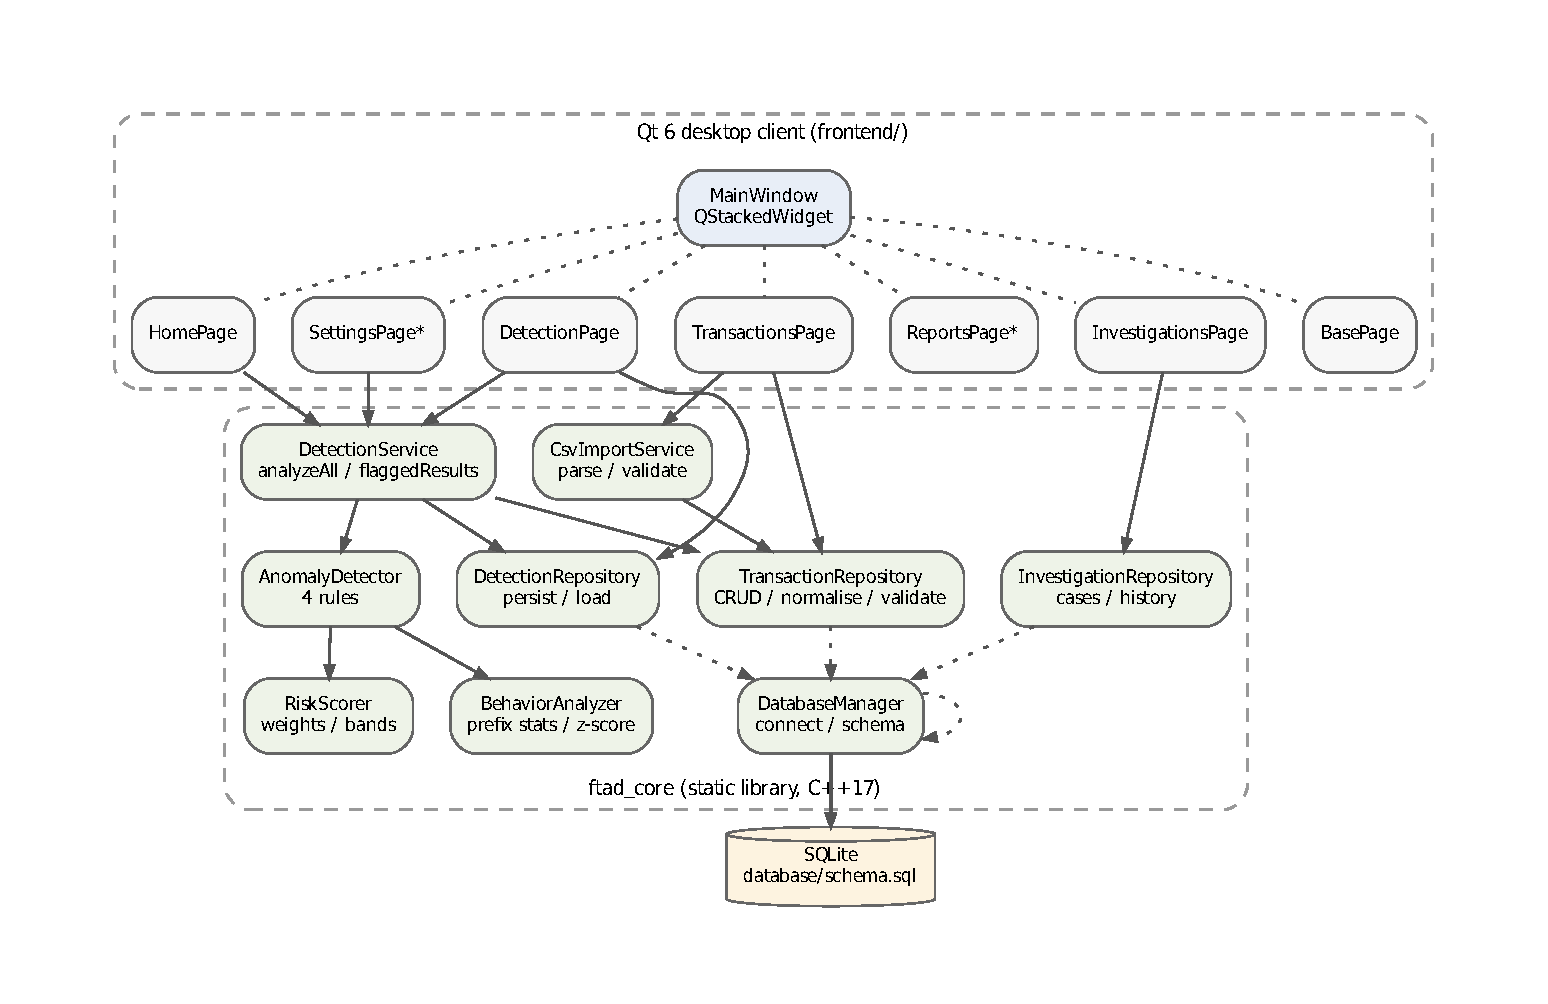
\includegraphics[width=1\textwidth,height=\textheight]{figures/system_architecture.pdf}
\caption{Figure G.1 --- Layering and call relationships. The Qt client
sits above the \texttt{ftad\_core} static library, which is the only
component that touches SQLite. \texttt{ReportsPage} and
\texttt{SettingsPage} (asterisked) are placeholders.}
\end{figure}

\begin{figure}
\centering
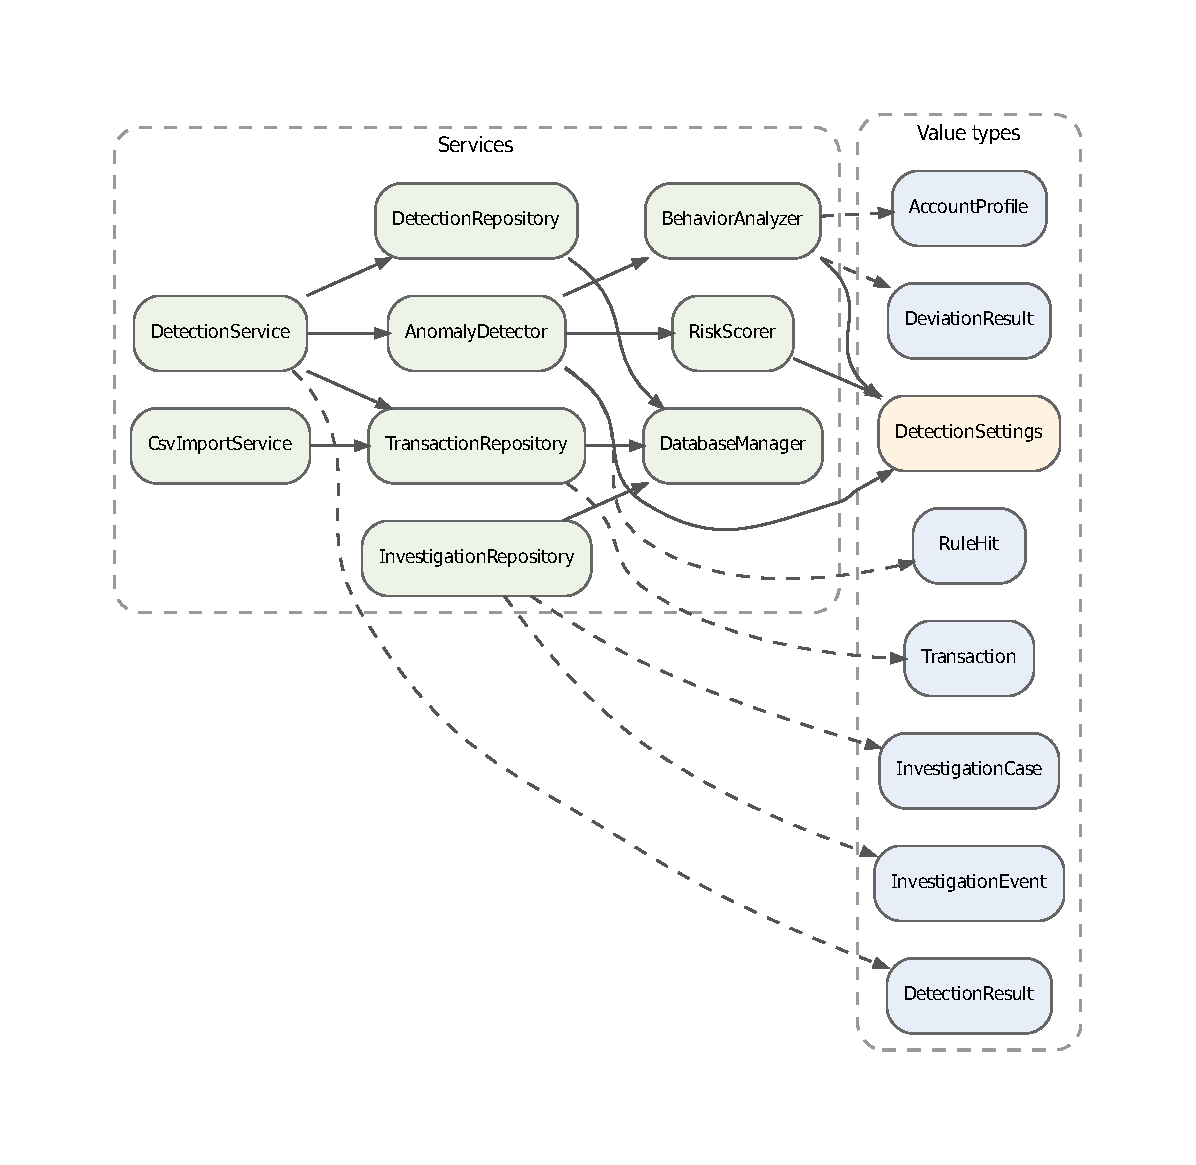
\includegraphics[width=0.95\textwidth,height=\textheight]{figures/class_diagram.pdf}
\caption{Figure G.2 --- Backend classes. Services on the left
collaborate through the value types on the right;
\texttt{Detection\-Settings} (shaded) is the shared configuration object
that every rule reads.}
\end{figure}

\begin{figure}
\centering
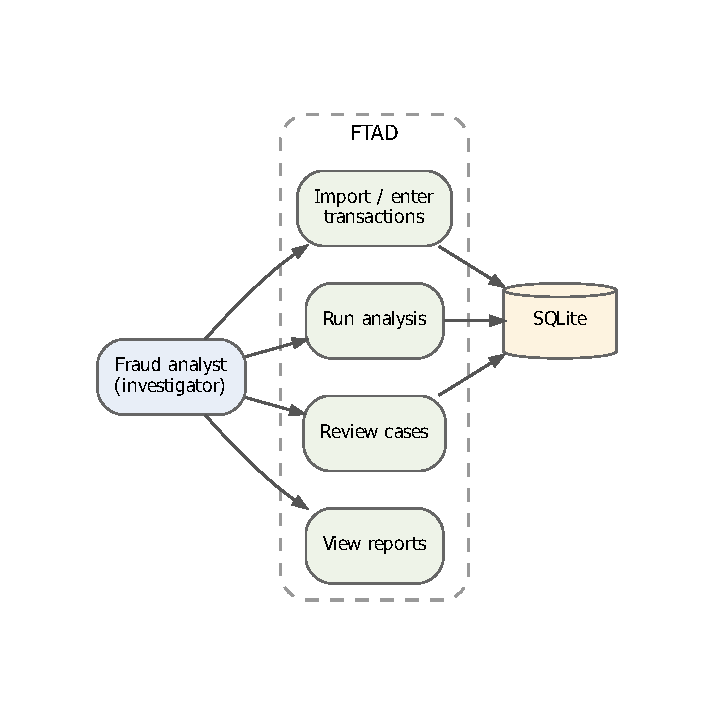
\includegraphics[width=0.62\textwidth,height=\textheight]{figures/use_case.pdf}
\caption{Figure G.3 --- Actors and use cases. A single analyst role
drives import, analysis, case review and reporting, all against the
local database.}
\end{figure}

\begin{figure}
\centering
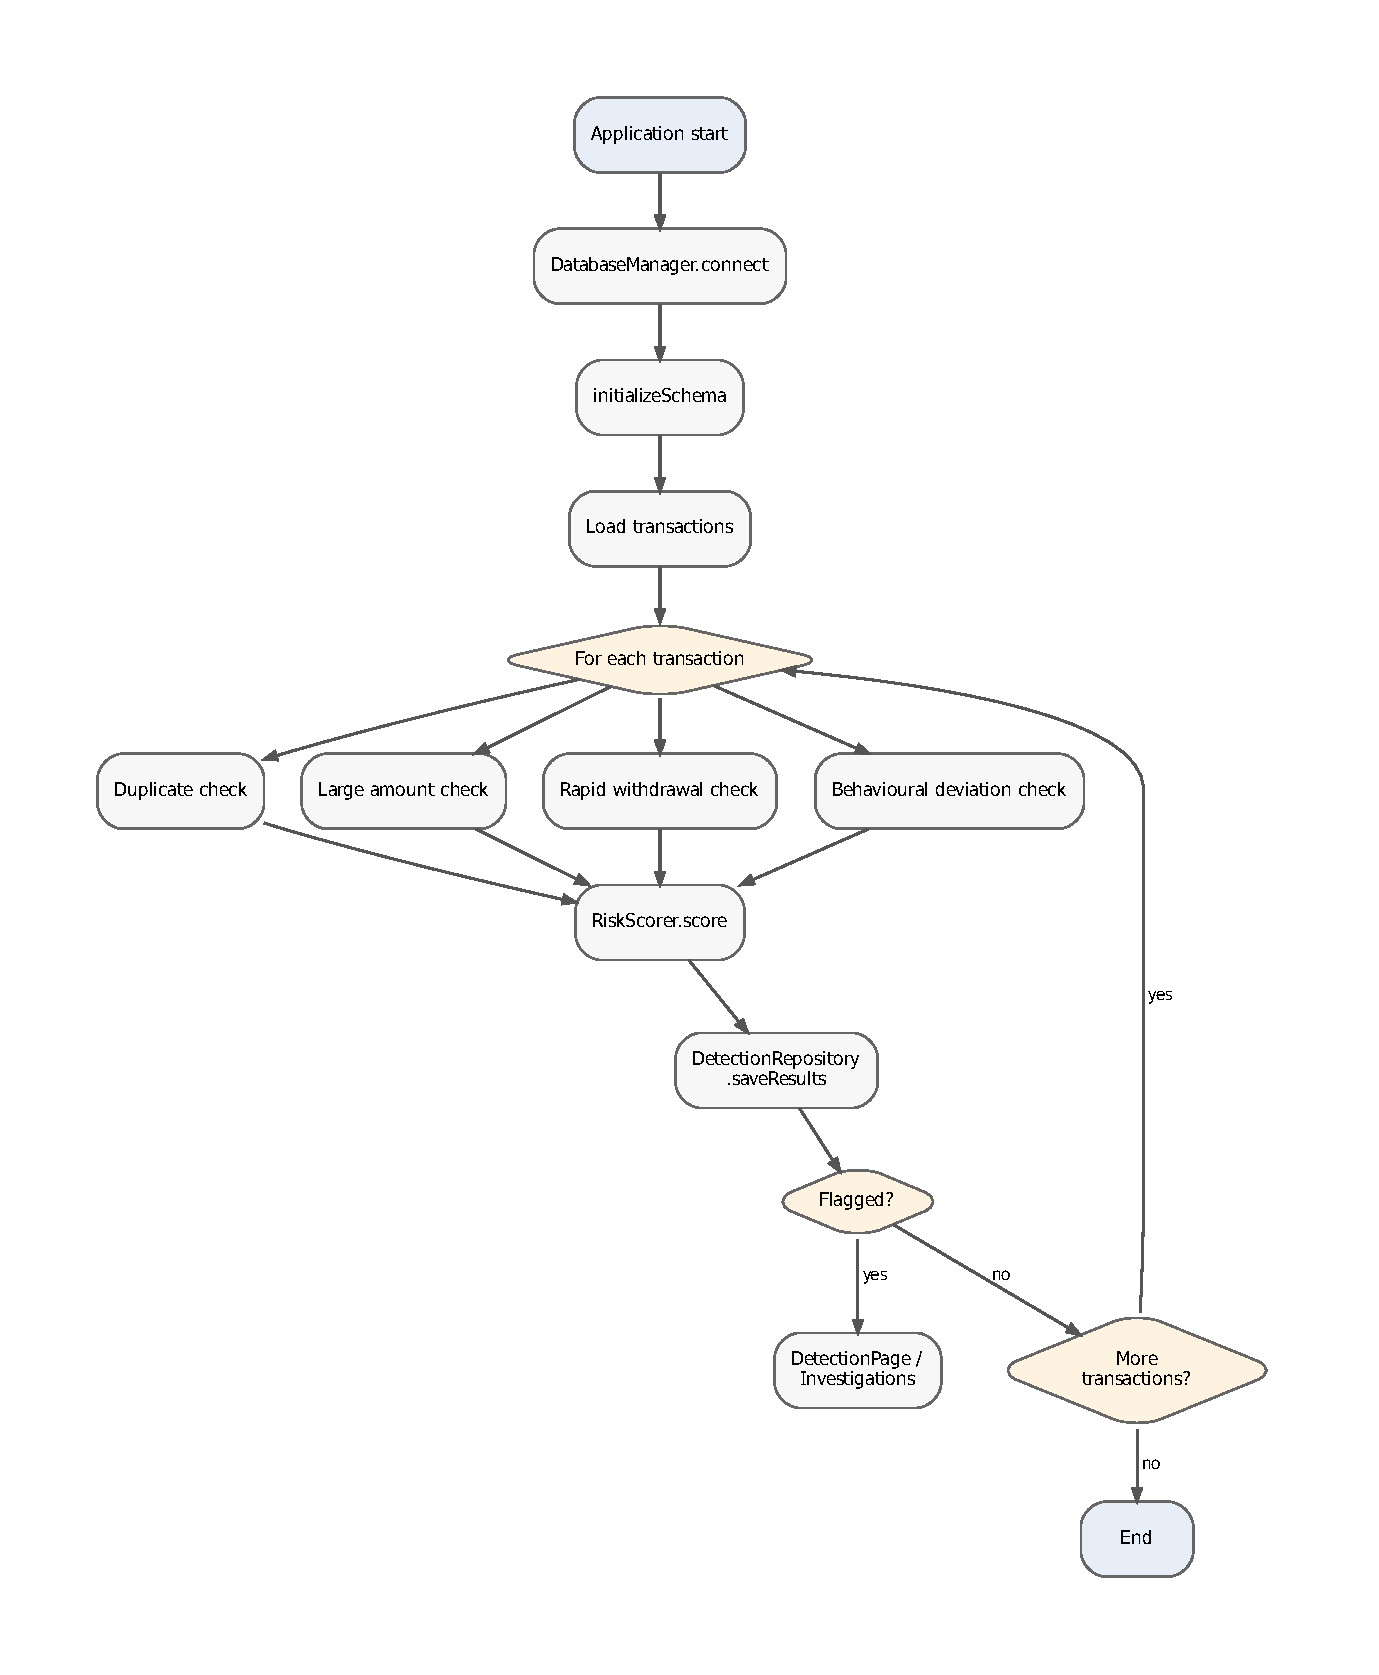
\includegraphics[width=0.88\textwidth,height=\textheight]{figures/activity_detection.pdf}
\caption{Figure G.4 --- Detection activity. Every transaction passes all
four rule checks before scoring, so a single transaction can accumulate
several hits.}
\end{figure}

\begin{figure}
\centering
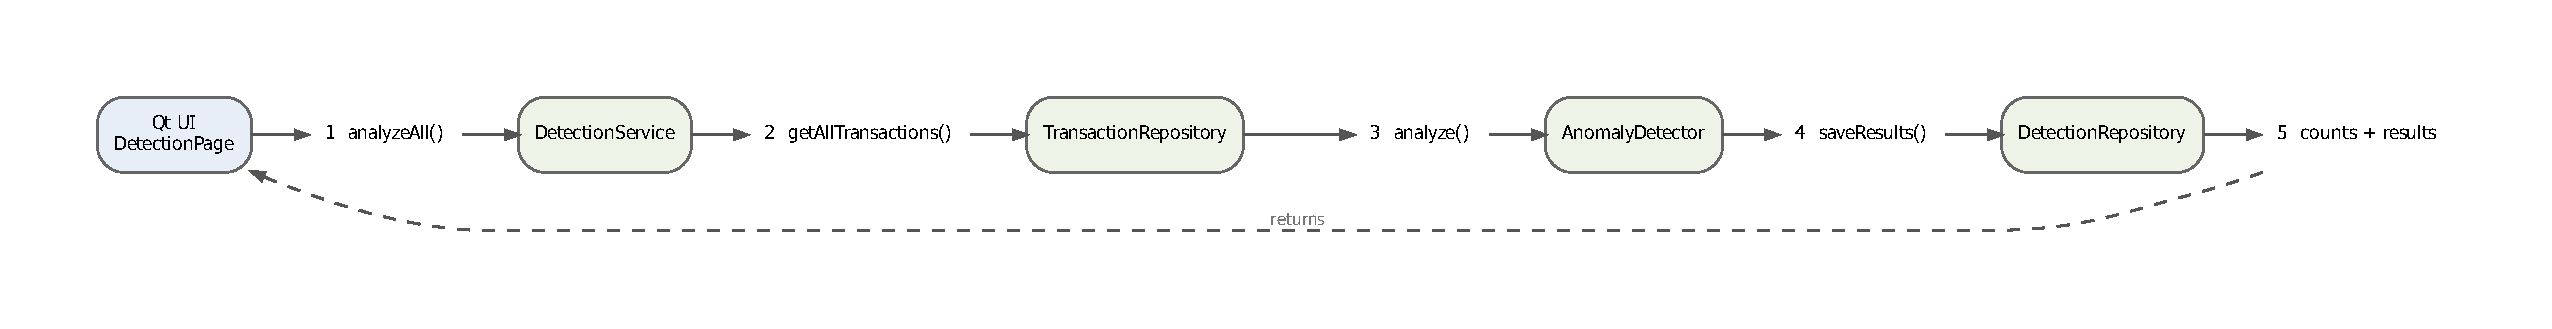
\includegraphics[width=1\textwidth,height=\textheight]{figures/sequence_detection.pdf}
\caption{Figure G.5 --- Call sequence for one analysis pass, from the UI
through \texttt{Detection\-Service} to persistence and back.}
\end{figure}

\begin{figure}
\centering
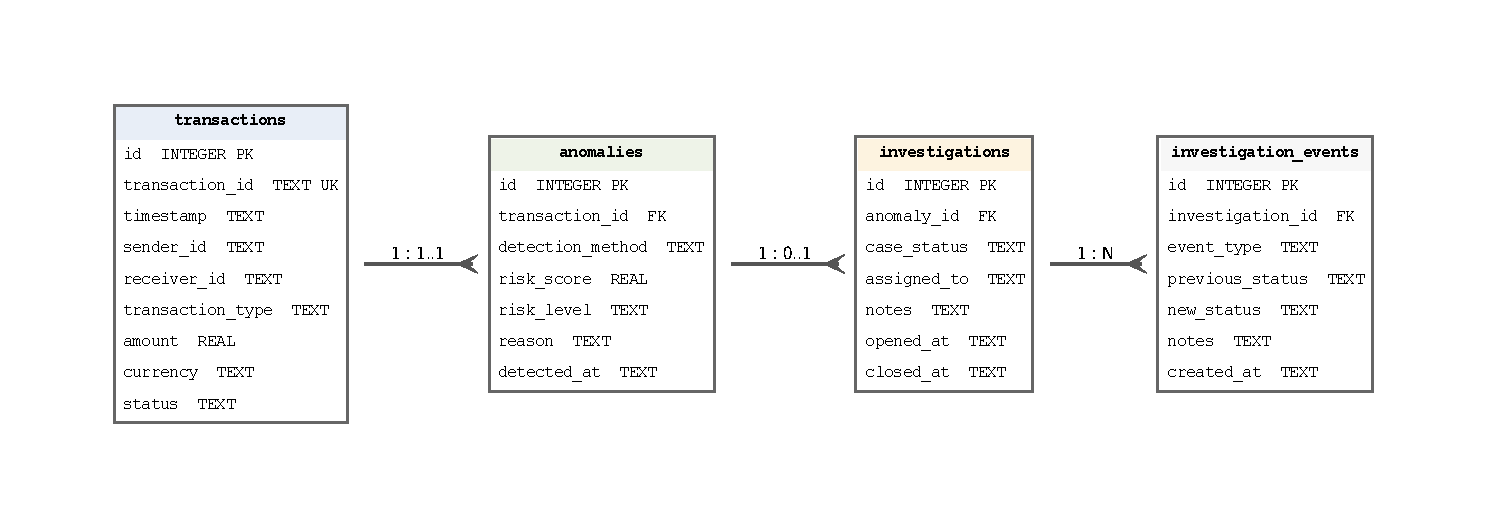
\includegraphics[width=1\textwidth,height=\textheight]{figures/erd.pdf}
\caption{Figure G.6 --- Entity relationships. Foreign keys run
transactions → anomalies → investigations → investigation\_events, with
cascade deletes in the same direction.}
\end{figure}

\end{document}
